%=====================================================================
%  main.tex  –  Master file for the NeurIPS submission
%=====================================================================
\documentclass{article}

% Suppress benign warnings
\usepackage{silence}
\WarningFilter{microtype}{Command \showhyphens has changed}
\WarningFilter{hyperref}{Ignoring empty anchor}

% Recommended, but optional, packages for figures and better typesetting:
\usepackage{microtype}
\usepackage{graphicx}
\usepackage{subcaption}
\usepackage{booktabs} % for professional tables

% hyperref makes hyperlinks in the resulting PDF.
\usepackage{hyperref}

% Attempt to make hyperref and algorithmic work together better:
\newcommand{\theHalgorithm}{\arabic{algorithm}}

% Use the following line for the initial blind version submitted for review:
\usepackage{neurips_2026}

% For preprint, use
% \usepackage[preprint]{neurips_2026}

% If accepted, instead use the following line for the camera-ready submission:
% \usepackage[final]{neurips_2026}

%---------------------------------------------------------------------
% Global package imports
%---------------------------------------------------------------------
% ------------------------------------------------- 
%  Global LaTeX package imports
%  (All packages are loaded once, in a logical order,
%   with no duplicate entries.)
% ------------------------------------------------- 

%--- Core encoding and font handling --------------------------------------------
\usepackage{iftex}
\ifPDFTeX
  % pdfLaTeX (Overleaf default)
  \usepackage[T1]{fontenc}
  \usepackage[utf8]{inputenc}
  \usepackage{times}
\else
  % XeLaTeX (Local Tectonic) or LuaLaTeX
  \usepackage{fontspec}
  \setmainfont{Nimbus Roman}
  \setsansfont{Nimbus Sans}
  \setmonofont{Nimbus Mono PS}
\fi

%--- Mathematics ---------------------------------------------------------------
\usepackage{amsmath,amssymb,amsthm}   % AMS math environments and symbols
\usepackage{mathtools}                % Extensions to amsmath (optional but useful)

%--- Graphics & figures ---------------------------------------------------------
%\usepackage{graphicx}                % (Loaded by ICML template)
\usepackage{tikz}                    % Vector graphics language
\usepackage{pgfplots}                % Plotting with pgf/TikZ
\pgfplotsset{compat=1.17}            % Compatibility version for pgfplots
\usepackage{wrapfig}                 % Text wrapping around figures
%\usepackage{subcaption}              % (Loaded by ICML template)
\usepackage{caption}                 % Caption customisation
\usepackage{float}                   % Improved float placement (e.g., [H])
\usepackage{adjustbox}               % Box-adjustment utilities

%--- Tables --------------------------------------------------------------------
%\usepackage{booktabs}                % (Loaded by ICML template)
\usepackage{tabularx}                % Flexible column widths
\usepackage{multirow}                % Multi-row cells
\usepackage{siunitx}                 % Typeset numbers and units
\sisetup{
    round-mode             = places,
    round-precision        = 3,
    table-alignment-mode   = none,
    % New v3 replacement for all "detect" options:
    mode                   = match,
    reset-text-family      = false,
    reset-text-series      = false
}
%\usepackage{array}                   % Extended column definitions (optional)

%--- Algorithms ---------------------------------------------------------------
%\usepackage{algorithm}               % (Loaded by icml2026.sty)
%\usepackage{algorithmic}             % (Loaded by icml2026.sty)

%--- Hyperlinks & cross-references ---------------------------------------------
%\usepackage{hyperref}                % (Loaded by ICML template)
\usepackage{cleveref}                % Smart cross-reference formatting
\usepackage{url}                     % URL typesetting (fallback for hyperref)
\usepackage{xurl}                     % Allow breaks anywhere in long URLs
\usepackage{doi}                     % DOI hyperlink formatting

%--- Glossaries / Acronyms ------------------------------------------------------
\usepackage[acronym]{glossaries}     % Acronym handling (acronym list)
\makeglossaries                       % Initialise glossaries (called once)

%--- Miscellaneous -------------------------------------------------------------
\usepackage{xcolor}                  % Colour definitions
%\usepackage{microtype}               % (Loaded by ICML template)
\usepackage{enumitem}                % Customisable list environments
\usepackage{float}                   % (already loaded above – kept for clarity)
\usepackage{todonotes}
\usepackage{csvsimple}               %  Csv loading

%--- User-defined helper commands -----------------------------------------------
% Circled characters (used throughout the manuscript)
\newcommand*\circled[1]{
  \tikz[baseline=(char.base)]{
    \node[shape=circle,draw,inner sep=2pt] (char) {#1};
  }
}               % Loads all required \usepackage statements

%---------------------------------------------------------------------
% Global macro definitions
%---------------------------------------------------------------------
% ==============================================================
%  Custom Commands – Global LaTeX configuration
%  --------------------------------------------------------------
%  This file is loaded **after** `latex/packages.tex` (which
%  supplies all required \usepackage statements) and **before**
%  any manuscript section files are \input.
%  It aggregates:
%    • the unmodified ICLR math-macro file (math_commands.tex)
%    • theorem / proof environment definitions
%    • cleveref name customisations
%    • acronym/glossary definitions
%    • project-specific mathematical shortcuts
% ==============================================================

% -------------------------------------------------
% Load the original ICLR math macro file
% -------------------------------------------------
\input{math_commands}

% -------------------------------------------------
% Load theorem/proof environment definitions
% -------------------------------------------------
% --------------------------------------------------------------
%  Theorem/Proof environments
% --------------------------------------------------------------

\usepackage{amsthm}   % Ensure the amsthm package is loaded (already in packages.tex)

\newtheorem{theorem}{Theorem}[section]
\newtheorem{lemma}[theorem]{Lemma}
\newtheorem{corollary}[theorem]{Corollary}
\theoremstyle{definition}
\newtheorem{definition}[theorem]{Definition}
\newtheorem{assumption}[theorem]{Assumption}
\newtheorem{example}[theorem]{Example}
\theoremstyle{remark}
\newtheorem{remark}[theorem]{Remark}

% -------------------------------------------------
% Load cleveref name customisations
% -------------------------------------------------
% -------------------------------------------------
% cleveref name customisations (short forms for cross-references)
% -------------------------------------------------

\crefname{section}{Sec.}{Secs.}
\Crefname{section}{Section}{Sections}
\crefname{figure}{Fig.}{Figs.}
\Crefname{figure}{Figure}{Figures}
\crefname{table}{Tab.}{Tabs.}
\Crefname{table}{Table}{Tables}
\crefname{equation}{Eq.}{Eqs.}
\Crefname{equation}{Equation}{Equations}
\crefname{algorithm}{Alg.}{Algs.}
\Crefname{algorithm}{Algorithm}{Algorithms}

% -----------------------------------------------------------------
% Short-hand macros for appendix references
% -----------------------------------------------------------------
\newcommand{\appsing}{App.}
\newcommand{\applur}{Apps.}


% -------------------------------------------------
% 4. Load acronym definitions (glossaries)
% -------------------------------------------------
\usepackage[acronym]{glossaries}
\makeglossaries

% -----------------------------------------------------------------
% Core acronyms used throughout the manuscript
% -----------------------------------------------------------------
\newacronym{CPM}{CPM}{counts per million}
\newacronym{crl}{CRL}{causal representation learning}
\newacronym{dag}{DAG}{directed acyclic graph}
\newacronym{grbf}{GRBF}{Gaussian Radial Basis Function}
\newacronym{ko}{KO}{knock-out}
\newacronym{pdf}{PDF}{Probability Density Function}
\newacronym{pmf}{PMF}{Probability Mass Function}
\newacronym{cdf}{CDF}{Cumulative Distribution Function}

% -----------------------------------------------------------------
% RAPTORGraph – long form contains bold-face markup
% -----------------------------------------------------------------
\newacronym[
    short = {RAPTORGraph},
    long  = {%
        \textbf{R}esponse%
        \ \textbf{A}nalysis%
        \ of\ \textbf{P}erturbed%
        \ \textbf{T}ranscript\textbf{O}mes%
        \ using\ Inte\textbf{R}pretable\ \textbf{Graph}%
    }
]{raptorgraph}{RaptorGraph}{Response Analysis of Perturbed Transcriptomes using Interpretable Graph}

% -----------------------------------------------------------------
% Additional domain-specific acronyms
% -----------------------------------------------------------------
\newacronym{ot}{OT}{optimal transport}
\newacronym{scATACseq}{scATAC-seq}{single-cell assay for transposase-accessible chromatin using sequencing}
\newacronym{scRNAseq}{scRNA-seq}{single-cell RNA sequencing}
\newacronym{scm}{SCM}{structural causal model}
\newacronym{silu}{SiLU}{Sigmoid Linear Unit}
\newacronym{TPM}{TPM}{transcripts per million}
\newacronym{vae}{VAE}{Variational Autoencoder}
\newacronym{mse}{MSE}{Mean Squared Error}
\newacronym{mmd}{MMD}{Maximum Mean Discrepancy}
\newacronym{rkhs}{RKHS}{Reproducing Kernel Hilbert Space}
\newacronym{dvae}{dVAE}{DiscrepancyVAE}
\newacronym{emd}{EMD}{Earth Mover's Distance}
% -----------------------------------------------------------------
% Miscellaneous textual macro (not an acronym)
% -----------------------------------------------------------------
\newcommand{\insilico}{\emph{in silico}}
\newcommand{\apriori}{\emph{a priori}}
\newcommand{\invitro}{\emph{in vitro}}

% -------------------------------------------------
% Project-specific math shortcuts (vectors, operators, etc.)
% -------------------------------------------------
% --- Vector- and matrix-notation -------------------------------------------------

\newcommand{\vect}[1]{\mathbf{\MakeLowercase{#1}}}
\newcommand{\mat}[1]{\mathbf{\MakeUppercase{#1}}}
\newcommand{\hadamard}[1]{#1 \circ #1}

% -- General Variables & Matrices --
\newcommand{\realnumbers}{\mathbb{R}}
\newcommand{\variables}{\rvx}
\newcommand{\latentvars}{\rvz}
\newcommand{\noiseterms}{\rve}
\newcommand{\adjacencymatrix}{\mB}
\newcommand{\weightmatrix}{\mW}
\newcommand{\identitymatrix}{\mI}
\newcommand{\datamatrix}{\mX}
\newcommand{\interactionmatrix}{\mW_{\text{int}}}

% -- Graph-related --
\newcommand{\graph}{\gG}

% -- SCM / Causal Variables --
\newcommand{\latentcausalvars}{\rvu}
\newcommand{\latentcausalvar}{\ervu}
\newcommand{\exonoise}{\rvz}
\newcommand{\graphmatrix}{\mA}
\newcommand{\structuralfunc}{f}

% -- DAG Operators --
\DeclareMathOperator{\parentnodes}{Pa_{\graph}}
\DeclareMathOperator{\tr}{Tr}
\newcommand{\transitiveclosure}[1]{\bar{#1}}

% -- Dimensionality --
\newcommand{\observeddim}{n}
\newcommand{\latentdim}{d}
\newcommand{\numpathways}{\latentdim}
\newcommand{\numgenes}{\observeddim}
\newcommand{\numperturbedgenes}{k}
% \newcommand{\numparallellayers}{M}
\newcommand{\numgraphs}{m}

% -- Identifiability and Equivalence Classes --
\newcommand{\simT}{\sim_T}
\newcommand{\simC}{\sim_C}

% -- Specific Latent Variables & Model Functions --
\newcommand{\idealencoder}{f^*}
\newcommand{\practicalencoder}{f_\theta}
\newcommand{\latentideal}{\tilde{\rvz}}
\newcommand{\latentchangeideal}{\Delta\tilde{\rvz}}
\newcommand{\causallatentchangeideal}{\Delta\tilde{\rvu}}
\newcommand{\latentchangeapprox}{\Delta\rvz}
\newcommand{\causallatentchangeapprox}{\Delta\rvu}
\newcommand{\maskvector}{\vm}
\newcommand{\interventionstrength}{c}
\newcommand{\conditionvector}{\vc}
\newcommand{\zobs}{\latentvars_{\text{obs}}}
\newcommand{\zint}{\latentvars_{\text{int}}}
\newcommand{\pathwayactivation}{\vect{s}}
\newcommand{\activationfunc}{\rho}
\newcommand{\gumbeltemp}{\tau}

% --- Intervention Encoder Model ---
%\newcommand{\conditionalnet}{g_\phi}
\newcommand{\interventionencoder}{q_{\text{int}}}
%\newcommand{\interventionencoder}{\phi}

% -- Loss Functions and Operators --
\newcommand{\mseloss}{\mathcal{L}_{\text{MSE}}}
\newcommand{\kldloss}{\mathcal{L}_{\text{KL}}}
\newcommand{\mmdloss}{\mathcal{L}_{\text{MMD}}}
\newcommand{\dagmaloss}{\mathcal{L}_{\text{DAGMA}}}
\newcommand{\totalloss}{\mathcal{L}_{\text{total}}}
\newcommand{\acyclicityfunc}{h}
\newcommand{\scorefunc}{S}

% -- Hyperparameters --
% Note: Use standard LaTeX commands \mu and \alpha for these
\newcommand{\scorelambda}{\lambda_{\text{score}}}
\newcommand{\alpharec}{\alpha_{\text{rec}}}
\newcommand{\betakl}{\beta_{\text{KL}}}
\newcommand{\gammammd}{\gamma_{\text{MMD}}}
\newcommand{\deltadagma}{\delta_{\text{DAGMA}}}


% --- MMD Hyperparameters ---
\newcommand{\mmdsigma}{\sigma}
\newcommand{\mmdsigmaMMD}{\sigma_{\text{MMD}}}
\newcommand{\mkmmdweights}{\beta}
\newcommand{\numkernels}{L}
\newcommand{\numsamplesobs}{i} % Changed
\newcommand{\numsamplespred}{j} % Changed


% -- Other Functions and Models --
\newcommand{\truemixingfunc}{g^*}
\newcommand{\decoder}{g}
\newcommand{\normaldist}{\gN}
\newcommand{\betavae}{$\beta$-VAE}


% --- Additional Variables from Synthesis ---
\newcommand{\polydegree}{p}
\newcommand{\learnedrepresentation}{\hat{\latentvars}}
\newcommand{\predictedvariable}{\hat{\variables}}
\newcommand{\predicteddatamatrix}{\hat{\mX}}
\newcommand{\composedfunc}{a}
\newcommand{\affinetransform}{\mat{A}}
\newcommand{\affineoffset}{\vect{c}}
\newcommand{\scalefactor}{e}
\newcommand{\shiftoffset}{b}
\newcommand{\latentsupport}{\mathcal{Z}}
\newcommand{\observsupport}{\mathcal{X}}
\newcommand{\interventionaldist}{P_Z^{(i)}}
\newcommand{\interventionset}{I_k}
\newcommand{\interventiontargets}{\vt_i}
\newcommand{\auxvar}{\vu}

% --- Downstream Analysis Metrics ---
\newcommand{\effectvector}{\Delta}
\newcommand{\ltwonorm}[1]{\left\lVert #1 \right\rVert_2}
\newcommand{\cossim}[2]{\cos\left(#1, #2\right)}
\newcommand{\meanexpression}{\bar{\variables}}
\newcommand{\numcells}{N}
\newcommand{\predictionfunc}{f}
\newcommand{\effectvectornaive}{\effectvector(A+B)_{\text{naive}}}
\newcommand{\synergyscore}{\text{Synergy Ratio}}
\newcommand{\neomorphismscore}{\text{Neomorphism Score}}
\newcommand{\redundancyscore}{\text{Redundancy Score}}
\newcommand{\epistasiscore}{\text{Epistasis Score}}


% --- PROBABILITY OPERATORS (PMF/GENERAL) ---
\newcommand{\prob}[1]{\operatorname{P}\left(#1\right)}
\newcommand{\condprob}[2]{\operatorname{P}\left(#1 \mid #2\right)}

% --- PROBABILITY DENSITY OPERATORS (PDF) ---
\newcommand{\pdf}[1]{\operatorname{p}\left(#1\right)}
\newcommand{\condpdf}[2]{\operatorname{p}\left(#1 \mid #2\right)}

% --- CUMULATIVE DISTRIBUTION OPERATORS (CDF) ---
\newcommand{\cdf}[1]{\operatorname{F}\left(#1\right)}
\newcommand{\condcdf}[2]{\operatorname{F}\left(#1 \mid #2\right)}

% --- STATISTICAL OPERATORS ---
% \DeclareMathOperator{\E}{\mathbb{E}}

% --- DISTRIBUTION METRIC OPERATORS ---
\newcommand{\kernel}{k}
\newcommand{\mmd}{\operatorname{MMD}}
\newcommand{\mkmmd}{\mmd}

% --- CSV LOADING AND STYLING
\newcommand{\makerow}[2]{%
  \pgfplotstableread[col sep=comma]{#1}\loadedtable
  #2 &
  \pgfplotstablegetelem{0}{synergy}\of{\loadedtable}\pgfplotsretval $\pm$ \pgfplotstablegetelem{1}{synergy}\of{\loadedtable}\pgfplotsretval &
  \pgfplotstablegetelem{0}{suppression}\of{\loadedtable}\pgfplotsretval $\pm$ \pgfplotstablegetelem{1}{suppression}\of{\loadedtable}\pgfplotsretval &
  \pgfplotstablegetelem{0}{neomorphism}\of{\loadedtable}\pgfplotsretval $\pm$ \pgfplotstablegetelem{1}{neomorphism}\of{\loadedtable}\pgfplotsretval &
  \pgfplotstablegetelem{0}{redundancy}\of{\loadedtable}\pgfplotsretval $\pm$ \pgfplotstablegetelem{1}{redundancy}\of{\loadedtable}\pgfplotsretval &
  \pgfplotstablegetelem{0}{epistasis}\of{\loadedtable}\pgfplotsretval $\pm$ \pgfplotstablegetelem{1}{epistasis}\of{\loadedtable}\pgfplotsretval \\
}

% --- Revision Highlight Macro ---
% Switch to simple #1 to disable coloring
\newcommand{\revised}[1]{\color{black}{#1}}

% --- Divergence Operators ---
\newcommand{\kl}[2]{\KL(#1 \parallel #2)}

% --- Project Terminology ---
\newcommand{\cmp}{causal meta-pathway}
\newcommand{\cmps}{causal meta-pathways}
        % Loads macros, math shortcuts, etc.

%---------------------------------------------------------------------
% NeurIPS Title and Authors
%---------------------------------------------------------------------
%\title{RAPTORGraph: Graph-Based Pathway Modeling for Causal Discovery in Single-Cell Perturbations}

%\title{Modeling Single-Cell Perturbations through Interpretable Causal Latent Structure with identifiability guarantees}
\title{Learning Interpretable Causal Latent Structure for Genetic Perturbations with Identifiability Guarantees}
%\title{Single-Cell Perturbation Prediction with Interpretable Causal Latent Structure}

%\author{%
%  Anonymous Authors
%}

\begin{document}

\maketitle

% Reset glossary entries so that the first use prints the long form
\glsresetall

\begin{abstract}
Experiments involving perturbation of single cells are central to understanding cellular mechanisms and accelerating therapeutic discovery,  however the space of combinatorial perturbations is intractably large. 
Causal representation learning has shown great promise for predicting unseen combination of perturbations, but existing methods often violate the theoretical requirements for identifiability guarantees.  
We introduce \glsentryshort{raptorgraph}, an end-to-end VAE framework that addresses these issues through: i) a preconditioned \emph{GraphPathway} encoder that enforces soft intervention-guided mappings to \cmps{}, enabling clean single latent-node interventions needed for causal identifiability, and ii) optimal-transport alignment that aligns control and perturbed populations to stabilize conditional generation. 
Empirical results on Perturb-seq datasets demonstrate that \glsentryshort{raptorgraph} improves the trade-off between reconstruction fidelity and distributional matching, and yields improved performance on predicting non-additive combinatorial effects. 
Finally, we show that \glsentryshort{raptorgraph} recovers biologically meaningful latent programs and a causal graph over meta-pathways, providing an interpretable bridge between generative quality and mechanistic insight.
\end{abstract}
% \begin{abstract}
%
% Experiments involving the perturbation of individual cells are central to understanding cellular mechanisms and can accelerate drug discovery.
% \Gls{crl} allows us to uncover the latent factors that regulate biological systems and predict the impact of novel perturbations.
% Unfortunately, existing methods fail to address intervention spillover in a closed-world setting where intervention targets are known \apriori, such as in Perturb-seq experiments, due to their reliance on dense encoders.
% Furthermore, incorporating curated biological pathways into the model imposes a confirmatory bias, forcing it to explain the data through preexisting pathways and reducing the set of hypotheses the model can explore, while discarding novel signals that lie outside the annotated pathways.
% In this work, we introduce \glsentryshort{raptorgraph}, a \betavae{} with a GraphPathway encoder that explicitly models complex gene-to-gene interactions within learned pathways.
% Moreover, our model's preconditioning isolates the influence of perturbed genes, yielding clean, single-node latent interventions required for identifiable causal discovery and eliminating spillover.
% Finally, we train the model on data preprocessed with optimal-transport alignment, which guarantees a well-defined mapping between control and perturbed samples and further stabilizes the learned latent representations.
% We demonstrate that \glsentryshort{raptorgraph} improves state-of-the-art performance on downstream analyses of unseen perturbations, such as non-additive interactions, while outperforming other approaches on objective metrics, such as \glsentryshort{mse} and \glsentryshort{mkmmd}.
% The code will be made publicly available upon publication of this paper.
%
% \end{abstract}


% Original Abstract (Reference)
% \begin{abstract}
%
% Experiments involving the perturbation of individual cells are central to understanding cellular mechanisms and can accelerate drug discovery.
% \Gls{crl} allows us to uncover the latent factors that regulate biological systems and predict the impact of novel perturbations.
% Unfortunately, existing methods fail to address intervention spillover in a closed-world setting where intervention targets are known \apriori, such as in Perturb-seq experiments, due to their reliance on dense encoders.
% Furthermore, incorporating curated biological pathways into the model imposes a confirmatory bias, forcing it to explain the data through preexisting pathways and reducing the set of hypotheses the model can explore, while discarding novel signals that lie outside the annotated pathways.
% In this work, we introduce \glsentryshort{raptorgraph}, a \betavae{} with a GraphPathway encoder that explicitly models complex gene-to-gene interactions within learned pathways.
% Moreover, our model's preconditioning isolates the influence of perturbed genes, yielding clean, single-node latent interventions required for identifiable causal discovery and eliminating spillover.
% Finally, we train the model on data preprocessed with optimal-transport alignment, which guarantees a well-defined mapping between control and perturbed samples and further stabilizes the learned latent representations.
% We demonstrate that \glsentryshort{raptorgraph} improves state-of-the-art performance on downstream analyses of unseen perturbations, such as non-additive interactions, while outperforming other approaches on objective metrics, such as \glsentryshort{mse} and \glsentryshort{mmd}.
% The code will be made publicly available upon publication of this paper.
%
% \end{abstract}

\glsresetall

%---------------------------------------------------------------------
% Content Injection
%---------------------------------------------------------------------
%===============================================================================
\section{Introduction}
\label{sec:introduction}
%===============================================================================

Understanding how cells respond to genetic perturbations, such as those induced by CRISPR screens~\citep{dixit2016perturb}, is fundamental to understand disease biology and advancing therapeutic discovery ~\citep{plenge2013validating,adamson2016multiplexed,norman2019exploring}. 
However, the combinatorial explosion across $\sim$25,000 genes makes exhaustive perturbation experiments infeasible~\citep{norman2019exploring}, motivating computational models that predict cellular responses to unseen perturbations or combinations thereof.

Existing approaches to predict the transcriptional outcome following a perturbation face a fundamental challenge: generative quality comes at the cost of causal interpretability.
For example, recent methods like GEARS~\citep{roohani2024predicting} or scGPT~\citep{cui2024scgpt} achieve strong predictive performance in cellular response to perturbations; however, they act as ``black boxes'' providing little mechanistic insight into how perturbations affect cellular systems,
%This opacity prevents researchers from understanding why certain combinations of perturbations produce synergistic effects, 
failing to provide testable biological hypotheses.


Computational biology demands models that provide mechanistic insights into cellular function~\citep{chen_applying_2024}, making \gls{crl}~\citep{scholkopf2021toward} a promising approach for mapping (intervened) genes to biological processes.
Recent \gls{crl} approaches such as \gls{dvae}~\citep{zhang2023identifiability} or SENA~\citep{de2025interpretable} aim at recovering the underlying causal factors aligned with the interventions, enabling counterfactual reasoning.
However, these \gls{crl} approaches suffer from a fundamental architectural limitation: a dense interventional encoder allows every gene, including the intervened ones, to influence many or all latent variables, undermining the requirements for their identifiability guarantees.
We term this phenomenon \emph{intervention spillover}, which renders identifying the unique latent target for a given intervention ill-posed.
Consequently, the intervention mechanism cannot perform the clean, single-node manipulation required for valid causal inference~\citep{brehmer2022weakly,lippe2022citris}.

\revised{Further, the destructive nature of \gls{scRNAseq} makes it impossible to observe the same cell before and after a genetic intervention, complicating the prediction of cell-specific responses.
Existing methods address this issue by randomly pairing control and perturbed cells.
Since current models are trained to minimize the error across all possible arbitrary pairings, they are incentivized to (suboptimally) learn the population-mean response.
We refer to this phenomenon as \emph{mean collapse}, as this regression to the mean erodes cellular diversity.}

To address these critical issues, we present \gls{raptorgraph}, a novel framework that addresses causal identifiability challenges through a structured encoder design. 
We first propose a novel GraphPathway layer, which uses preconditioning to enforce sparse mappings from genes to learned interpretable causal factors. We term these factors \emph{\cmps{}}, which encompass the (related) known biological processes associated with a given perturbation.
Our design enables clean, single-node latent associations required for causal inference while  maintaining interpretability.
This innovation is complemented by an \gls{ot} preprocessing step, which mitigates the distinct problem of mean collapse.

\revised{We benchmark \glsentryshort{raptorgraph} on two well-known datasets: the \citet{norman2019exploring} Perturb-seq dataset, and the \citet{replogle_combinatorial_2020} CRISPRi dataset, assessing, among others, the accuracy of inferred genetic interactions under combinations of perturbations, and the biological plausibility of the inferred \cmps{}. We uncover biologically accurate programs, such as differentiation-induced cell cycle arrest driven by EGR1 and the stress-induced growth arrest mediated by JUN.}
%\revised{Additionally, we \citet{replogle_combinatorial_2020} CRISPRi dataset}

%We demonstrate strong performance alongside interpretability, which addresses key gaps not filled by current approaches.

% FILE: sections/02_background.tex

%===============================================================================
% SECTION: BACKGROUND
%===============================================================================
\section{Background}
\label{sec:background}
%===============================================================================

% In this section, we introduce the foundation for \gls{crl}~\citep{scholkopf2021toward} and discuss its application to biological data, where latent variables in a \gls{scm} can represent pathway activities~\citep{de2025interpretable}.
% We also highlight the fundamental issues in current approaches that our framework aims to address.
% For clarity and reference, a full table of notation is included in \cref{app:nomenclature}.

\subsection{Predicting transcriptional responses to unseen genetic perturbations}
%Accurate \insilico{} prediction of perturbation effects remains critical to guide experimental perturbations assays, as they would allow us to predict, for instance, how cells respond to environmental stress~\citep{frangieh2021multimodal}.
%However, 
A key limitation in learning transcriptional  responses to unseen genetic perturbations lies in the destructive nature of scRNA-seq, which prevents measuring the same cell before and after a perturbation. While paired measurements are infeasible, we do have access to independent single-cell observations from control and perturbed cells.

Recent works have demonstrated the potential of representation learning in leveraging perturbation data to predict transcriptional outcomes of novel combinations of perturbations. For example, \citet{kamimoto2023dissecting} relied on inferring (linear) transcriptional relationships between genes in the form of a gene regulatory network to infer the effect of unseen perturbations. The Compositional Perturbation Autoencoder (CPA)~\citep{lotfollahi2023predicting} predicted combinations of perturbations by vector arithmetic in the latent space generated by a \gls{vae}.
In parallel, GEARS~\citep{roohani2024predicting} leveraged Graph Neural Networks (GNNs) to incorporate prior knowledge of gene-gene relationships into the model architecture, thereby predicting unseen genetic interventions and their combinations. CellOT~\citep{bunne2023learning} proposed to directly learn optimal transport maps between control and perturbed cell states, thus accounting for heterogeneous subpopulation structures in the data.
% [ADDITION: Addressing Reviewer 1eZy] Added context for single-cell foundation models (scGPT, Geneformer) 
% to contrast RAPTORGraph's explicit causal focus with statistical correlational embeddings.
Recently, large-scale single-cell foundation models, such as scGPT~\citep{cui2024scgpt} and Geneformer~\citep{theodoris2023transfer}, have explored Transformer-based architectures to learn universal transcriptomic representations. While these models provide powerful embeddings for statistical downstream tasks, they typically capture correlational patterns rather than explicit causal mechanisms. Consequently, they often fail to outperform simpler baselines in predicting complex interventional consequences, such as non-additive interactions.
The non-causal ``black box'' nature of these approaches hampers their capability for uncovering the causal mechanisms driving transcriptional changes.
%
%Even though all the outlined approaches tackle the common problem of predicting the transcriptional consequences of  perturbations, 
%their non-causal ``black box'' nature hampers their capability for uncovering the causal mechanisms driving observed transcriptional changes.
This poses a significant limitation in, for example, cellular engineering, where understanding the \emph{why} behind perturbation effects is as critical as predicting the \emph{what}.


To address this challenge, \gls{dvae}~\citep{zhang2023identifiability} learns causal factors without an explicit semantic meaning, resulting in causally valid but biologically uninterpretable latent representations.
SENA~\citep{de2025interpretable}, on the other hand, explicitly models (a set of) biological processes as \cmps{}, promising both predictive accuracy and mechanistic interpretability. 
%Specifically, SENA learns structured latent spaces where each dimension corresponds to a (set of) biological pathway, and causal relationships between them are explicitly represented through learned graph structures.
%
Further, 
%these methods span a spectrum between fully exploratory and strongly confirmatory causal discovery approaches.
exploratory causal approaches~\citep{pmlr-v235-herrmann24b}, such as \gls{dvae}, learn all latent components directly from data, while more confirmatory models, such as SENA, impose (strong) biological priors to improve interpretability. Although the latter strategy grounds the model in established biology, it can suffer from poor knowledge transfer: biological pathways are highly cell-type- and cell-line-specific~\citep{schneider2017tissue,gamazon2018using,%walter2019biological,
hekselman2020mechanisms}, so mechanisms characterized in one cellular context may not generalize to another.

%-------------------------------------------------------------------------------
% Subsection: Structural Causal Models for Latent Discovery
%-------------------------------------------------------------------------------
\subsection{Modeling biological processes as latent causal variables}
\label{subsec:background:scm}
%-------------------------------------------------------------------------------

We model the underlying data-generating process using a \gls{scm}~\citep{pearl2009causality}.
We assume that observed high-dimensional samples $\variables \in \realnumbers^\observeddim$ (gene expression) are generated by a set of unobserved, low-dimensional \emph{\cmps{}} $\latentcausalvars \in \realnumbers^\latentdim$, where $\latentdim \ll \observeddim$.
Note that these \cmps{} may include several (related) known biological processes or pathways. The \gls{scm} defines the relationships between these variables via a set of structural assignments:
\begin{equation}
    \latentcausalvar_i = \structuralfunc_i(\parentnodes(\latentcausalvar_i), \exonoise_i), \quad \text{for } i=1, \dots, \latentdim
    \label{eq:scm_general}
\end{equation}
where $\structuralfunc_i$ is the structural function, $\parentnodes(\cdot)$ are the direct causal parents under graph $\graph$, and $\exonoise_i$ is an independent exogenous variable.
The complete set of these equations induces a \gls{dag} $\graph$, which implies that the joint probability distribution over $\latentcausalvars$ factorizes as:
\begin{equation}
    \pdf{\latentcausalvars} = \prod_{i=1}^{\latentdim} \pdf{\latentcausalvar_i \mid \parentnodes(\latentcausalvar_i)}
    \label{eq:joint_distribution_factorization}
\end{equation}
However, these \cmps{} are not directly accessible.
Instead, we only observe the high-dimensional data $\variables$, which are generated via a true, unknown mixing function: $\variables = \truemixingfunc(\latentcausalvars)$.

%-------------------------------------------------------------------------------
% Subsection: Identifiability from Targeted Interventions
%-------------------------------------------------------------------------------
\subsection{Identifiability of biological causal factors under genetic interventions}
\label{subsec:background:targeted_interventions}
%-------------------------------------------------------------------------------
%
\begin{wrapfigure}[19]{r}{0.43\textwidth}
\vspace{-5pt}
    \centering
    \vspace{-0.75\baselineskip}
    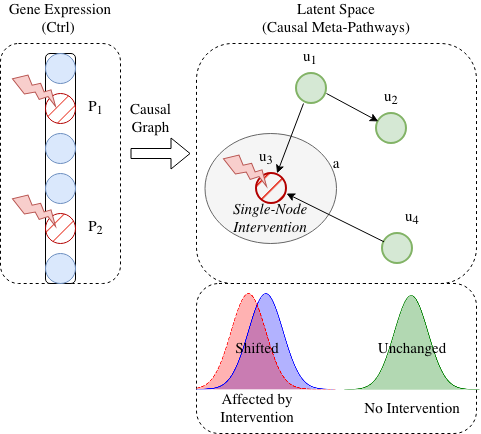
\includegraphics[width=0.98\linewidth]{gfx/Latent_interventions_modified.png}
    \caption{An intervention in gene expression $\variables$ shifts the conditional distribution $p^I(\latentcausalvar_i \mid \parentnodes(\latentcausalvar_i))$ of a single meta-pathway $\latentcausalvar_i$ (causal latent factor), while leaving unrelated latent factors unaffected.}\label{fig:single_node_intervention}
    \vspace{-\baselineskip}
\end{wrapfigure}
%
The central challenge of \gls{crl} is \emph{identifiability}: learning an encoder function $\practicalencoder$ that can uniquely recover the true causal latents $\latentcausalvars$ from the observations $\variables$.
However, when solely using observational data, this goal is theoretically intractable as multiple distinct causal structures
can generate identical observational distributions $\pdf{\variables}$~\citep{pearl2009causality, khemakhem2020variational}.
%
%Additionally, when using \gls{vae}s as the underlying architecture, \citet{khemakhem2020variational} showed that different parameter configurations can generate equivalent marginal distributions $\pdf{\variables}$, leaving the \gls{vae}-learned latent representations non-unique.
%
%In the causal setting, this problem is compounded, as multiple distinct causal structures can generate identical observational distributions.
%This means that learning interpretable causal mechanisms from observational data alone is ill-posed.
%
To overcome this, modern \gls{crl} relies on interventional data, as interventions create unique statistical signatures that break the symmetries present in observational data (Fig. \ref{fig:single_node_intervention}). Thus, identifiability depends on a set of key requirements (\citet{scholkopf2021toward}):

\textbf{Requirement 1 (Acyclic Causal Structure).}
The causal structure is assumed to form a \gls{dag}, a foundational principle in causal discovery~\citep{pearl2009causality}.

\textbf{Requirement 2 (Atomic Interventions).}
%Identifiability theory demonstrates that 
Causal structure recovery % (i.e., identifiability guarantee)
requires access to interventional data that targets each individual latent variable at least once. Atomic interventions are a key assumption in modern \gls{crl}~\citep{zhang2023identifiability, von2023nonparametric, de2025interpretable}.

% \begin{figure}[h]
%     \centering
%     \begin{minipage}{0.52\textwidth}
%         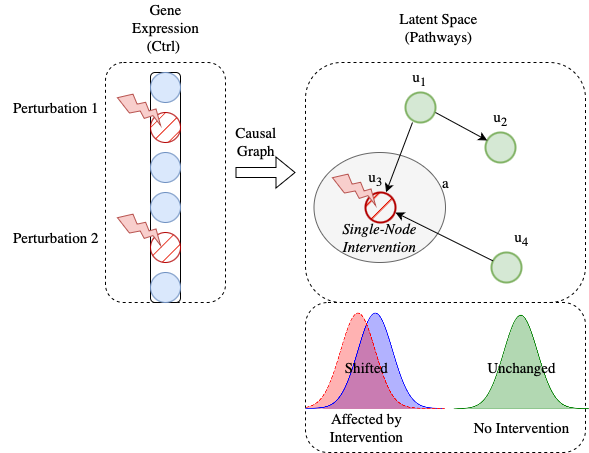
\includegraphics[width=\linewidth]{gfx/Latent_interventions.png}
%     \end{minipage}
%     \hfill
%     \begin{minipage}{0.40\textwidth}
%         \small
%         An intervention in the observed gene expression space $\variables$ causes a shift in a single latent pathway activity $\latentcausalvar_i$.
%         This alters the conditional distribution $p^I(\latentcausalvar_i \mid \parentnodes(\latentcausalvar_i))$ while leaving unrelated latent variables unaffected, a key requirement for identifiability.
%     \end{minipage}
%     \caption{Illustration of an atomic intervention in the latent space.}
%     \label{fig:single_node_intervention}
% \end{figure}

\textbf{Requirement 3 (Faithfulness).}
\gls{crl} also relies on the \emph{faithfulness assumption}, which posits that all conditional independencies in the data are a consequence of the causal graph structure (d-separation) and not due to coincidental cancellations of parameters \cite{zhang2023identifiability} %formalizes two key aspects of this requirement for their setting.
%First, \emph{linear interventional faithfulness} ensures that the effect of an intervention on a descendant is not perfectly cancelled by a linear combination of other variables.
%Second, they assume no perfect cancellation between a direct causal effect and other parallel paths in the graph.

Under these requirements, it is possible to provably recover the true latent causal graph up to a well-defined equivalence class.
Following the work of \citet{zhang2023identifiability}, their main theorem provides a formal guarantee for identifiability:

\begin{theorem}[Full DAG Identifiability, \citet{zhang2023identifiability}]
\label{thm:zhang_full_dag}
Assume a \gls{scm} with a latent \gls{dag} $\graph$ and an invertible mixing function.
If the set of interventions is atomic (targeting each latent variable at least once), and the assumptions of faithfulness hold, then the latent \gls{dag} $\graph$ and the intervention assignments are identifiable up to permutation, scaling, and translation (the CD-equivalence class).
\end{theorem}

The reliance on a \textbf{set of atomic interventions}, where each intervention targets a unique latent factor at least once, is the cornerstone of modern \gls{crl}-based prediction of genetic perturbations \citep{zhang2023identifiability,de2025interpretable}.

%-------------------------------------------------------------------------------
% Subsection: Soft Interventions in Biological Systems
%-------------------------------------------------------------------------------
% \subsection{Soft Interventions in Biological Systems}
% \label{subsec:background:soft_interventions}
% %-------------------------------------------------------------------------------

% An intervention is considered "hard" if it replaces the causal mechanism of a variable entirely (e.g., setting it to a constant), whereas a "soft" intervention only alters the functional relationship to its parent nodes.
% The latter case is particularly relevant for biological data from modern experimental techniques like Perturb-seq~\citep{norman2019exploring}.
% In these \emph{closed-world experiments}, the genetic target of each intervention is known \emph{a priori}, providing a clear causal anchor.

% The study by \citet{norman2019exploring} is a prime example of a soft, gain-of-function intervention.
% It employed a CRISPR activation (CRISPRa) system, which uses a deactivated Cas9 (dCas9) that cannot cut DNA.
% Instead, it recruits transcriptional activators to gene promoters, leading to graded, tunable increases in endogenous gene expression.
% Because this approach modulates gene function rather than ablating it completely, it aligns perfectly with the mathematical definition of a soft intervention.

%-------------------------------------------------------------------------------
% Subsection: The Intervention Spillover Problem
%-------------------------------------------------------------------------------
\subsection{Intervention spillover in dense encoders: challenges for identifiability}
\label{subsec:background:spillover}
%-------------------------------------------------------------------------------

While identifiability theory provides a strong theoretical foundation, a key challenge arises in recent \gls{crl} architectural choices: the \emph{intervention spillover problem}. This phenomenon occur when a single-variable intervention in the high-dimensional observation space $\variables$ is transformed into a multi-variable distributional shift in the lower-dimensional latent space $\latentcausalvars$, which is in  direct conflict with the atomic intervention requirement  (Requirement 2 in \cref{subsec:background:targeted_interventions}). This phenomenon is particularly concerning in genetic perturbation experiments, as interventions are applied to individual genes in the high-dimensional expression space, yet their effects propagate through the cell's regulatory network and manifest as coordinated changes across multiple biological processes. 

\textbf{It is thus crucial to ensure that, for each intervened gene, the sole (causal) latent factor associated with the intervention encompasses all relevant biological processes}. 
%For a more detailed theoretical analysis of this problem, see \cref{app:proofs:spillover}. 
%
%This issue stems from a d
% An \emph{Ideal Causal Encoder}, $\idealencoder$, would satisfy the atomic intervention requirement by ensuring that a single-gene intervention only alters the parameters for the distribution of a single causal latent variable $\causallatentchangeapprox = \idealencoder(\variables_{\text{int}}) - \idealencoder(\variables_{\text{obs}})$.
% Consequently, the expected change in the latent variables would be perfectly sparse, modelled, for example, as $\causallatentchangeideal = \maskvector \cdot \interventionstrength$, where $\maskvector$ is a one-hot vector identifying the single latent target and $\interventionstrength$ is the scalar strength of the intervention (see \cref{fig:single_node_intervention}).
As such, an \emph{Ideal Causal Encoder}, $\idealencoder$, must satisfy atomic intervention by ensuring that an intervention on a single gene generates a distributional effect on a sole latent factor, %yielding a perfectly sparse, manifesting a clean, single-variable intervention  
rather than a dense multi-variable distributional shift.
%
However, interventional encoders $\practicalencoder$ with dense architectures, like MLPs, possess a dense Jacobian matrix, which %meaning that % each component of the latent vector is a function of all input components.
%a sparse change in the input $\variables$ propagates through the network, and  
results in a dense output implicating multiple plausible latent targets. The model is thus forced to select a single ``best'' latent factor whose distribution to shift. This behavior has several critical implications for the reliability of the learned intervention targets (\cref{app:proofs:spillover} for the formal assumptions and the proof of incompatibility of dense architectures). Our proposed architecture, on the other hand, satisfies identifiability while still modeling complex gene-gene relations, by enforcing the mapping to a unique causal latent via preconditioning and a learned DAG. 
%For a mathematical formulation of this ideal behavior, , %and  we refer the reader to %\cref{app:proofs:spillover:setup}, \cref{app:proofs:spillover:assumptions}, and \cref{app:proofs:spillover:lemma_proof}.


%This forces the model to select the  to shift, even when the dense encoder output implicates multiple plausible targets.This means that the model is forced to choose the `best' single (latent) target whose distribution to shift from a dense output that suggests multiple viable targets. 
% Thus the resulting approximated latent change---defined as $\latentchangeapprox = \practicalencoder(\variables_{\text{int}}) - \practicalencoder(\variables_{\text{obs}})$---becomes non-optimal.
%
% This creates a fundamental incompatibility.
% Formally, the model must learn an intervention effect that reconstructs this observed latent change, typically by implicitly minimizing a loss function:
% \begin{equation}
%     \mathcal{L} = || \latentchangeapprox - (\maskvector \cdot \interventionstrength) ||^2
%     \label{eq:spillover_loss}
% \end{equation}
%
 
%First, models that use a softmax function for latent target identification must force a ``winner-take-all'' decision on a dense signal, potentially misattributing the primary causal effect.
%Further, while the perturbed gene is known \emph{a priori}, its associated latent factor is not, making the task of reliably discovering it from an entangled signal intractable.
%This reframes the primary modeling objective: the model should be designed not to explore for a latent target, but to accurately learn the magnitude of the intervention's effect on the causal representation.
%We provide an in-depth discussion about this problem in \cref{app:proofs:spillover}.
%
%In a variational context, the encoder parameterizes the posterior distribution over a set of learned (exogenous) latent variables, from which we sample $\latentvars$. The learned causal graph (the \gls{scm}) then operates on $\latentvars$ to model the causal relationships between the \cmps{} $\latentcausalvars$ (see \cref{eq:scm_general}).
%
%\revised{\textbf{Spillover problem in genetic perturbation prediction}. 
%\textbf{Intervention spillover in current models for genetic perturbation prediction.} 
%

%
%thus crucial to distinguish this intervention spillover, an artifact of dense encoders, from true biological correlation. High correlations between genes do not violate the single-node intervention requirement.
%Rather, dense encoders fail by transforming a sparse perturbation into a dense entry point in the latent space.

%-------------------------------------------------------------------------------
% Subsection: The Role of Prior Knowledge in Causal Modeling
%-------------------------------------------------------------------------------
%\subsection{The Dilemma of Prior Knowledge in Causal Discovery}
%\label{subsec:background:spectrum}
%-------------------------------------------------------------------------------

%\textbf{The dilemma of prior knowledge in causal discovery.} 

%===============================================================================
% SECTION: METHODS
%===============================================================================
\section{RAPTORGraph: model architecture and learning}
\label{sec:methods}
%===============================================================================

\gls{raptorgraph} is an end-to-end framework designed to learn causal relationships from interventional single-cell data (Perturb-seq data). It consists of two novel modules: a preconditioned GraphPathway Encoder~(\cref{subsec:methods:graphpathway}) that maps genes to learned interpretable causal latent factors (the \cmps{})  and a DAGMA-based DAG module~(\cref{subsec:methods:dagma}) that infers the causal graph between the learnt \cmps{}.
The proposed design directly addresses the Intervention Spillover Problem ensuring by construction, ensuring that gene interventions target a unique \cmp{}.
We refer to \cref{app:architecture:overview} for a  detailed description  of the model.

%-------------------------------------------------------------------------------
% Subsection: GraphPathway Encoder for Deconfounding through Preconditioning
%-------------------------------------------------------------------------------
\subsection{GraphPathway encoder with preconditioning}
\label{subsec:methods:graphpathway}
%-------------------------------------------------------------------------------

To address the Intervention Spillover Problem and enforce the theoretical requirement for single-causal-factor interventions, we introduce a novel encoder architecture, the GraphPathway Encoder, which features a deconfounding approach through preconditioning.
This approach requires a specific ordering of the input data.
Let $\numperturbedgenes$ be the number of known perturbed genes in the experiment.
Without loss of generality, we assume the input gene vector $\variables \in \realnumbers^\observeddim$ is sorted such that the first $\numperturbedgenes$ genes are those perturbed, followed by the remaining $\observeddim-\numperturbedgenes$ unperturbed genes.

\textbf{Pre-conditioning module (\cref{fig:arch:graphpathway_encoder}-A)}. Given this sorted input, we define our model with $\latentdim$ learned \cmps{}, where we require that the number of learned \cmps{} is at least the number of perturbed genes ($\latentdim \ge \numperturbedgenes$).
We then structure the encoder's primary weight matrix $\weightmatrix$ as a block matrix that enforces a sparse, one-to-one mapping for perturbed genes while allowing dense interactions for the unperturbed components (see \cref{app:graphpathway} for the formal definition of $\weightmatrix$).

This diagonal structure ensures each of the $\numperturbedgenes$ perturbed genes directly influences only one of the first $\numperturbedgenes$ learned \cmps{} (\cref{fig:arch:graphpathway_encoder}-\textbf{A}).
The zero block in $\weightmatrix$ is critical for preventing intervention spillover by explicitly blocking the influence of perturbed genes on the remaining learned \cmps{}.
The other submatrices are learnable and dense, allowing the model flexibility to discover complex gene-gene relationships across all unperturbed genes and learned \cmps{}.

Crucially, this preconditioned structure allows the intervention mask $\maskvector$, which specified which \cmp{} to shift for each intervention, to be predefined and fixed rather than learned, thereby satisfying the key structural requirements for identifiability.

\textbf{Latent grouping via an interaction block (\cref{fig:arch:graphpathway_encoder}-B)}. To model the complex non-linear gene-gene dynamics of biological systems, our architecture extends the preconditioning by learning multiple distinct subgraph representations for each meta-pathway.
An intermediate \emph{Interaction Block} then processes these subgraph activations, allowing the model to capture higher-order dependencies by learning unique interaction patterns among the subgraphs within each learned meta-pathway (\cref{fig:arch:graphpathway_encoder}-\textbf{B}).

\textbf{Meta-pathway inference via VAE (\cref{fig:arch:graphpathway_encoder}-C)}. Next, an aggregation layer combines these processed features to compute the VAE parameters ($\vect{\mu}_{\latentvars}$ and $\vect{\sigma}_{\latentvars}$) for the meta-pathway distributions (\cref{fig:arch:graphpathway_encoder}-\textbf{C}). Thus, the final stochastic representations of the meta-pathways are then obtained using the reparameterization trick $\latentvars = \vect{\mu}_{\latentvars} + \vect{\sigma}_{\latentvars} \circ \vect{\epsilon}; \quad \vect{\epsilon} \sim \normaldist(\vect{0}, \identitymatrix)$.

\revised{\textbf{\cmp{} inference via DAGMA (\cref{fig:arch:graphpathway_encoder}-D, \cref{subsec:methods:dagma})}. The model then represents the downstream biological consequences of genetic interventions through the activities of \cmps{}. Specifically, a DAGMA layer propagates the VAE-learned (independent) meta-pathway activities through a learned directed acyclic graph, yielding the final causally dependent meta-pathway activities.}

As last step of the model, a non-linear dense decoder maps these causal states back to the high-dimensional gene expression space to predict the post-perturbation (or unperturbed/control) gene expression. 
For a comprehensive architectural description, we refer the reader to \cref{app:graphpathway}.

\begin{figure}[t]
    \centering
    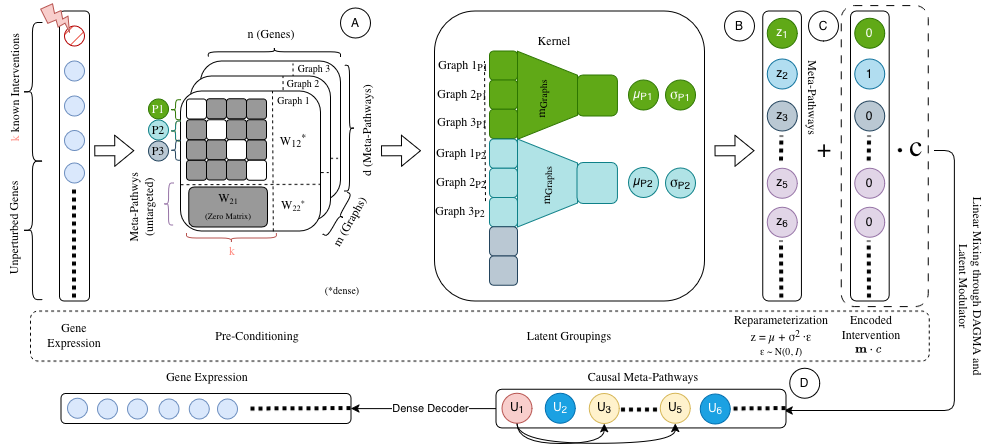
\includegraphics[width=\linewidth]{gfx/GraphPathway_modified.png}
    \caption{
        \textbf{The GraphPathway Encoder architecture of \gls{raptorgraph}.}
        \textbf{A}: \revised{Gene expression of control cells ($\zobs$) is fed as input to} the preconditioned linear layer, \revised{which} enforces a sparse, one-to-one mapping for known perturbed genes \revised{to explicitly} prevent intervention spillover.
        \textbf{B}: \revised{Complex dependencies are captured by learning} multiple parallel graph representations, \revised{which are then} aggregated to model non-linear interactions.
        \textbf{C}: A standard \gls{vae} reparameterization head \revised{generates} the stochastic latent variables \revised{($\latentvars$)}.
        \textbf{D}: A \revised{Latent Modulator takes the perturbation label as input and applies} atomic perturbations \revised{($\effectvector$)} to the independent latents \revised{($\latentvars$), shifting the distribution from the observed latent state ($\zobs$) to the interventional latent state ($\zint$). Both $\zobs$ and $\zint$ are then transformed by the DAGMA layer} through the learned \gls{dag} via linear mixing to \revised{yield} the final causal states \revised{($\latentcausalvars$), which are reconstructed into the predicted control ($\hat{\variables}_{\text{obs}}$) and perturbed ($\hat{\variables}_{\text{int}}$) gene expression profiles by a dense decoder.}
    }
    \label{fig:arch:graphpathway_encoder}
\end{figure}

% \begin{figure}[htbp]
%     \centering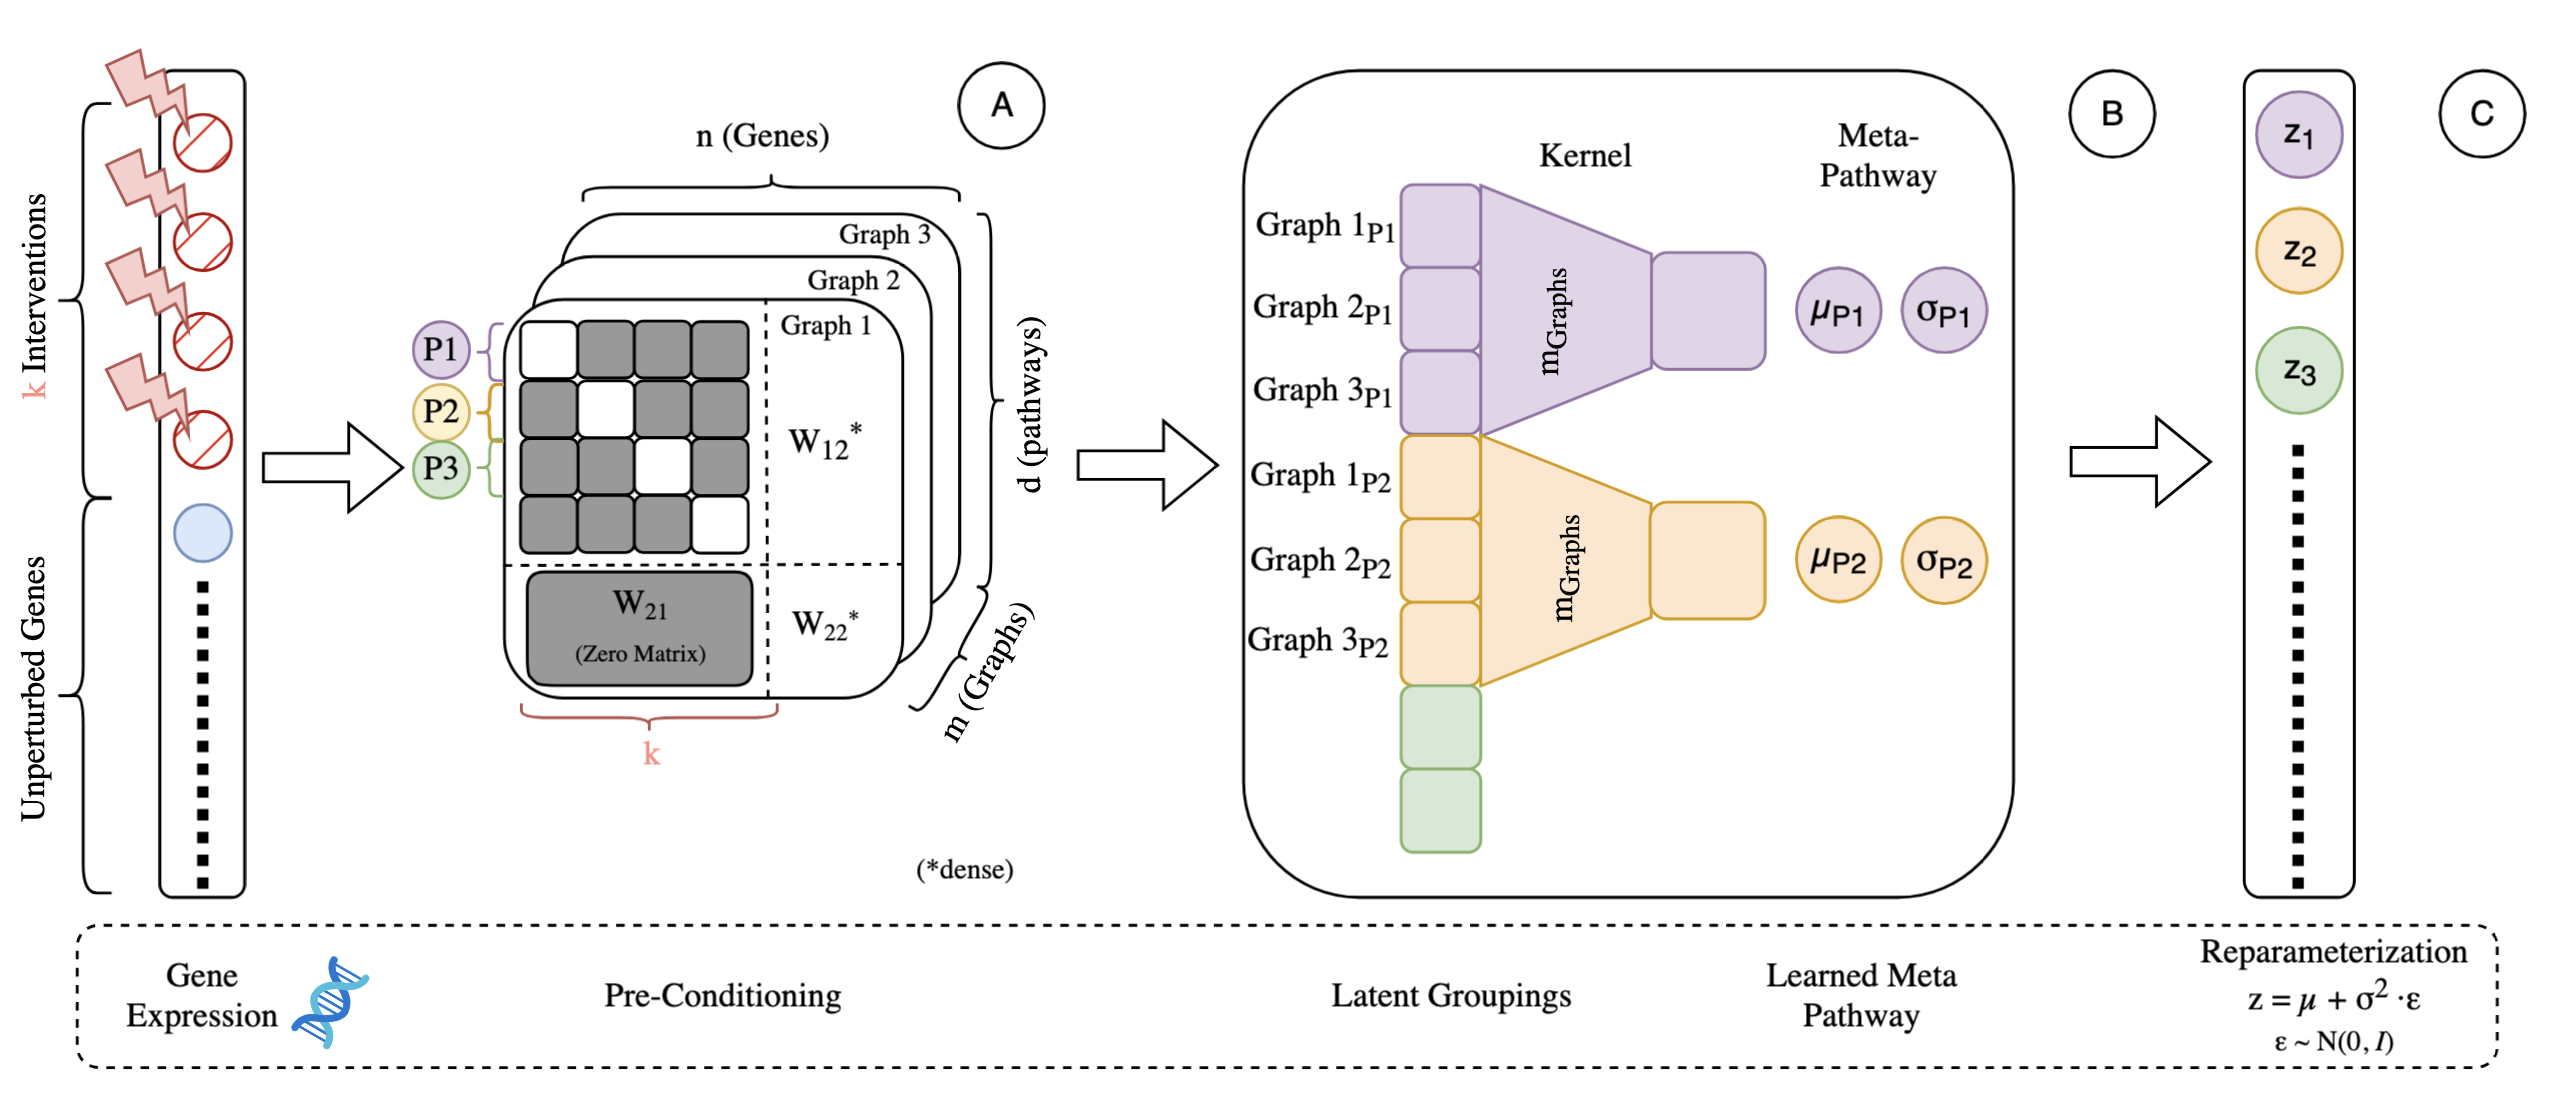
\includegraphics[width=1\linewidth]{gfx/GraphPathwayLayer_final.png}
%     \caption{
%         The GraphPathway Encoder architecture of \gls{raptorgraph}.
%         \textbf{A}: The preconditioned linear layer enforces a sparse, one-to-one mapping for known perturbed genes, preventing spillover.
%         \textbf{B}: Multiple parallel graph representations are learned and then aggregated to model non-linear interactions.
%         \textbf{C}: A standard \gls{vae} reparameterization head produces the final stochastic latent variables.
%     }\label{fig:arch:graphpathway_encoder}
% \end{figure}

%-------------------------------------------------------------------------------
% Subsection: Deep Causal Graph Learning with DAGMA
%-------------------------------------------------------------------------------
\subsection{Deep Causal Graph Learning with DAGMA}
\label{subsec:methods:dagma}
%-------------------------------------------------------------------------------

The GraphPathway Encoder with preconditioning fundamentally alters the causal structure discovery task.
By fixing the mapping  to specific latent variables, it eliminates the need for permutation-based discovery methods that assume a dense, entangled encoder.
However, this fixed ordering makes simple acyclicity constraints, such as enforcing an upper-triangular adjacency matrix, unsuitable.
These methods impose a strict and arbitrary causal hierarchy, as the influence of one latent variable on another is entirely restricted by their ordering (e.g., latent $i$ can only influence latent $j$ if $i<j$), which would conflict with the true biological relationships we aim to discover.
For this, we adapt the DAGMA framework~\citep{bello2022dagma} for its use in a deep learning context.

\textbf{DAGMA} reformulates the combinatorial search for a \gls{dag} into a continuous optimization problem.
This is achieved by minimizing a score function that measures data fit, subject to a differentiable constraint that is satisfied only if the graph is acyclic.
The DAGMA acyclicity constraint, $\acyclicityfunc_s(\graphmatrix)$, is based on a log-determinant function:
\begin{equation}
    \acyclicityfunc_s(\graphmatrix) = -\log\det(s\identitymatrix - \graphmatrix \circ \graphmatrix) + \latentdim\log s = 0
\end{equation}
where $\graphmatrix \in \realnumbers^{\latentdim \times \latentdim}$ is the weighted adjacency matrix of the latent graph, $s > 0$ is a scaling scalar, and $\circ$ represents the Hadamard product. Note that the condition holds if and only if $\graphmatrix$ represents a \gls{dag}.
The optimization then solves a sequence of unconstrained problems that jointly minimize a data-fit score and the acyclicity penalty.

%We implement a modified DAGMA approach with a dual-gradient system to ensure stability and causal fidelity.
%The causal graph is learned by computing the DAGMA loss exclusively on the latent representations of observational data.
%This encourages the model to learn the invariant, baseline causal structure of the biological system.
%Our implementation includes several key modifications for stable and effective graph discovery within a deep generative model.
\revised{\textbf{DAGMA implementation.} We implement a modified DAGMA approach designed to learn the invariant, baseline causal structure of the biological system.
To ensure stability and manage the trade-off between reconstruction fidelity and acyclicity, we introduce two critical regularization.
First, we employ a path-following schedule where the score weight $\mu$ is gradually decreased (see \cref{eq:dagma_loss_full}), allowing the model to prioritize feature learning early in training before strictly enforcing the graph constraint.
Second, we isolate gradient flow by computing the DAGMA-associated loss $\dagmaloss$ on detached latent representations.
This ensures the acyclicity constraint optimizes the graph structure without distorting the encoder's representation learning.}
A detailed description of the DAGMA layer, its objective, theoretical background, and implementation can be found in \cref{app:dagma}.

%===============================================================================
\subsection{Optimal Transport for Deterministic Interventional Learning}
%===============================================================================

A fundamental challenge in single-cell interventional modeling is the lack of direct one-to-one mappings between control and perturbed cells, creating a counterfactual gap.
Standard approaches often address this by randomly pairing control and interventional samples during training.
However, this random pairing matches cells with poor counterfactuals, providing inconsistent gradient signals that force the model to minimize loss by predicting the average of the target distribution---a phenomenon we term \textit{mean collapse} (see \cref{fig:app:ot_comparison}).
To resolve this, we employ a Wasserstein-based \gls{ot} framework to establish a deterministic, globally optimal mapping.
By minimizing the total transport cost between the control and perturbed populations, \gls{ot} pairs each cell with its most biologically similar counterpart.
This preserves heterogeneous subpopulation structures and ensures stable, structure-preserving representations for causal discovery.
Mathematical details are provided in \cref{app:ot}.

%-------------------------------------------------------------------------------
% Subsection: Training Objective
%-------------------------------------------------------------------------------
\subsection{Training Objective}
\label{subsec:methods:loss}
%-------------------------------------------------------------------------------

The model is trained end-to-end by minimizing a composite objective function, $\totalloss$, which balances four specialized components to ensure robust representation learning and causal discovery:
\begin{equation}
    \totalloss = \alpharec\mseloss + \betakl\kldloss +\quad \gammammd\mmdloss + \deltadagma\dagmaloss
    \label{eq:total_loss}
\end{equation}
where the scalar hyperparameters $\alpharec, \betakl, \gammammd$, and $\deltadagma$ balance each term's contribution. 
Specifically, we employ a reconstruction loss ($\mseloss$) to maintain high-fidelity control unperturbed cell reconstruction; 
a KL divergence ($\kldloss$) to regularize the meta-pathway manifold; 
an interventional prediction loss ($\mmdloss$) to align distributions of predicted perturbed gene expressions with those of the experimental ground truth; 
and a causal graph loss ($\dagmaloss$) to enforce structural acyclicity and data fit, defined as:
\begin{equation}
    \dagmaloss = \mu(\scorefunc(\graphmatrix; \datamatrix) + \lambda_1 \|\graphmatrix\|_1) + \acyclicityfunc(\graphmatrix)
    \label{eq:dagma_loss_full}
\end{equation}
where $\scorefunc(\graphmatrix; \datamatrix)$ is a score (see \cref{app:dagma:optimization}), $\|\graphmatrix\|_1$ is the L1 norm of the adjacency matrix, and $\acyclicityfunc(\graphmatrix)$ is the acyclicity penalty.
A comprehensive derivation and discussion of each term is provided in \cref{app:metrics}.


%\section{Experimental Settings}
%\label{sec:experiments}
%%===============================================================================
\subsection{Evaluation Setup, Metrics and Datasets}
\label{subsec:eval_setup_metrics}
%===============================================================================

To ensure a consistent and fair benchmark across all evaluated  models, we use \gls{mmd} to assess the similarity between predicted and true gene expression distributions.
The \gls{mmd} is calculated per type of perturbation (single or combinations thereof) and then averaged to provide an overall measure of distribution similarity.
Alongside objective metric comparison, we use Precision@10 to evaluate non-additive interactions of combinatorial perturbations (see \cref{app:metrics}).

For evaluation we use two datasets: First, the Perturb-seq single-cell RNA-seq dataset from~\citet{norman2019exploring} and as processed in the CPA study~\citep{lotfollahi2023predicting} and refer to it as the Norman-CPA dataset.
It profiles 105 gene perturbations in K562 cells, including both single and double perturbations.
In total, 284 conditions across $\sim$108,000 cells were measured, of which 131 represent unique gene–gene combinations and the remaining 153 represent single perturbations. For each perturbation, associated control cells were also profiled. 
We utilize the entire set of single-perturbations during training and evaluate the subsequent methods on the double-perturbations.

Additionally, we used the CRISPRi single-cell RNA-seq dataset curated by~\citet{replogle_combinatorial_2020} and as processed in the PerturBase study~\citep{wei_perturbase_2024}. We refer to it as the Replogle2020 dataset.
This dataset profiles 82 gene perturbations in K562 cells, including both single (44), double perturbations (37), and control.
The 82 conditions were measured across $\sim$22,740 cells.

\section{Experiments}
\label{sec:results}
%===============================================================================
\section{Experiments}
\label{sec:results}
%===============================================================================
\subsection{Evaluation Setup, Metrics and Datasets}
\label{sec:results:setup}
%===============================================================================
\textbf{Datasets.} For evaluation, we use two datasets: First, the Perturb-seq single-cell RNA-seq dataset from~\citet{norman2019exploring} and as processed in the CPA study~\citep{lotfollahi2023predicting} and refer to it as the Norman-CPA dataset.
It profiles 105 gene perturbations in K562 cells, including both single and double perturbations.
In total, 284 conditions across $\sim$108,000 cells were measured, of which 131 represent unique gene–gene combinations and the remaining 153 represent single perturbations. For each perturbation, associated control cells were also profiled. 
We utilize the entire set of single-perturbations during training and evaluate the subsequent methods on the double-perturbations.

Additionally, we used the CRISPRi single-cell RNA-seq dataset curated by~\citet{replogle_combinatorial_2020} and as processed in the PerturBase study~\citep{wei_perturbase_2024}. We refer to it as the Replogle2020 dataset.
This dataset profiles 82 gene perturbations in K562 cells, including both single (44), double perturbations (37), and control.
The 82 conditions were measured across $\sim$22,740 cells.

\textbf{Benchmarked models.} We benchmark \gls{raptorgraph} generative performance against four state-of-the-art models: SENA, scGPT, \gls{dvae}, and GEARS.
We start by assessing two key aspects of prediction fidelity using the single-cell perturbation dataset from \citet{norman2019exploring}.
\revised{We prioritized the Norman-CPA dataset for this comprehensive quantitative benchmarking because the implementations of several baseline models have auxiliary files and preprocessing steps that are tightly coupled to it, making adaptation to other datasets non-trivial.
However, to further demonstrate generalizability, we provide an additional evaluation on the Replogle2020 dataset, restricted to a comparison between \gls{raptorgraph} and scGPT.}

\textbf{Evaluation Metrics.} To ensure a consistent and fair benchmark across all evaluated models, we use \gls{mse} and \gls{mmd} to assess the similarity between predicted and true gene expression distributions.
The \gls{mmd} is calculated per type of perturbation (single or combinations thereof) and then averaged to provide an overall measure of distribution similarity.
Alongside objective metric comparison, we use Precision@10 to evaluate non-additive interactions of combinatorial perturbations (see \cref{app:metrics}).

\subsection{Hyperparameter ablation studies} 
\revised{
To validate our hyperparameter selection, we conducted a comprehensive ablation study on the VAE regularization parameter ($\beta$) and the DAGMA score weights ($\mu, \lambda_1$).
Our analysis reveals a critical trade-off between distribution matching and the preservation of biological heterogeneity.
See \cref{app:extended_results:ablation_study} for detailed results of the full hyperparameter sweep and the rationale for the selected configuration.}
%
\subsection{Learning capabilities of \gls{raptorgraph}} First, we measured the MSE between the ground truth and predicted profiles of control cells to evaluate how well each model reconstructs the basal, unperturbed cellular state.
Second, we calculated the \gls{mmd} between the distributions of ground truth and predicted profiles for double-gene perturbations to assess the model's ability to capture the global transcriptional shift following a complex intervention. A detailed description of these metrics is provided in \cref{app:metrics}. 

\begin{table}[htb]
    \centering
    \caption{Results using the Norman-CPA dataset are averaged over $3$ runs. Bold: best results; Italics: second best. \revised{Values are mean $\pm$ variance.} 
    *We excluded the GEARS model because it behaves in a fundamentally different way that is incompatible with our evaluation framework, making a fair and direct comparison impossible (see \cref{app:metrics:gears_exclusion}).}
    \label{tab:MMD_results}
    \vskip 0.15in
    \begin{center}
    \begin{small}
    \resizebox{\columnwidth}{!}{%
    \begin{tabular}{lccccc}
        \toprule
        {Metric} & {SENA} & {scGPT} & {\gls{dvae}} & {GEARS} & {\gls{raptorgraph}} (ours) \\
        \midrule
        \gls{mmd} & 0.522 $\pm$ 0.003 & 0.176 $\pm$ 0.001 & \textbf{0.076 $\pm$ 0.000} & {--}* & {\textit{0.112 $\pm$ 0.001}} \\
        \gls{mse} & \textbf{0.043 $\pm$ 0.000} & 0.066 $\pm$ 0.000 & 0.062 $\pm$ 0.000 & {--}* & {\textit{0.045 $\pm$ 0.000}} \\
        \bottomrule
    \end{tabular}
    }
    \end{small}
    \end{center}
    \vskip -0.1in
\end{table}

The results in \Cref{tab:MMD_results} highlight a crucial trade-off between reconstruction fidelity (\gls{mse}) and distributional accuracy (\gls{mmd}).
\Gls{raptorgraph} achieves a strong overall balance, demonstrating highly competitive performance across both reconstruction and generative capabilities. 

\revised{The additional benchmark using the Repogle2020 dataset (shown in \Cref{tab:objective_results_replogle} and restricted to a direct comparison between \gls{raptorgraph} and scGPT) further demonstrates our model's robust performance and superior reconstruction fidelity on independent biological data.}

\begin{wraptable}{r}{0.48\textwidth}
    \centering
    \vspace{-6pt}
    \vspace{-0.5\baselineskip}
    \caption{\revised{Results using the Replogle2020 dataset are averaged over $3$ runs. Values are mean $\pm$ variance. Bold: best results.}}
    \resizebox{0.48\textwidth}{!}{%
    \begin{tabular}{lcc}
        \toprule
        {Metric} & {scGPT} & RAPTORGraph (ours) \\
        \midrule
        \gls{mmd} & 0.138 $\pm$ 0.000 & \textbf{0.137 $\pm$ 0.000} \\
        \gls{mse} & 0.069 $\pm$ 0.000 & \textbf{0.054 $\pm$ 0.000} \\
        \bottomrule
    \end{tabular}%
    }
    \label{tab:objective_results_replogle}
    \vspace{-\baselineskip}
\end{wraptable}

\subsection{Prediction of non-additive genetic perturbations.} 
%This complex and biologically significant benchmark 
We next assess model's ability to predict complex interaction effects between single-gene perturbations beyond simple linear combinations  (\Cref{tab:gi_scores}).
Specifically, we compared each model based on its ability to predict five distinct interaction types, using Precision@10 to quantify how effectively each model could identify true interactions within its top 10 predictions, a direct measure of its utility for experimental discovery (see \cref{app:metrics:genetic_interaction}). \gls{raptorgraph} is among the top performers in almost all metrics, yielding the best overall performance across all methods.  

\begin{table}[htb]
\centering
\caption{Comparison of non-additive genetic interaction prediction. Precision@10 scores for five baseline models across distinct genetic interaction subtypes on the Norman et al. dataset. Higher is better. Bold: best results; Italics: second best.\revised{Values are mean $\pm$ variance over 3 runs.}}
\label{tab:gi_scores}
\vskip 0.15in
\begin{center}
\begin{small}
\resizebox{\columnwidth}{!}{%
\csvreader[
    separator=comma,
    tabular= lccccc,
    table head=\toprule Metric & \gls{dvae} & SENA & GEARS & scGPT & \gls{raptorgraph} (ours)\\\midrule,
    late after line=\\, 
    table foot=\bottomrule
]{results_files/gi_scores/precision_at_10_summary_transposed.csv}{type=\Metric,scGPT=\scGPT,dvae=\dvae,raptor=\raptor,sena=\sena,gears=\gears}
{\Metric & \dvae & \sena & \gears & \scGPT & \raptor}
}
\end{small}
\end{center}
\vskip -0.1in
\end{table}

\textbf{OT ablation study.} We further investigated the contribution of \gls{ot} to this performance. Our ablation study reveals that \gls{ot} preprocessing is a key driver of the model's ability to predict complex non-additive interactions, particularly boosting redundancy and epistasis. Importantly, \gls{ot}-based pairing significantly outperforms a random pairing baseline. Note that this benefit comes with negligible computational overhead ($\approx 2.2\%$ of total training time). See \cref{app:extended_results:ot_impact} and \cref{app:extended_results:ot_complexity} for further details.
%Detailed analyses of these empirical benefits and the computational cost are provided in \cref{app:extended_results:ot_impact} and \cref{app:extended_results:ot_complexity}, respectively.

\subsection{Reverse Perturbation Analysis} 

\begin{wrapfigure}[17]{r}{0.6\textwidth}
\vspace{-20pt}
    \centering
    \vspace{-0.75\baselineskip}
    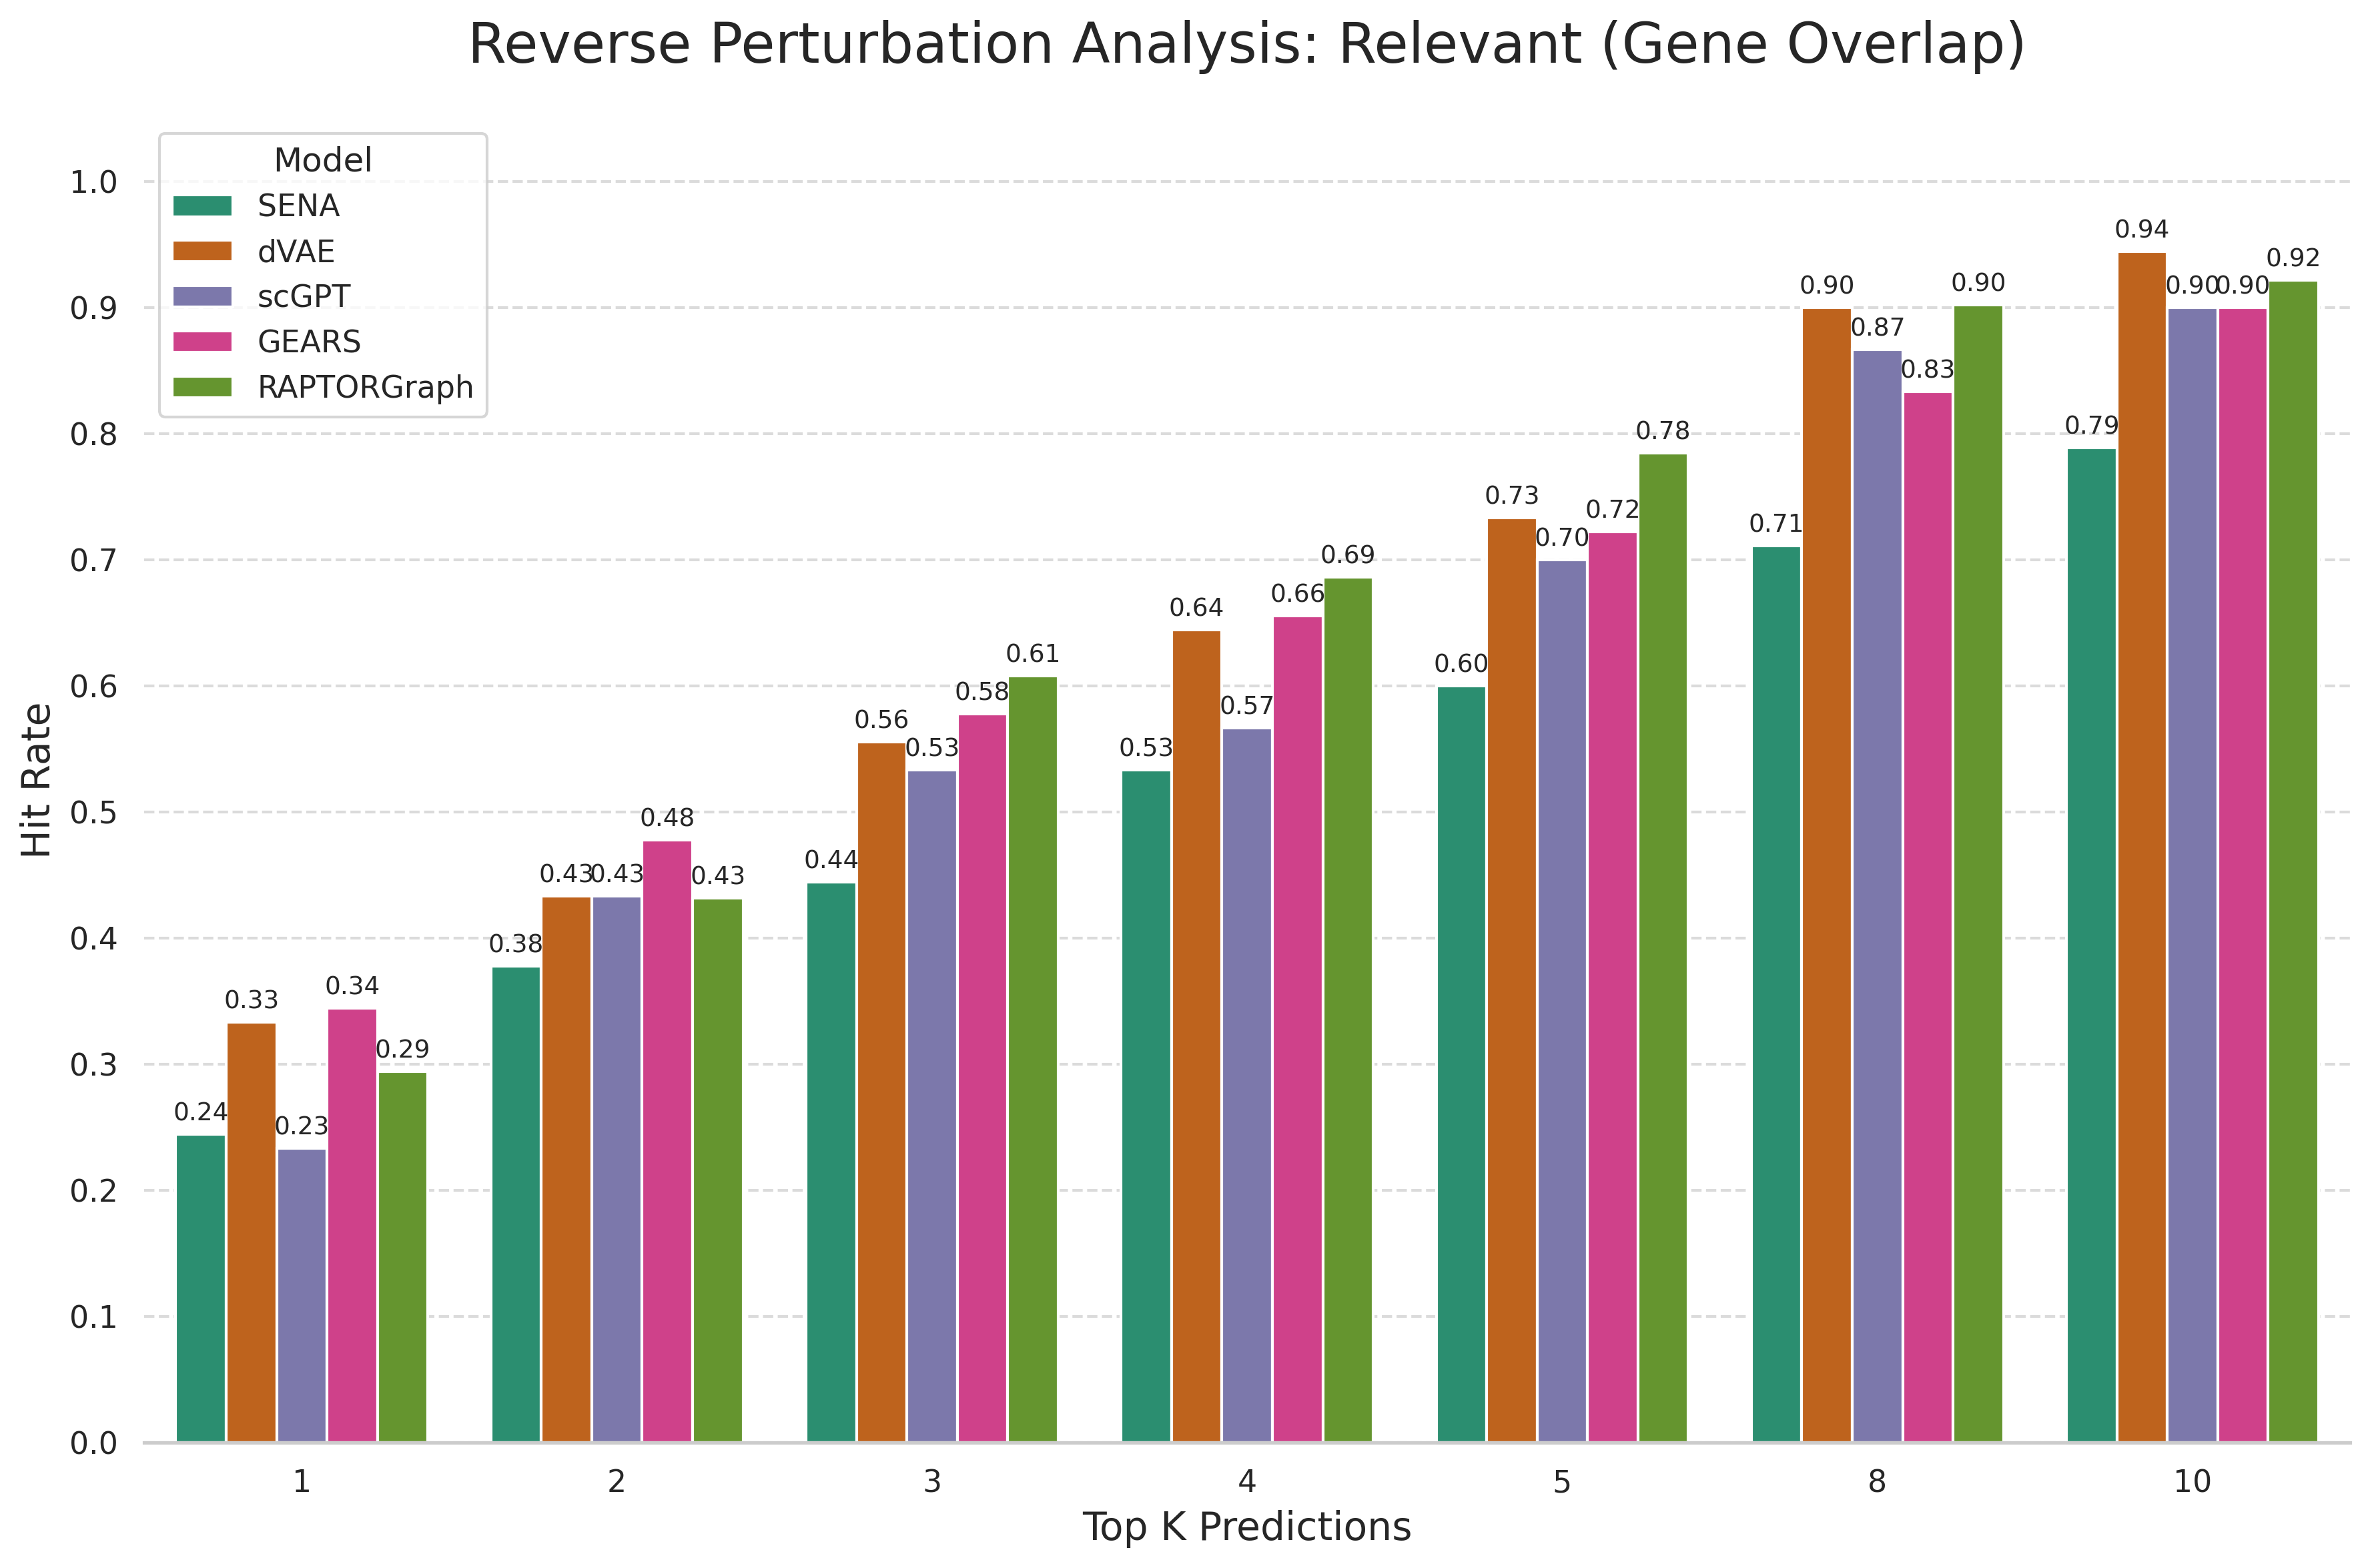
\includegraphics[width=0.98\linewidth]{gfx/results/hit_rate_at_k_relevant_gene_overlap.png}
    \caption{Hit Rate @ K (averaged over 3 runs).
    The metric measures the fraction of queries where at least one correct gene was identified in the top K predictions.
    Higher is better.}
    \label{fig:app:hit_rate_relevant}
    \vspace{-\baselineskip}
\end{wrapfigure}
While predicting genetic interactions demonstrates a model's forward predictive power, a more profound test is its ability to reverse-engineer the genetic cause of an observed phenotype.
To this end, we challenged a model to identify the specific genetic perturbation responsible for a given cellular gene expression profile.
The analysis was performed on a controlled combinatorial space of 20 transcription factors from the \citet{norman2019exploring} dataset.
For each model, we generated a database of predicted expression profiles for all possible double-gene perturbations within this subset.
We then used the ground truth mean expression profiles from experimentally observed double perturbations as queries, ranking the database entries by similarity to identify the most likely causal perturbation.

We first evaluated the models on the highly stringent task of identifying the exact causal gene combination, quantified by the Correct (Exact Match) Hit Rate @ K.
As shown in \cref{fig:app:hit_rate_exact}, all models achieve modest hit rates, underscoring the profound difficulty of this reverse-engineering challenge.

However, a more practical measure of a model's utility to guide experimental genetic perturbation designs is its ability to retrieve perturbations containing at least one of the correct genes. We thus evaluated each model's capacity to identify biologically influential genes using the Relevant (Gene Overlap) Hit Rate @ K (see \cref{fig:app:hit_rate_relevant} and \Cref{tab:hit_rate}).



\Gls{raptorgraph}  demonstrates exceptional performance, consistently ranking among the top models.
This highlights that while pinpointing exact higher-order interactions is an ongoing challenge, \gls{raptorgraph} is highly effective at identifying the key genetic players driving a cellular response, making it a highly valuable tool for hypothesis generation and experimental design.
\begin{table}[htb]
\centering
\caption{
    Hit Rate @ K (relevant) for the reverse perturbation task.
    The metric measures the fraction of queries where at least one correct gene was identified in the top K predictions.
    Higher values are better.
    \revised{Values are mean $\pm$ variance over 3 runs.}
}
\label{tab:hit_rate}
\vskip 0.15in
    \begin{center}
    \begin{small}
    \resizebox{\columnwidth}{!}{%
    \csvreader[
        separator=comma,
        tabular= lccccc,
        table head=\toprule $k$ & \gls{dvae} & SENA & GEARS & scGPT & \gls{raptorgraph} (ours)\\ \midrule,
        late after line=\\, 
        table foot=\bottomrule
    ]{results_files/hit_rate/hit_rate_at_k_summary_transposed.csv}{k=\k,SENA=\SENA,scGPT=\scGPT,dVAE=\dVAE,GEARS=\GEARS,RAPTORGraph=\RAPTORGraph}
    {\k & \dVAE & \SENA & \GEARS & \scGPT & \RAPTORGraph}
    }
    \end{small}
    \end{center}
\vskip -0.1in
\end{table}


\section{\revised{\gls{raptorgraph} learns biologically meaningful \cmps{}}}

\revised{To confirm that \gls{raptorgraph} learns biologically meaningful causal structures rather than arbitrary representations, we examined the functional identity of the \cmps{} using Gene Set Enrichment Analysis (GSEA).
For each \cmp{}, we identify the $N$ single-gene interventions that induce the greatest change in that meta-pathway.
Then, for every such ranked gene list, we perform a GSEA to identify significantly enriched biological processes (also known as pathways) within this set of $N$ genes, serving as transcriptional signatures for the causal meta-pathway. It is important to differentiate between the GSEA-derived pathways (which are well-described biological processes from known databases) and the causal meta-pathways (which are learned causal latent factors that are associated with single interventions). Thus, our goal here is to assess whether the learned causal meta-pathways encompass relevant and related biological processes.
For this evaluation, we use the ``Hallmark'' gene sets from the Human Molecular Signatures Database (MSigDB) database~\citep{liberzon_molecular_2015}.}
%We observed a robust alignment between the known biological roles of perturbed genes and the pathway enrichments of their corresponding \cmps{}.

\revised{The GSEA analysis reveals that \gls{raptorgraph} captures distinct and biologically accurate programs. \Cref{fig:app:pathway_heatmap_supp} visualizes the Normalized Enrichment Scores (NES) for the top enriched pathways across the learned factors. We highlight distinct biological programs captured by the model, verified against the known functions of their corresponding gene perturbations:}
%
\begin{enumerate}[leftmargin=*]
     \item \revised{\textbf{Differentiation-Induced Arrest:} The \cmp{} linked to \textit{EGR1} displays massive negative enrichment for ``E2F Targets'' and ``G2-M Checkpoint''.
    EGR1 is a known tumor suppressor in K562 leukemia cells that drives differentiation along the megakaryocytic lineage, a process that necessitates a complete exit from the cell cycle \citep{ma_emodin_2019}.
    \gls{raptorgraph} correctly identifies this potent anti-proliferative program.}
    \item \revised{\textbf{Stress-Induced Growth Arrest:} The \cmp{} linked to the AP-1 subunit \textit{JUN} shows strong negative enrichment for ``E2F Targets'' and ``G2-M Checkpoint''. While often associated with inflammation, c-Jun is a central stress-response mediator; in the context of K562 cells, its activation drives a termination of cell division required for stress adaptation or differentiation \citep{shaulian_ap-1_2002, shaulian_mammalian_2000}.}
    \item \revised{\textbf{p53-Like Tumor Suppression:} The \cmp{} associated with \textit{TP73} displays significant negative enrichment for ``G2-M Checkpoint''.
    \textit{TP73} is a functional homolog of \textit{TP53} (p53); its activation triggers downstream checkpoint signaling that arrests the cell cycle to prevent genomic instability \citep{kaghad_monoallelically_1997}.}
\end{enumerate}
%
\revised{
These findings confirm that the nodes in our learned DAG represent specific biological mechanisms and that the edges learned by the DAGMA module can be interpreted as causal regulatory links between these verified biological processes. A detailed description of the methodology is provided in \cref{app:metrics:gsea_setup}.
}
%
Detailed GSEA results and the associated enrichment heatmap are provided in \cref{app:extended_results:biological_validation}.

%===============================================================================
\section{Conclusion and Limitations}
\label{sec:conclusion}
%===============================================================================

Developing interpretable \emph{in silico} models is crucial for therapeutic discovery, yet current approaches face two key challenges: intervention spillover, where dense encoders create entangled latent signals that confound causal discovery, and mean collapse, where the absence of one-to-one cell pairings erodes cellular diversity. We introduce \gls{raptorgraph}, a framework that directly resolves these issues. To counteract intervention spillover, it combines a preconditioned GraphPathway layer, enforcing the sparse mappings required for clean single-node interventions, with a DAGMA layer for robust DAG discovery.
\revised{This architectural design eliminates the artifactual entanglement of input genes with latent pathways, while the subsequent DAG module explicitly learns the legitimate biological causal relationships and correlations between the resulting sparse pathway activities.}
To prevent mean collapse, \gls{raptorgraph} globally pairs control and perturbed populations through \gls{ot}.
\gls{raptorgraph} not only achieves a superior balance between reconstruction fidelity and distributional accuracy compared to state-of-the-art methods, but also demonstrates a superior capability to predict complex, non-additive genetic interactions, and can reverse-engineer genetic drivers to generate testable hypotheses.
\gls{raptorgraph} bridges predictive power and mechanistic insight, enabling not only the prediction of a perturbation's effect but also understanding the reasoning behind it.

\paragraph{Limitations.}
While \gls{raptorgraph} significantly advances interpretable causal discovery, several limitations remain. 
First, the framework is primarily optimized for atomic genetic interventions (e.g., CRISPRa/i), where each intervention has a clear, primary target. 
In contrast, chemical or drug perturbations often exhibit complex multi-target profiles or off-target effects that may not map as cleanly to a single node in our GraphPathway encoder. 
Second, the current implementation focuses on transcriptomic readouts; extending \gls{raptorgraph} to multi-omic interventional data (e.g., Perturb-ATAC-seq) to capture the interplay between epigenetic regulatory states and gene expression is a promising direction for future research.

Future work will focus on deploying \gls{raptorgraph} for the hypothesis-driven discovery of novel drug targets and exploring its utility in uncovering cell-type specific pathway mechanisms.
% Future work will focus on deploying \gls{raptorgraph} for the hypothesis-driven discovery of novel drug targets and exploring its utility in uncovering cell-type specific pathway mechanisms.

% The development of predictive and causally-aware \textit{in silico} models is critical for advancing therapeutic discovery and our fundamental understanding of biology.
% However, current approaches for predicting cellular responses face two key challenges.
% First, many predictive models act as uninterpretable ``black boxes'', while \gls{crl} models that use dense encoders are forced to identify a discrete intervention target from an entangled latent signal, a task which introduces unnecessary complexity and leads to suboptimal solutions, which we term as \emph{intervention spillover}.
% Second, learning from single-cell data is challenging due to the absence of a one-to-one mapping between control and perturbed cell populations, and random pairing strategies lead to \emph{mean collapse}, a phenomenon where the model learns an average response that erodes cellular diversity.

% In this work, we introduced \gls{raptorgraph}, a framework designed to bridge this gap by directly addressing two critical issues.
% First, we solve the \emph{intervention spillover} problem through a combination of preconditioned GraphPathway and DAG discovery based on the DAGMA layer.
% Our novel GraphPathway layer addresses this by using preconditioning to enforce sparse gene-to-\cmp{} mappings, enabling the clean, single-node interventions required for valid causal inference.
% Our DAGMA layer solves the problem where the order causal latent variables are fixed, which render simple acyclicity constraints, such as enforcing an upper-triangular adjacency
% matrix, unsuitable.
% Second, we address the \emph{mean collapse} problem by employing an \gls{ot}-based preprocessing step to globally pair the control samples with intervened samples.
% Our empirical evaluation demonstrates the effectiveness of this approach. 
% \Gls{raptorgraph} achieves a superior overall performance by providing a strong balance between reconstruction fidelity and distributional prediction accuracy.
% Furthermore, it excels at predicting complex, non-additive genetic interactions and demonstrates a strong capacity for reverse-engineering the genetic drivers of a given cellular phenotype, highlighting its utility for generating testable hypotheses.

%---------------------------------------------------------------------
% Broader Impact Statement
%---------------------------------------------------------------------
\section*{Broader Impact Statement}
This paper presents work whose goal is to advance the field of Machine Learning by improving the interpretability and accuracy of causal discovery in biological systems. 
By enabling more precise \insilico{} predictions of genetic perturbations, our framework potentially accelerates therapeutic discovery and reduces the need for exhaustive experimental screening. 
While the primary focus is on basic research in cellular biology, we recognize that improved causal modeling of biological data could eventually inform clinical decision-making; thus, we emphasize the importance of independent experimental validation before applying these findings in medical contexts. 
There are no direct negative societal consequences of this work anticipated at this stage.

%---------------------------------------------------------------------
% Bibliography
%---------------------------------------------------------------------
\bibliography{raptor_references}
\bibliographystyle{plainnat}

%---------------------------------------------------------------------
% Appendix
%---------------------------------------------------------------------
\newpage
\appendix
\onecolumn
\newpage
\appendix
\setcounter{equation}{0}
\renewcommand{\theequation}{S\arabic{equation}}
\renewcommand{\theHequation}{S\arabic{equation}}
\glsresetall

\clearpage

%===============================================================================
% 			PREFIX ALL APPENDIX FIGURES/TABLES WITH 'S'
%===============================================================================
\renewcommand{\thefigure}{S\arabic{figure}}
\renewcommand{\thetable}{S\arabic{table}}
%===============================================================================

%-------------------------------------------------------------------------------
% I. DEFINITIONS AND BACKGROUND
%-------------------------------------------------------------------------------
%===============================================================================
%  APPENDIX: NOMENCLATURE
%===============================================================================
\section{Nomenclature and Mathematical Notation}
\label{app:nomenclature}
%===============================================================================

In this section, we provide a comprehensive list of the mathematical notations used throughout our work, organized by category.
This serves as a centralized reference to ensure clarity and consistency.

%-------------------------------------------------------------------------------
\subsection{General Variables and Data Structures}
\label{app:nomenclature:general}
%-------------------------------------------------------------------------------

We begin by defining the fundamental variables and data structures used to represent observed and latent spaces.

\begin{table}[H]
\begin{tabularx}{\textwidth}{l X}
\toprule
\textbf{Symbol} & \textbf{Description} \\
\midrule
$\realnumbers$ & The set of real numbers. \\
$\variables$ & A vector of observed variables (e.g., gene expression). \\
$\latentvars$ & A vector of general latent variables in the learned representation space. \\
$\noiseterms$ & A vector of general, unspecified noise terms. \\
$\datamatrix$ & A matrix representing a set of observed data samples. \\
$\identitymatrix$ & The identity matrix. \\
\bottomrule
\end{tabularx}
\end{table}

%-------------------------------------------------------------------------------
\subsection{Causal Models and Graphs}
\label{app:nomenclature:causal}
%-------------------------------------------------------------------------------

Next, we define the components of the Structural Causal Model (SCM) that describes the underlying data-generating process.

\begin{table}[H]
\begin{tabularx}{\textwidth}{l X}
\toprule
\textbf{Symbol} & \textbf{Description} \\
\midrule
$\graph$ & A \gls{dag} representing the causal structure. \\
$\graphmatrix$ & The weighted adjacency matrix of the causal graph $\graph$. \\
$\adjacencymatrix$ & A general adjacency matrix. \\
$\weightmatrix$ & A general weight matrix. \\
$\parentnodes(\cdot)$ & A function that returns the parent nodes of a given node in $\graph$. \\
$\transitiveclosure{\graph}$ & The transitive closure of the graph $\graph$. \\
$\latentcausalvars$ & The true, unobserved latent causal variables in the \gls{scm}. \\
$\latentcausalvar$ & A single latent causal variable. \\
$\exonoise$ & A vector of exogenous noise terms for the \gls{scm}. \\
$\structuralfunc_i$ & The structural causal function for a single variable $\latentcausalvar_i$. \\
$\tr(\cdot)$ & The trace function for a matrix. \\
\bottomrule
\end{tabularx}
\end{table}

%------------------------------------------------------------------------------
\subsection{Model Functions and Representations}
\label{app:nomenclature:model_functions}
%------------------------------------------------------------------------------

We denote the core functions of our model, which learn to map between the observed and latent spaces, as follows.

\begin{table}[H]
\begin{tabularx}{\textwidth}{l X}
\toprule
\textbf{Symbol} & \textbf{Description} \\
\midrule
$\truemixingfunc$ & The true, unknown data-generating (mixing) function. \\
$\decoder$ & The learned decoder network. \\
$\idealencoder$ & The ideal, oracle encoder function. \\
$\practicalencoder$ & The practical, parameterized encoder network. \\
$\learnedrepresentation$ & The learned latent representation, output of the encoder ($\practicalencoder(\variables)$). \\
$\predictedvariable$ & A single data sample generated by the model's decoder. \\
$\predicteddatamatrix$ & A matrix representing a batch of data samples generated by the model's decoder. \\
$\composedfunc$ & The composed function $\practicalencoder \circ \truemixingfunc$. \\
$\latentideal$ & The true latent representation produced by the $\idealencoder$. \\
$\latentchangeideal$ & The ideal, single-node change in the latent space. \\
$\latentchangeapprox$ & The approximated (dense) change in the latent space. \\
$\normaldist$ & The normal (Gaussian) distribution. \\
%$\auxvar$ & An auxiliary conditioning variable (Khemakhem et al., 2020). \\
%$a$ & The composed function, $\practicalencoder \circ \truemixingfunc$. \\
%$p$ & The degree of a polynomial mixing function. \\
\bottomrule
\end{tabularx}
\end{table}

%-------------------------------------------------------------------------------
\subsection{Intervention-Specific Variables}
\label{app:nomenclature:interventions}
%-------------------------------------------------------------------------------

Here, we list the variables specifically related to the modeling of interventions.

\begin{table}[H]
\begin{tabularx}{\textwidth}{l X}
\toprule
\textbf{Symbol} & \textbf{Description} \\
\midrule
$\interventionencoder$ & The intervention encoder network. \\
$\vi$ & The one-hot vector specifying the target of an intervention. \\
$\conditionvector$ & A general condition vector input to an intervention network. \\
$\maskvector$ & The mask vector specifying an intervention's target(s). \\
$\interventionstrength$ & The scalar strength of a latent intervention. \\
$\zobs$ & Latents from an observational (control) sample. \\
$\zint$ & Latents from an interventional sample. \\
$\interventionaldist$ & The interventional distribution over latent variables. \\
$\interventionset$ & The set of intervened variables in environment $k$. \\
$\interventiontargets$ & The targets of an intervention for a variable $i$. \\
$\auxvar$ & An auxiliary variable providing conditioning information (e.g., environment index). \\
\bottomrule
\end{tabularx}
\end{table}

%-------------------------------------------------------------------------------
\subsection{Identifiability and Transformations}
\label{app:nomenclature:identifiability}
%-------------------------------------------------------------------------------

We define symbols used in the context of identifiability proofs and the resulting transformation classes.

\begin{table}[H]
\begin{tabularx}{\textwidth}{l X}
\toprule
\textbf{Symbol} & \textbf{Description} \\
\midrule
$\simT$ & Equivalence class for a transformation T. \\
$\simC$ & Equivalence class for a transformation C. \\
$\affinetransform$ & The matrix component of an affine transformation. \\
$\affineoffset$ & The vector component of an affine transformation. \\
$\scalefactor$ & A scalar factor in a scaling transformation. \\
$\shiftoffset$ & An offset in a shift transformation. \\
\bottomrule
\end{tabularx}
\end{table}

%-------------------------------------------------------------------------------
\subsection{Probability, Losses, and Functions}
\label{app:nomenclature:probability_losses}
%-------------------------------------------------------------------------------

We define the probability functions, loss functions, and mathematical operators used to train our models and enforce constraints.

\begin{table}[H]
\begin{tabularx}{\textwidth}{l X}
\toprule
\textbf{Symbol} & \textbf{Description} \\
\midrule
$\prob{\cdot}$ & \gls{pmf} (for discrete variables). \\
$\pdf{\cdot}$ & \gls{pdf} (for continuous variables). \\
$\cdf{\cdot}$ & \gls{cdf}. \\
$\pdata$ & The true, underlying data-generating distribution (\gls{pdf}). \\
$\pmodel$ & The learned distribution of the model (\gls{pdf}). \\
$\E[\cdot]$ & The expectation function. \\
$\dagmaloss$ & Loss function related to the causal graph structure. \\
$\mmdloss$ & Loss function based on the \gls{mmd}. \\
$\acyclicityfunc$ & A function used to enforce graph acyclicity. \\
$\scorefunc$ & A score function for graph discovery. \\
$\mmd(\cdot, \cdot)$ & The \gls{mmd} function, which computes the distance between two distributions. \\
$\mkmmd(\cdot, \cdot)$ & The \gls{mmd} function, which computes the distance between two distributions. \\
$\kernel(\cdot, \cdot)$ & A kernel function used in \gls{mmd} computation. \\
\bottomrule
\end{tabularx}
\end{table}

%-------------------------------------------------------------------------------
\subsection{Hyperparameters}
\label{app:nomenclature:hyperparams}
%-------------------------------------------------------------------------------

We list the key hyperparameters that control our model's training and behavior.

\begin{table}[H]
\begin{tabularx}{\textwidth}{l X}
\toprule
\textbf{Symbol} & \textbf{Description} \\
\midrule
$\scorelambda$ & Regularization hyperparameter for a graph score. \\
$\mmdsigmaMMD$ & The bandwidth hyperparameter for the Gaussian RBF kernel. \\
$\mkmmdweights$ & The weights for the convex combination in multi-kernel MMD. \\
$\numkernels$ & The number of kernels used in the \gls{mmd} calculation. \\
$\numgraphs$ & The number of graphs. \\
$\numsamplesobs$ & The number of samples in a batch of observed data. \\
$\numsamplespred$ & The number of samples in a batch of predicted data. \\
\bottomrule
\end{tabularx}
\end{table}

%-------------------------------------------------------------------------------
\subsection{Downstream Analysis Metrics}
\label{app:nomenclature:downstream_metrics}
%-------------------------------------------------------------------------------

We define variables used in the downstream evaluation tasks, such as the genetic interaction analysis.

\begin{table}[H]
\begin{tabularx}{\textwidth}{l X}
\toprule
\textbf{Symbol} & \textbf{Description} \\
\midrule
$\effectvector$ & The perturbation effect vector (mean of perturbed minus mean of control). \\
$\effectvectornaive$ & The naive additive effect vector, defined as $\effectvector A + \effectvector B$. \\
$\ltwonorm{\cdot}$ & The L2 norm of a vector. \\
$\cossim{\cdot}{\cdot}$ & The cosine similarity between two vectors. \\
$\meanexpression$ & The mean expression profile of a cell population. \\
$\numcells$ & The number of cells for a given perturbation condition. \\
$\predictionfunc_M$ & The prediction function for a given model $M$. \\
$\synergyscore$ & The score used to measure synergy and suppression. \\
$\neomorphismscore$ & The score used to measure neomorphism. \\
$\redundancyscore$ & The score used to measure redundancy. \\
$\epistasiscore$ & The score used to measure epistasis. \\
\bottomrule
\end{tabularx}
\end{table}

%-------------------------------------------------------------------------------
\subsection{Dimensionality and Spaces}
\label{app:nomenclature:dims}
%-------------------------------------------------------------------------------

Finally, we list symbols for dimensionality and the properties of the data spaces.

\begin{table}[H]
\begin{tabularx}{\textwidth}{l X}
\toprule
\textbf{Symbol} & \textbf{Description} \\
\midrule
$\observeddim$ & The dimensionality of the observed data space. \\
$\latentdim$ & The dimensionality of the latent space. \\
$\numpathways$ & The number of learned pathways, equivalent to $\latentdim$. \\
$\polydegree$ & The degree of a polynomial mixing function. \\
$\latentsupport$ & The support of the latent distribution. \\
$\observsupport$ & The support of the observed distribution. \\
$\numgenes$ & The number of genes in the expression profile, equivalent to $\observeddim$. \\
\bottomrule
\end{tabularx}
\end{table}

%-------------------------------------------------------------------------------
\subsection{Acronyms and Abbreviations}
\label{app:nomenclature:acronyms}
%-------------------------------------------------------------------------------

\printglossary[type=\acronymtype,title={List of Acronyms}]

\clearpage
%===============================================================================
% APPENDIX: MATHEMATICAL PROOFS AND THEORETICAL BACKGROUND
%===============================================================================
\section{Mathematical Proofs and Theoretical Background}
\label{app:proofs}
%===============================================================================

This appendix provides a detailed theoretical examination of the core challenges in causal representation learning that motivate our proposed architecture.
We begin by formally defining and proving the incompatibility of dense encoders via the Intervention Spillover Problem, and then discuss the role of prior knowledge in differentiating causal modeling strategies.

%-------------------------------------------------------------------------------
% Subsection: The Intervention Spillover Problem
%-------------------------------------------------------------------------------
\subsection{The Intervention Spillover Problem}
\label{app:proofs:spillover}
%-------------------------------------------------------------------------------

This section provides the formal theoretical background for the \emph{Intervention Spillover Problem}.
We formally define this problem, arguing that it is a direct consequence of the inherent properties of dense encoder architectures commonly used in \gls{crl}.
We then prove the fundamental incompatibility between these architectures and the requirements for causal identifiability.

\begin{definition}[The Intervention Spillover Problem]
\label{def:app:intervention_spillover_problem}
The \emph{Intervention Spillover Problem} is the phenomenon where a targeted single-variable intervention in a high-dimensional observation space is transformed into a dense, multi-node signal in the lower-dimensional latent space.
This issue arises as a direct consequence of using a practical, dense encoder architecture, which inevitably corrupts the intervention's sparsity and creates a fundamental incompatibility with \gls{crl} methods that require sparse, single-node latent interventions for identifiability.
\end{definition}

%------------------------------------------------------------------------------
% Subsubsection: Mathematical Preliminaries and Setup
%------------------------------------------------------------------------------
\subsubsection{Mathematical Preliminaries and Setup}
\label{app:proofs:spillover:setup}
%------------------------------------------------------------------------------

While the problem described is general, this analysis formalizes it within the context of a \emph{linear \gls{scm}} for clarity.
Let the gene expression space be $\realnumbers^\observeddim$ and the latent space be $\realnumbers^\latentdim$, with $\latentdim \ll \observeddim$.
Let $\practicalencoder: \realnumbers^\observeddim \to \realnumbers^\latentdim$ be the practical, differentiable encoder network we train.
It maps an observation vector $\variables$ to an \emph{approximated} latent vector $\latentvars = \practicalencoder(\variables)$.
The local behavior of this encoder is described by its Jacobian matrix $\mJ_\theta(\variables) \in \realnumbers^{\latentdim \times \observeddim}$.

We model the latent space with a linear \gls{scm}, where causal relationships are defined by an adjacency matrix $\graphmatrix$.
An intervention on a single gene creates a post-intervention vector $\variables_{\text{int}}$ from a corresponding control vector $\variables_{\text{obs}}$.
This experimental paradigm is characteristic of modern pooled CRISPR screens (e.g., Perturb-seq), where the genetic target of each intervention is known by design.

%------------------------------------------------------------------------------
% Subsubsection: Formal Assumptions
%------------------------------------------------------------------------------
\subsubsection{Formal Assumptions}
\label{app:proofs:spillover:assumptions}
%------------------------------------------------------------------------------

\begin{assumption}[Ideal Causal Encoder and Single-Node Intervention Target]
\label{assump:app:ideal_encoder}
An \emph{Ideal Causal Encoder}, $\idealencoder$, is an unknown oracle function that perfectly disentangles the effect of any intervention.
The key property is that the \emph{true} latent change, $\latentchangeideal = \idealencoder(\variables_{\text{int}}) - \idealencoder(\variables_{\text{obs}})$, corresponds to a single-node perturbation.
This ideal latent change is defined as $\latentchangeideal = \maskvector \cdot \interventionstrength$, where $\interventionstrength$ is the latent intervention strength and the target mask $\maskvector \in \{0, 1\}^\latentdim$ is \emph{one-hot}:
\begin{equation}
\sum_{i=1}^{\latentdim} m_i = 1
\label{eq:app:one-hot}
\end{equation}
\end{assumption}

In a \emph{closed-world experimental setting}, where the targeted gene is known \apriori{}, the behavior of the $\idealencoder$ must fulfill the single-node intervention requirement.
The following lemma formalizes this ideal mapping.

\begin{lemma}[Equivalence in Ideal Latent Space]
\label{lemma:app:ideal_equivalence}
For an Ideal Causal Encoder $\idealencoder$ operating in a closed-world setting, the latent representation of the post-intervention sample is equivalent to the latent representation of the control sample plus the ideal single-node latent perturbation.
Formally:
\begin{equation}
    \idealencoder(\variables_{\text{int}}) = \idealencoder(\variables_{\text{obs}}) + \maskvector \cdot \interventionstrength
\end{equation}
\end{lemma}

\begin{proof}
The proof follows directly from the definition of the ideal latent change in \cref{assump:app:ideal_encoder}.
We start with the identity $\latentchangeideal = \idealencoder(\variables_{\text{int}}) - \idealencoder(\variables_{\text{obs}})$.
Substituting the single-node perturbation gives $\idealencoder(\variables_{\text{int}}) - \idealencoder(\variables_{\text{obs}}) = \maskvector \cdot \interventionstrength$.
Rearranging the terms yields the desired result.
\end{proof}

\begin{assumption}[Practical Model Approximation and Dense Jacobian]
\label{assump:app:practical_model}
Our \emph{Practical Model} uses an encoder $\practicalencoder(\variables)$ and a perturbation inference network $\interventionencoder$.
The underlying encoder network has a \emph{dense Jacobian matrix} $\mJ_\theta(\variables)$.
\end{assumption}

\begin{remark}[Architectural Bias vs. Learned Function]
It is important to distinguish between the architecture of the encoder and the function it learns.
While it is theoretically possible for a densely-connected network to learn an effectively sparse Jacobian, the architecture itself possesses a strong inductive bias towards dense mappings.
Standard training objectives provide no direct incentive for learning a sparse function.
\end{remark}

%------------------------------------------------------------------------------
% Subsubsection: Main Result: The Incompatibility
%------------------------------------------------------------------------------
\subsubsection{Main Result: The Incompatibility}
\label{app:proofs:spillover:lemma_proof}
%------------------------------------------------------------------------------

\begin{lemma}[Incompatibility of the Practical Model]
\label{lemma:app:incompatibility}
Given the practical model's reliance on a dense encoder network (\cref{assump:app:practical_model}), there is no guarantee that an intervention on a single gene will produce a single-node latent intervention target vector $\maskvector$ as required by the ideal model in \cref{assump:app:ideal_encoder}.
\end{lemma}
\begin{proof}
The proof rests on the direct conflict between the output of the practical encoder and the requirements of the ideal model in a closed-world setting.
In this setting, we have access to both the control sample $\variables_{\text{obs}}$ and the post-intervention sample $\variables_{\text{int}}$.
Our trained practical encoder, $\practicalencoder$, is a known deterministic function (e.g., a trained MLP).

When we process these known samples, the encoder produces an approximated latent change:
\begin{equation}
    \latentchangeapprox = \practicalencoder(\variables_{\text{int}}) - \practicalencoder(\variables_{\text{obs}})
\end{equation}
Due to the dense Jacobian of $\practicalencoder$ (\cref{assump:app:practical_model}), each component of the latent vector $\latentvars$ is a function of all input components in $\variables$.
Consequently, a change in a single gene will result in a change across nearly all latent dimensions.
The resulting vector $\latentchangeapprox$ is therefore dense.

The objective for a conditional network $\interventionencoder$ is to learn to predict this latent change.
For the model to perfectly capture the intervention effect, the learned perturbation $(\maskvector \cdot \interventionstrength)$ must match the observed latent change.
This implies minimizing the loss:
\begin{equation}
    \mathcal{L} = || \latentchangeapprox - (\maskvector \cdot \interventionstrength) ||^2
\end{equation}
To achieve a loss of zero, the learned perturbation $(\maskvector \cdot \interventionstrength)$ must be equal to the dense vector $\latentchangeapprox$.
This forces the learned target mask $\maskvector$ to be dense, which directly contradicts the one-hot requirement for a single-node intervention as defined in \cref{eq:app:one-hot}.
Therefore, the practical model's architecture is fundamentally misaligned with the goal of identifying single-node latent interventions.
\end{proof}

%------------------------------------------------------------------------------
% Subsubsection: Implications for Causal Discovery in Dense Encoders
%------------------------------------------------------------------------------
\subsubsection{Implications for Causal Discovery in Dense Encoders}
\label{app:proofs:spillover:implications}
%------------------------------------------------------------------------------

This mathematical reality creates a cascade of problems for causal discovery models that rely on a learned intervention network to identify the latent target of a perturbation.
The core of the issue is the need to make a discrete, single-target selection.
This is typically addressed using a temperature-scaled softmax function, a mechanism that mimics the Gumbel-Softmax trick for differentiable categorical sampling~\citep{jang2016categorical}.
Given the output logits, $\vo$, from an intervention network, the probability for each target is calculated as:
\begin{equation}
\pi_i = \frac{\exp(\vo_i / \gumbeltemp)}{\sum_{k=1}^{\latentdim} \exp(\vo_k / \gumbeltemp)}
\label{eq:app:temp_softmax}
\end{equation}
where $\gumbeltemp > 0$ is a temperature hyperparameter that controls the sharpness of the output distribution.

As the temperature $\gumbeltemp \to 0$, the softmax output approaches a discrete, one-hot vector (a proxy for a Dirac delta function), representing a single, "hard" choice.
However, this creates a fundamental contradiction when applied to the output of a dense encoder.
The encoder produces a dense latent change vector, $\latentchangeapprox$, where the evidence suggests a multi-node perturbation.
To satisfy the model's objective of selecting a single target, a low temperature $\gumbeltemp$ must be used to force the softmax into a "winner-take-all" state.
This forces the model to ignore the dense evidence and declare a single winner, which can lead to it learning spurious, causally unfaithful mappings.

The temperature-scaled softmax is therefore caught in an architectural dissonance: it is a mechanism forced to make a discrete choice that fundamentally misrepresents the dense, continuous signal it receives from the encoder.

Furthermore, in the closed-world setting of a Perturb-seq experiment, the mapping from a perturbed gene to its corresponding latent variable is known beforehand.
Therefore, the task of ``exploratory perturbation'' (i.e., discovering which latent variable was the target) is not actually necessary.
The true challenge is to learn the \emph{scale} or \emph{power} of the intervention's effect on the causal representation, not its target, a task for which these architectures are ill-suited.

%-------------------------------------------------------------------------------
% Subsection: The Role of Prior Knowledge in Causal Modeling
%-------------------------------------------------------------------------------
\subsection{The Role of Prior Knowledge in Causal Modeling}
\label{app:proofs:prior_knowledge}
%-------------------------------------------------------------------------------

The theoretical gaps in existing models can be understood by positioning them on a spectrum between two complementary modes of scientific inquiry: exploratory and confirmatory research~\citep{pmlr-v235-herrmann24b}.
Exploratory research is concerned with hypothesis generation; it involves analyzing data to uncover novel patterns, structures, and relationships without a strong pre-existing theory.
In contrast, confirmatory research is concerned with hypothesis testing; it begins with a specific, pre-formulated hypothesis and uses data to determine if that hypothesis is supported or refuted.
This distinction helps clarify the intended purpose and inherent trade-offs of different causal models.
For instance, \textbf{\gls{dvae}} is primarily exploratory, aiming to discover latent variables and their causal graph from scratch~\citep{zhang2023identifiability}.
In contrast, \textbf{SENA} takes a more targeted approach, acting as a confirmatory model for pathways while exploring perturbation effects; it \textbf{confirms} latent variables as known biological pathways and \textbf{explores} which pathway is targeted by a perturbation~\citep{de2025interpretable}.

The approach by \citet{de2025interpretable} highlights the close relationship between \gls{scm} and \gls{crl}.
By assuming its causal variables (the biological pathways) are known \emph{a priori}, it operates like a traditional \gls{scm}.
However, because it must still \emph{learn} a representation of how to map raw gene expression data onto these variables and then discover the causal graph between them, it firmly resides within the \gls{crl} paradigm.
It represents a specific, constrained form of \gls{crl} where prior knowledge heavily guides the representation learning process.
This confirmatory design choice is motivated by the goal of enhancing the biological interpretability of the learned causal model.

However, this reliance on predefined pathways introduces significant limitations, primarily stemming from the challenge of knowledge transfer.
Biological pathways exhibit strong cell-type and cell-line specificity, meaning that mechanisms characterized in one cellular context often do not generalize to another~\citep{schneider2017tissue,gamazon2018using,hekselman2020mechanisms}.
This context dependence poses a fundamental barrier to transferring pathway insights across different \emph{in vitro} models and ultimately to patient tissues~\citep{walter2019biological}.
Consequently, the findings from confirmatory models are difficult to apply to less-researched cell types, which limits the scalability and broader applicability of these approaches.
Furthermore, this confirmatory strategy may not be suitable for smaller-scale experiments that only incorporate a limited set of genes, making it difficult to map observations to comprehensive pathway definitions.

%-------------------------------------------------------------------------------
\subsection{Theoretical Necessity of Structured Pairing: Proof of Mean Collapse}
\label{app:theory:mean_collapse}
%-------------------------------------------------------------------------------

We formally justify the necessity of \glsentryshort{ot} pairing over the random pairing strategy common in baseline models (e.g., dVAE, SENA).

\paragraph{1. The Model's Goal}
Let $\variables \in \observsupport$ be a control cell and $\variables' \in \interventionaldist$ be a perturbed cell under intervention $p$. The model $\practicalencoder$ minimizes the reconstruction loss:
\begin{equation}
    \min_\theta \mathbb{E}_{\variables \sim \observsupport, \variables' \sim \interventionaldist} [ \| \variables' - \practicalencoder(\variables, p) \|^2 ]
\end{equation}

\paragraph{2. The Optimal Solution (MMSE)}
By the principles of Minimum Mean Squared Error (MMSE) estimation, the optimal function $\idealencoder(\variables, p)$ that minimizes this loss is the conditional expectation:
\begin{equation}
    \idealencoder(\variables, p) = \mathbb{E}[\variables' \mid \variables, P=p]
\end{equation}

\paragraph{3. The Case for Random Pairing}
When pairing is performed randomly, the target $\variables'$ is selected independently of the input $\variables$, given the perturbation label ($\variables' \perp \variables \mid P=p$). This independence eliminates the dependency of the expectation on the specific cell state $\variables$:
\begin{equation}
    \mathbb{E}[\variables' \mid \variables, P=p] = \mathbb{E}[\variables' \mid P=p] = \meanexpression_p
\end{equation}
where $\meanexpression_p$ is the population mean for perturbation $p$.

\paragraph{4. Conclusion (Mean Collapse)}
The optimal strategy for the model weights is to predict a constant output $\meanexpression_p$, effectively ignoring the biological variation in the input $\variables$. This sets the Jacobian $\nabla_\variables \predictionfunc \to 0$, precluding the discovery of heterogeneous (cell-specific) treatment effects. \glsentryshort{raptorgraph}'s \glsentryshort{ot} pairing ensures $I(\variables, \variables') > 0$, allowing the model to learn how specific initial states respond to interventions.



%-------------------------------------------------------------------------------
% II. MODEL DETAILS
%-------------------------------------------------------------------------------
\clearpage
%===============================================================================
% APPENDIX: MODEL ARCHITECTURE
%===============================================================================
\section{Model Architecture}
\label{app:architecture}
%===============================================================================

This section provides a comprehensive overview of the core architectural components of our model, detailing both the novel GraphPathway Encoder and the deep causal graph learning framework.

%-------------------------------------------------------------------------------
% Subsection: GraphPathway Encoder Architecture
%-------------------------------------------------------------------------------
\subsection{Overview of RAPTORGraph framework}
\label{app:architecture:overview}
%-------------------------------------------------------------------------------

The architecture of the \gls{raptorgraph} framework, illustrated in \cref{fig:app:architecture:overview}, is designed as an end-to-end system for learning causal relationships from interventional single-cell data.
The framework is composed of three primary modules: a preconditioned encoder for sparse representation learning, a DAG discovery layer for identifying causal structure, and a decoder for reconstructing cellular states.

The input to the model is the high-dimensional gene expression data.
The first layer of the encoder is our novel preconditioned GraphPathway Encoder, which addresses the Intervention Spillover Problem.
By leveraging prior biological knowledge, it enforces a sparse mapping from the thousands of observed genes ($\sR^{\observeddim}$) to a lower-dimensional set of learned meta-pathways ($\sR^{\latentdim}$).
This ensures that a single-gene intervention activates only a sparse, well-defined set of learned meta-pathways in the latent space, fulfilling the requirements for valid downstream causal inference.

The resulting latent representations, $\latentvars$, are then passed to the DAGMA-based DAG discovery module.
This layer operates directly on the latent variables to learn the causal relationships *between* the learned meta-pathways.
Its primary output is a directed acyclic graph ($\graph$), represented by its adjacency matrix, which models the flow of biological influence among the learned meta-pathways.

Finally, the decoder network reconstructs the original gene expression profile from the latent representation.
This ensures that the latent variables, in addition to being causally structured, also retain sufficient information to accurately capture the full cellular state.
The model is trained end-to-end by optimizing a composite loss function that balances these different objectives, as detailed in the figure caption.

\begin{figure}[H]
    \centering
    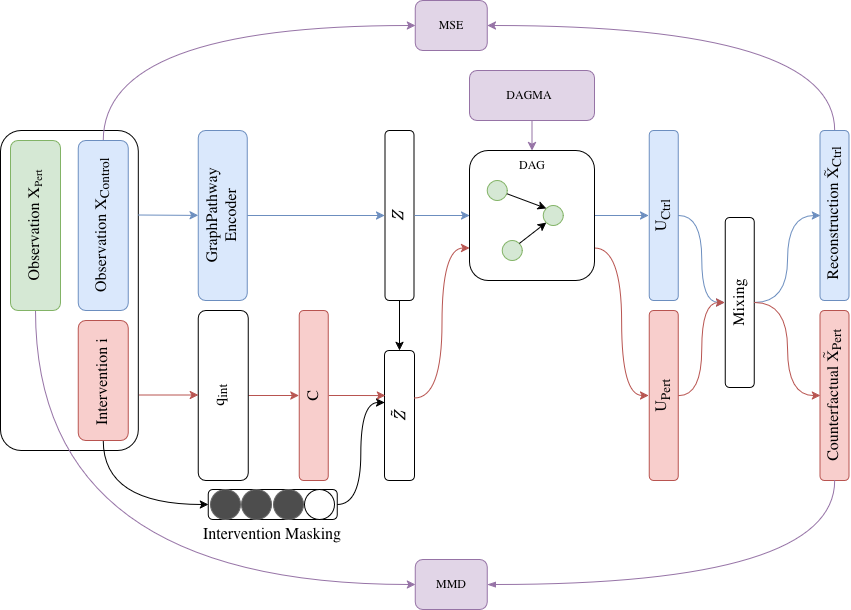
\includegraphics[width=.8\textwidth]{gfx/full_framework_modified.png}
    \caption{
        Detailed schematic of the \gls{raptorgraph} framework.
        The preconditioned GraphPathway Encoder enforces a sparse mapping from the high-dimensional gene expression space ($\sR^{\observeddim}$) to the learned meta-pathways ($\sR^{\latentdim}$).
        The DAGMA-based DAG operates on the latent representations to learn a directed acyclic graph ($\graph$) representing the causal relationships between the learned meta-pathways.
        The model is trained end-to-end using a composite loss function comprised of several terms: a reconstruction loss (\gls{mse}), a distributional loss (\gls{mmd}) on interventional predictions, a KL Divergence on the \gls{vae} latent variables, and an acyclicity constraint from the DAGMA layer.
    }
    \label{fig:app:architecture:overview}
\end{figure}

%-------------------------------------------------------------------------------
% Subsection: GraphPathway Encoder Architecture
%-------------------------------------------------------------------------------
% [ADDITION: Addressing Reviewer yvAn] Reinforcing the end-to-end/joint optimization nature 
% of the GraphPathway encoder and DAGMA module.
\revised{The entire framework is trained end-to-end. During optimization, gradients from the \glsentryshort{dagma} loss $\dagmaloss$ backpropagate through the GraphPathway encoder, ensuring that the latent representation is regularized to expose the underlying causal structure.}

%-------------------------------------------------------------------------------
\subsection{Joint Discovery via Causal Transform Layer}
\label{app:arch:causal_transform}
%-------------------------------------------------------------------------------

A common misunderstanding in causal representation learning is the perceived decoupling between representation learning (\glsentryshort{vae}) and causal structure learning (\glsentryshort{dag} discovery). In \glsentryshort{raptorgraph}, these components are architecturally integrated through a \textbf{Causal Transform} layer.

\paragraph{1. The Causal Layer in the Forward Pass}
The \glsentryshort{dag} module is not a post-hoc analysis tool; it is a differentiable layer situated between the encoder and the decoder. In the forward pass, the exogenous noise $\exonoise$ (output of the GraphPathway encoder) is transformed into endogenous pathway activities $\latentcausalvars$ by solving the structural equation:
\begin{equation}
    \latentcausalvars = \latentcausalvars \graphmatrix^T + \exonoise \implies \latentcausalvars = \exonoise(\identitymatrix - \graphmatrix)^{-T}
\end{equation}
where $\graphmatrix$ is the learnable adjacency matrix. This $\latentcausalvars$ is then passed to the decoder to produce the reconstruction $\predictedvariable$.

\paragraph{2. Joint Optimization by Reconstruction}
Because the \glsentryshort{dag} layer is part of the autoencoder's forward pass, the reconstruction loss $\mseloss = \|\variables - \predictedvariable\|^2$ backpropagates gradients through the decoder, the \glsentryshort{dag} layer ($\graphmatrix$), and the encoder. This ensures that the latent space and the causal graph are \textbf{jointly optimized} to satisfy the data-fit objective. 

%-------------------------------------------------------------------------------
\subsection{The Necessity of Hard Architectural Constraints vs. Soft Alignment}
\label{app:arch:hard_vs_soft}
%-------------------------------------------------------------------------------

We formally justify the use of hard architectural constraints (the GraphPathway encoder) over soft alignment mechanisms (e.g., concept bottleneck supervision).

\paragraph{1. Preventing Intervention Spillover}
Dense encoders (MLPs) suffer from intervention spillover, where a sparse perturbation in gene space propagates into a dense signal in latent space. While soft losses can encourage alignment, they do not provide the \textbf{guaranteed isolation} required for identifiable causal discovery. The hard GraphPathway constraint ensures that the interventional entry point is architecturally limited to a unique node ($\nabla_{do(x_i)} z_j = 0$ for $i \neq j$), eliminating the "winner-take-all" misattribution common in soft-aligned models.

\paragraph{2. Preserving Biological Interpretability for GI Scoring}
The identification of complex Genetic Interactions (e.g., Synergy, Redundancy) requires a strict 1-1 mapping between perturbation targets and causal factors. Soft alignment often leads to "leaky" representations where a single biological program is smeared across multiple latent variables. Our results demonstrate that the hard structural constraint is essential for maintaining the fidelity required to score these non-additive interactions accurately.

\subsection{GraphPathway Encoder Architecture}
\label{app:graphpathway}
%-------------------------------------------------------------------------------

The GraphPathway Encoder is a custom neural network layer designed to solve the Intervention Spillover Problem through a principled architectural design.
It combines a preconditioned weight matrix to deconfound known perturbation effects with a multi-subgraph structure to capture complex, non-linear gene interactions.

%-------------------------------------------------------------------------------
% Subsubsection: Deconfounding through Preconditioning
%-------------------------------------------------------------------------------
\subsubsection{Deconfounding through Preconditioning}
\label{app:graphpathway:preconditioning}
%-------------------------------------------------------------------------------

The foundational component of the encoder is its preconditioned weight matrix, which enforces the single-node intervention assumption required for causal identifiability.
As described in \cref{subsec:methods:graphpathway}, the layer's primary weight matrix $\weightmatrix$ is structured as a block matrix with a strictly diagonal top-left block.
This structure guarantees that each known perturbed gene has a direct, isolated influence on exactly one latent pathway, while the zero-block explicitly prevents its effect from spilling over into other pathways.
This design transforms the encoder into a deterministic modulator for known interventions, allowing the intervention mask $\maskvector$ to be fixed by the architecture rather than being a learned (and potentially dense) variable.
\revised{By explicitly blocking the spillover of the intervention effect into other pathways via the zero-block,} this design transforms the encoder into a deterministic modulator for known interventions, allowing the intervention mask $\maskvector$ to be fixed by the architecture rather than being a learned (and potentially \revised{confounded}) variable.

%-------------------------------------------------------------------------------
% Subsubsection: Modeling Non-Linear Interactions with Subgraphs
%-------------------------------------------------------------------------------
\subsubsection{Modeling Non-Linear Interactions with Subgraphs}
\label{app:graphpathway:subgraphs}
%-------------------------------------------------------------------------------

To move beyond a purely linear model and capture the complex, non-linear dynamics of biological processes, the architecture learns $\numgraphs$ distinct representations for each pathway.
This is achieved by first applying a masked linear layer that maps the input genes $\variables$ to an intermediate representation.
This layer's weight matrix is derived by repeating the base preconditioned mask $\numgraphs$ times, creating $\numgraphs$ parallel, similarly conditioned subgraphs that are initialized differently to learn diverse feature mappings.
The initial activation vector, $\pathwayactivation^{(g)}$, for each subgraph $g$ is computed as:
\begin{equation}
    \pathwayactivation^{(g)} = \activationfunc(\weightmatrix^{(1, g)}\variables + \vect{b}^{(1,g)}) \quad \text{for } g=1, \dots, \numgraphs
\end{equation}
where each layer-specific weight matrix $\weightmatrix^{(1, g)}$ has the same block-diagonal structure.

An intermediate \emph{Interaction Block} then processes these subgraph activations to model higher-order dependencies.
This block applies a series of pathway-specific linear transformations and non-linear activations to the set of $\numgraphs$ activations within each pathway, enabling the model to learn complex interactions between the different feature mappings before the final aggregation step.

Finally, the processed subgraph activations are aggregated into the final pathway representations using a grouped 1D convolution.
This operation has a kernel size of $\numgraphs$ and is configured with $\latentdim$ groups, making it equivalent to applying a separate, pathway-specific linear layer to the set of $\numgraphs$ subgraph activations for each pathway.
This learns an optimal linear combination of the non-linear subgraph features to produce the final parameters for the latent distributions, $\vect{\mu}_{\latentvars}$ and $\vect{\sigma}_{\latentvars}$.

%-------------------------------------------------------------------------------
% Subsubsection: Implementation Details of GraphPathway
%-------------------------------------------------------------------------------
\subsubsection{Implementation Details of GraphPathway}
\label{app:graphpathway:implementation}
%-------------------------------------------------------------------------------

The specific implementation used in our model is the `InteractingGraphPathwayLayer`.
This layer encapsulates the preconditioning, multi-subgraph mapping, and interaction blocks into a single module.
To model complex, non-linear biological processes, each pathway learns its own unique set of interaction weights within the interaction block.
This design provides greater expressive power, as it allows the model to capture distinct interaction dynamics for each biological process.
When configured for a variational autoencoder, the output channel dimension of the final grouped convolution is doubled, allowing the layer to directly produce both the mean $\vect{\mu}_{\latentvars}$ and variance $\vect{\sigma}_{\latentvars}$ for each latent pathway.

%-------------------------------------------------------------------------------
% Subsection: Deep Causal Graph Learning with DAGMA
%-------------------------------------------------------------------------------
\subsection{Deep Causal Graph Learning with DAGMA}
\label{app:dagma}
%-------------------------------------------------------------------------------

This subsection details the DAGMA framework for causal discovery, the rationale for its adaptation within our deep learning model, and the key implementation principles required for stable and effective graph learning in a \gls{vae} context.

%-------------------------------------------------------------------------------
% Subsubsection: Theoretical Background: From NOTEARS to DAGMA
%-------------------------------------------------------------------------------
\subsubsection{Theoretical Background: From NOTEARS to DAGMA}
\label{app:dagma:background}
%-------------------------------------------------------------------------------

A fundamental challenge in causal discovery is the combinatorial nature of learning a \gls{dag}, as the number of possible graphs grows super-exponentially with the number of variables.
A breakthrough was achieved by NOTEARS~\citep{zheng2018dags}, which reformulated this discrete problem into a continuous optimization problem amenable to gradient-based methods.
The core innovation was a differentiable function, $h(\graphmatrix)$, whose value is zero if and only if the weighted adjacency matrix $\graphmatrix$ represents a \gls{dag}.
The original NOTEARS constraint is based on the matrix exponential:
\begin{equation}
    h(\graphmatrix) = \tr(e^{\graphmatrix \circ \graphmatrix}) - \latentdim = 0
    \label{eq:app:notears_constraint}
\end{equation}
where $\tr(\cdot)$ is the trace of the matrix and $\graphmatrix \circ \graphmatrix$ is the element-wise (Hadamard) product.
This function cleverly sums all cycles of all possible lengths in the graph; it equals zero only if no cycles exist.

DAGMA~\citep{bello2022dagma} builds upon this continuous optimization framework but introduces a new, log-determinant-based acyclicity characterization that often leads to faster and more stable convergence.
The DAGMA acyclicity constraint is:
\begin{equation}
    h_s(\graphmatrix) = -\log\det(s\identitymatrix - \graphmatrix \circ \graphmatrix) + \latentdim\log s = 0
    \label{eq:app:dagma_constraint}
\end{equation}
where $s>0$ is a scaling scalar.
This function is based on the principle that a matrix corresponds to a \gls{dag} if and only if all eigenvalues of its squared adjacency matrix are zero.
The log-determinant acts as a barrier, approaching infinity as the graph's structure approaches a cycle, while being minimized at zero exclusively for \glspl{dag}.

%-------------------------------------------------------------------------------
% Subsubsection: The DAGMA Optimization Framework
%-------------------------------------------------------------------------------
\subsubsection{The DAGMA Optimization Framework}
\label{app:dagma:optimization}
%-------------------------------------------------------------------------------

The full optimization problem is to minimize a score function that measures how well the graph fits the data, subject to the acyclicity constraint.
For a linear model with latent variables $\latentvars$, the score function $\scorefunc(\graphmatrix)$ is typically the mean squared error of reconstruction:
\begin{equation}
    \scorefunc(\graphmatrix) = \frac{1}{2n} \lVert \latentvars - \latentvars\graphmatrix \rVert_F^2
    \label{eq:app:dagma_score}
\end{equation}
The original DAGMA paper proposes a path-following approach that solves a sequence of unconstrained optimization problems:
\begin{equation}
    \min_{\graphmatrix} (\mu \cdot \scorefunc(\graphmatrix) + h_s(\graphmatrix))
\end{equation}
where $\mu$ is a hyperparameter that is gradually decreased towards zero during training.
As $\mu \to 0$, the penalty on violating acyclicity becomes infinitely strong, forcing the final solution for $\graphmatrix$ to be a \gls{dag}.

%-------------------------------------------------------------------------------
% Subsubsection: Rationale for a Modified DAGMA in a Causal Representation Learning
%-------------------------------------------------------------------------------
\subsubsection{Rationale for a Modified DAGMA in a Causal Representation Learning}
\label{app:dagma:rationale}
%-------------------------------------------------------------------------------

Integrating DAGMA into a \gls{vae} for interventional \gls{crl} requires careful design to ensure the model learns a meaningful causal graph.
Our implementation is guided by two core principles.

\paragraph{Principle 1: Learning the Invariant Graph from Observational Data.}
A foundational assumption is that the causal graph $\graphmatrix$ represents an invariant, underlying mechanism of the system.
Therefore, the DAGMA loss, which encourages the learning of this structure, must be computed exclusively on the latent representations of observational data ($\zobs$).
This teaches the model the fundamental causal rules from the system's natural dynamics.
The interventional data and their latent representations ($\zint$) are used to compute a separate discrepancy loss (e.g., \gls{mmd}).
This second loss teaches the model the consequences of breaking the causal rules, evaluating how well the learned graph functions as a simulator for interventions.
Applying the graph loss to interventional latents would create a conflicting objective, as an intervention by definition breaks the natural mechanism the graph is supposed to represent.

\paragraph{Principle 2: Isolating Gradient Flow via Input Detachment.}
The most critical design principle for stability is isolating the gradient flow between the \gls{vae}'s encoder and the DAGMA layer.
This is achieved by detaching the latent variable tensor ($\zobs$) before it is used in the score calculation ($\scorefunc(\graphmatrix, \zobs\text{.detach()})$).
This design choice has two key benefits.
First, it mimics the original DAGMA algorithm, which operates on a fixed dataset.
Second, and more importantly, it creates a separation of concerns: the encoder learns to produce a rich representation, and the DAGMA layer learns the graph of that representation.
Without detaching, gradients from the DAGMA score would flow back to the encoder, encouraging it to learn a trivial, simplistic latent space that is easy to fit, thereby destroying the quality of the representation.

%-------------------------------------------------------------------------------
% Subsubsection: Implementation Detail of DAGMA
%-------------------------------------------------------------------------------
\subsubsection{Implementation Detail of DAGMA}
\label{app:dagma:stability}
%-------------------------------------------------------------------------------

Several practical considerations are crucial for the stable application of DAGMA in a deep learning context.

\paragraph{Weight Initialization and Invertibility.}
To ensure stability from the start of training, the weights of the adjacency matrix $\graphmatrix$ are initialized from a uniform distribution in the range $[-0.1, 0.1]$.
This provides the optimizer with small, non-zero weights as a starting point.
This initialization also makes it highly probable that the matrix $(\identitymatrix - \graphmatrix)$ is well-conditioned and invertible, which is critical for the forward pass of the linear DAGMA model.
The forward pass solves the structural equation $\latentvars = \latentvars\graphmatrix + \exonoise$ for $\latentvars$, which requires computing $\exonoise(\identitymatrix - \graphmatrix)^{-1}$.
To handle potential numerical instability, our implementation first attempts to solve the linear system directly.
If this fails due to a singular or ill-conditioned matrix, it robustly falls back to using the Moore-Penrose pseudo-inverse, guaranteeing a stable forward pass throughout training.

\paragraph{Input Normalization.}
A common failure mode is the collapse of the graph weights in $\graphmatrix$ to a trivial near-zero solution.
This is prevented by applying a normalization layer (e.g., `LayerNorm`) to the latent inputs ($\zobs$ and $\zint$) before they enter the DAGMA layer.
This ensures the score term has a consistent magnitude, providing a strong and stable gradient signal that encourages the model to learn a non-trivial graph.

\paragraph{Numerical Precision.}
The acyclicity constraint $h_s(\graphmatrix)$ is theoretically guaranteed to be non-negative.
However, due to floating-point limitations, it can sometimes become a very small negative number.
To handle this, the calculated value is clamped at zero, which respects the theoretical constraint while gracefully handling practical numerical artifacts.


\clearpage
%===============================================================================
\section{Training Configurations and Analysis Setup}
\label{app:training_configs}
%===============================================================================

\subsection{Model Architectures and Training Hyperparameters}
To establish a fair and reproducible benchmark, we standardized key architectural and training hyperparameters for all models, primarily based on the default configurations provided in their respective publications and source code. This approach ensures that performance differences can be attributed to the models' core methodologies rather than variations in setup. Table \ref{tab:model_architectures} details the specific architectural parameters, such as latent dimension size and the number of transformer layers, while Table \ref{tab:training_hyperparameters} outlines the training parameters used for each model, including optimizer, learning rate, and batch size. Notably, gradient clipping was employed exclusively for the scGPT model, as this is a standard and necessary technique to ensure numerical stability during the training of large transformer-based architectures.

\revised{For a complete list of hyperparameters and reproducibility instructions, please refer to the `configs/` directory in our code repository and the accompanying `README.md`.}

% Table S1
\begin{table}[ht]
\centering
\caption{Detailed Model Architectures}
\label{tab:model_architectures}
\begin{tabular}{lcccc}
\hline
\textbf{Hyperparameter} & \textbf{dVAE} & \textbf{SENA} & \textbf{scGPT} & \textbf{RAPTORGraph} \\
\hline
Latent Dimension ($z_{dim}$) & 105 & 105 & N/A & \revised{109} \\
Embedding Size ($embsize$) & N/A & N/A & 512 & \revised{N/A} \\
Transformer Layers ($nlayers$) & N/A & N/A & 12 & \revised{N/A} \\
Attention Heads ($nheads$) & N/A & N/A & 8 & \revised{N/A} \\
Feed-Forward Dimension ($d_{hid}$) & N/A & N/A & 512 & \revised{904} \\
Hidden Layers (Encoder) & 1 (128 units) & 1 (128 units) & N/A & \revised{N/A} \\
Activation Functions & LeakyReLU & LeakyReLU & GELU & \revised{SiLU} \\
\hline
\end{tabular}
\end{table}

% Table S2
\begin{table}[ht]
\centering
\caption{Detailed Training Hyperparameters}
\label{tab:training_hyperparameters}
\begin{tabular}{lcccc}
\hline
\textbf{Hyperparameter} & \textbf{dVAE} & \textbf{SENA} & \textbf{scGPT} & \textbf{RAPTORGraph} \\
\hline
Optimizer & Adam & Adam & AdamW & \revised{AdamW} \\
Learning Rate & $1\times10^{-3}$ & $1\times10^{-3}$ & $1\times10^{-4}$ & \revised{$1\times10^{-4}$} \\
Training Batch Size & 32 & 32 & 16 & \revised{256} \\
Evaluation Batch Size & 32 & 32 & 32 & \revised{256} \\
Epochs & 100 & 100 & 30 & \revised{100} \\
\hline
\end{tabular}
\end{table}


%-------------------------------------------------------------------------------
% III. EXPERIMENTAL METHODOLOGY
%-------------------------------------------------------------------------------
\clearpage
%===============================================================================
\section{Rationale For Global Pairing through Optimal Transport}
\label{app:ot}
%===============================================================================

As discussed in \cref{sec:methods}, random pairing of control and perturbed cells leads to mean collapse. Here, we detail the mechanism behind this phenomenon and the mathematical formulation of our \gls{ot} solution.

\subsection{Mechanism of Mean Collapse}

For a given interventional sample (e.g., cell $i$, in which gene $A$ was perturbed), a randomly selected observational sample (e.g., cell $j$) from the batch is highly unlikely to be an appropriate counterfactual. 
The biological state of cell $j$ may differ substantially from that of cell $i$ prior to the perturbation.
Consequently, the model must learn a transformation from an often noisy and biologically irrelevant initial state. 
Across thousands of training iterations, a single interventional sample is paired with hundreds of different random controls. Each pairing provides a distinct and noisy gradient signal. 
The optimiser seeks to minimise the loss on average across these inconsistent pairings and converges on a simple solution: predicting the mean of the target distribution. The random noise from the poor counterfactuals averages to zero, leaving only the central tendency as a stable learning signal. Ultimately, the objective function effectively becomes an expectation over these random pairings. The model learns that the most reliable strategy to achieve a low expected loss is to ignore the specifics of the randomly chosen input and produce an average output. The optimisation landscape is thereby smoothed in a manner that makes the `mean prediction' an attractive local minimum.

\begin{figure}[tb]
    \centering
    \begin{subfigure}{0.45\linewidth}
        \centering
        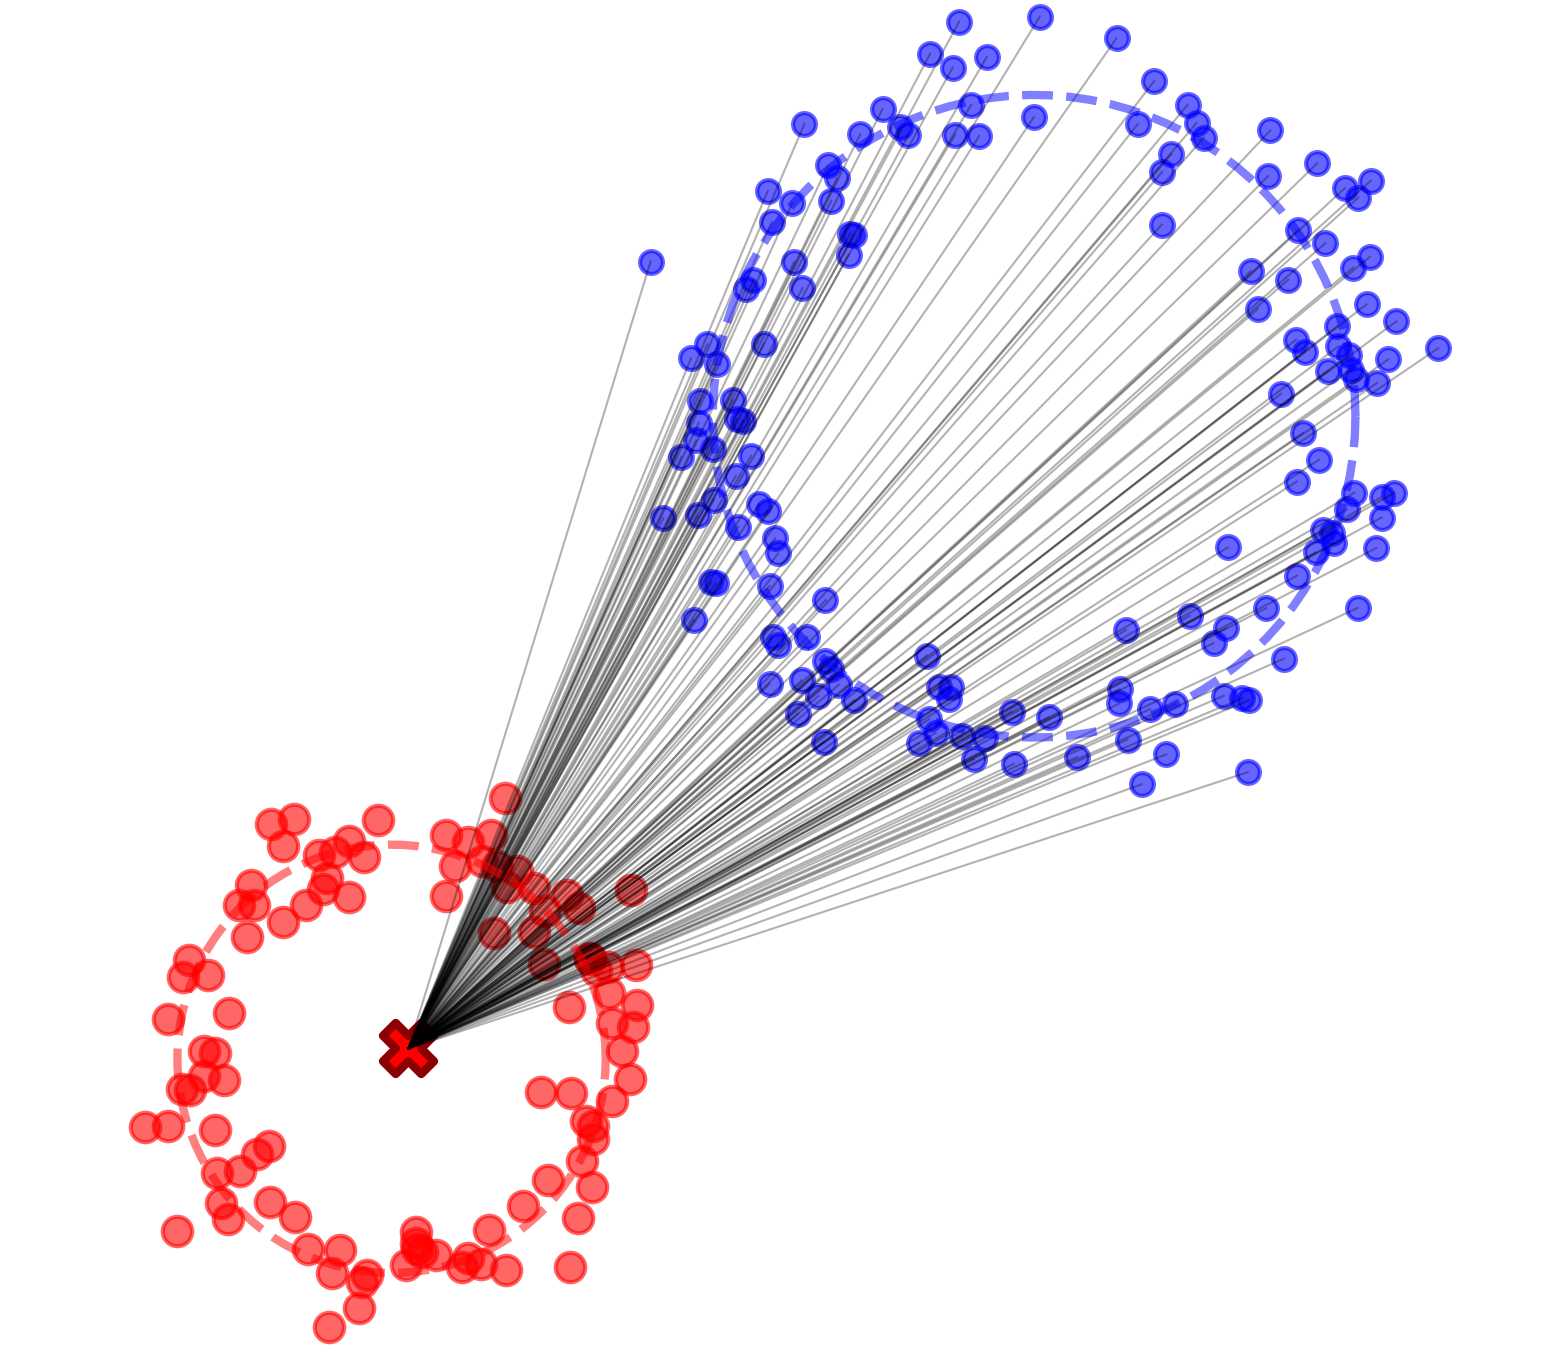
\includegraphics[width=\linewidth]{gfx/OT.png}
        \caption{Random pairing}
        \label{fig:app:ot_comparison_a}
    \end{subfigure}
    \hfill
    \begin{subfigure}{0.45\linewidth}
        \centering
        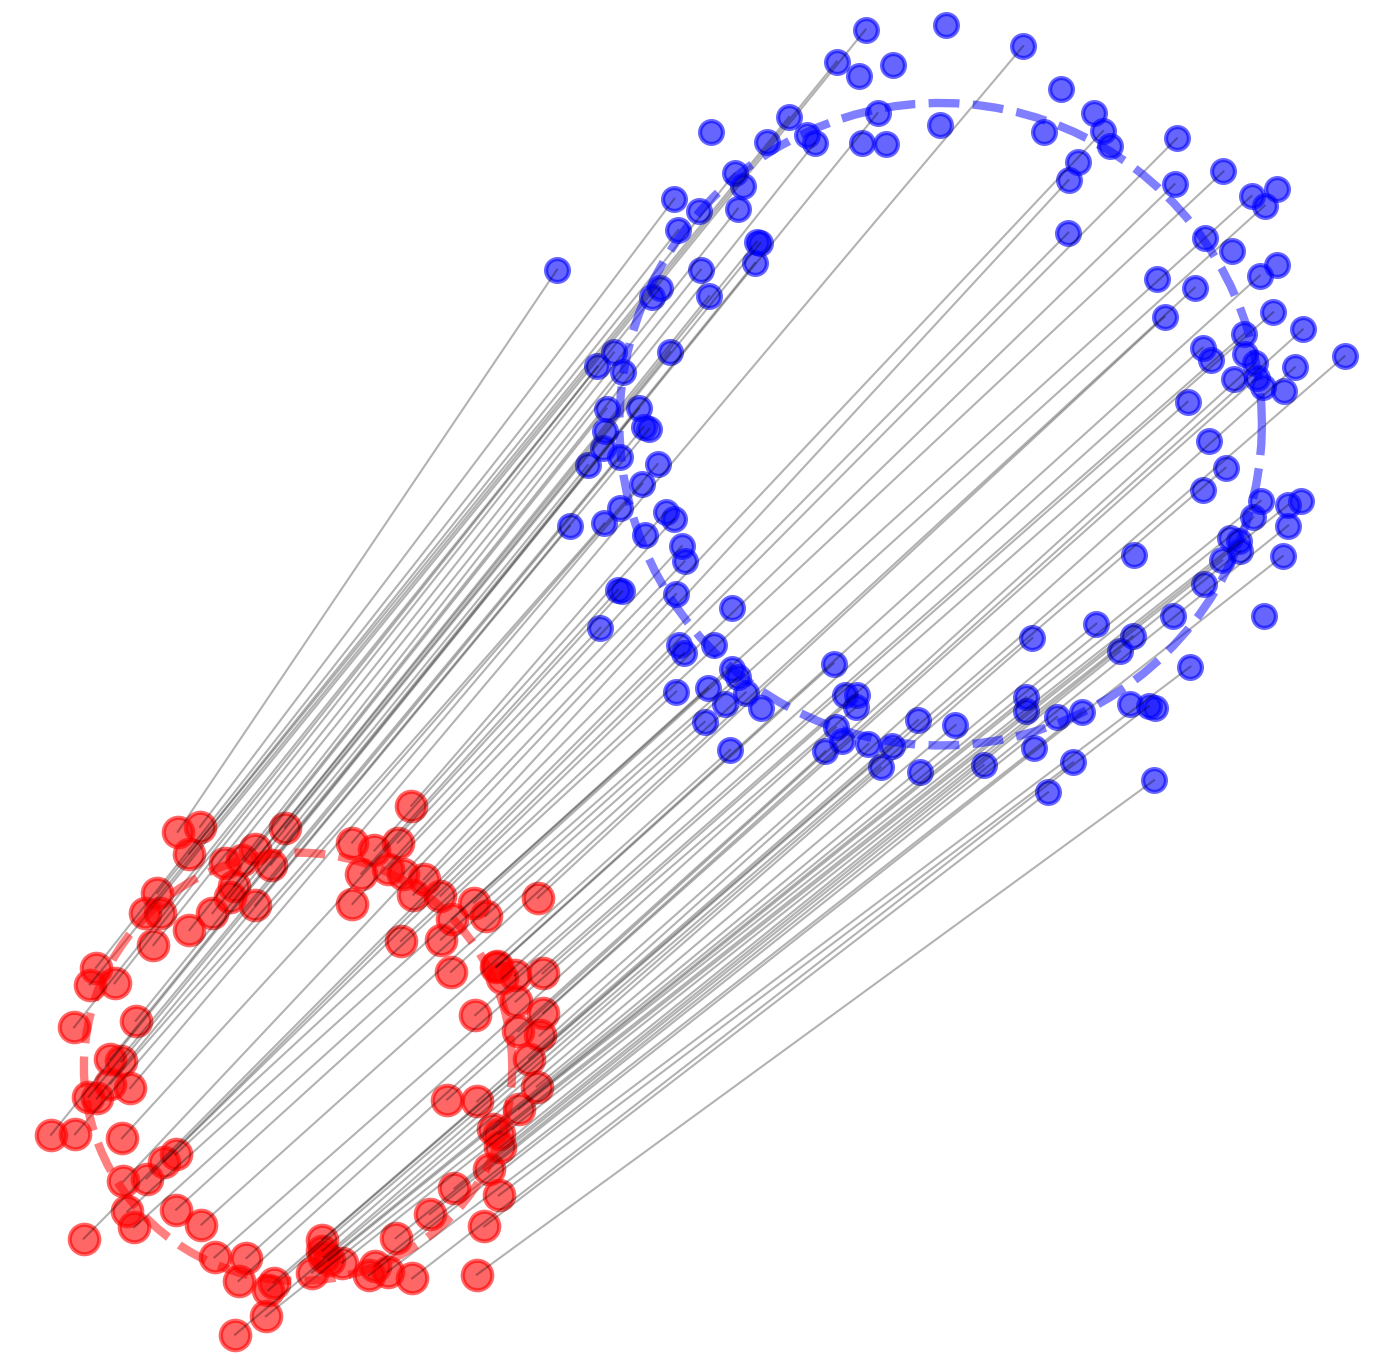
\includegraphics[width=\linewidth]{gfx/ot_comparison.png}
        \caption{Optimal Transport}
        \label{fig:app:ot_comparison_b}
    \end{subfigure}
    \caption{
        \textbf{Comparison of random pairing vs. Optimal Transport.}
        (a) Random pairing collapses the source distribution towards the target mean (mean collapse).
        (b) Optimal Transport pairing preserves the underlying population structure and biological heterogeneity.
    }
    \label{fig:app:ot_comparison}
\end{figure}

Rather than creating noisy one-to-one random pairs, \glsentryshort{ot} considers the entire population of observational and interventional latents. 
It computes an optimal flow of probability mass from the observational to the interventional distribution. This flow represents the most efficient method of morphing one entire point cloud into the other. The flow implicitly creates meaningful pairings.
Each interventional sample is matched with the observational sample(s) that are closest in gene expression space, providing the best possible counterfactuals within the given populations.
\revised{The theoretical properties of \glsentryshort{ot} ensure that it robustly preserves the inherent heterogeneous subpopulation structures by minimizing the ground movement cost, a feature critical for reliable counterfactual prediction.}

\subsection{Formal Derivation of Mean Collapse}
\revised{
We formally demonstrate why the random pairing strategy used in many current approaches fails to capture heterogeneous cellular responses.
Let $\variables \in \observsupport$ represent the control (source) cell and $\variables' \in \interventionaldist$ represent the perturbed (target) cell under intervention $p$. A generative model $\practicalencoder(\variables, p)$ aims to minimize the expected reconstruction error:
\begin{equation}
    \mseloss(\theta) = \mathbb{E}_{\variables \sim \observsupport, \variables' \sim \interventionaldist} \left[ \| \variables' - \practicalencoder(\variables, p) \|^2 \right]
\end{equation}

By the principles of Minimum Mean Squared Error (MMSE) estimation, the optimal function $f^*(\variables, p)$ that minimizes this loss is the conditional expectation:

\begin{equation}
    f^*(\variables, p) = \mathbb{E}[\variables' \mid \variables, P=p]
\end{equation}
In the case of \textbf{random pairing}, the target cell $\variables'$ is selected independently of the input cell $\variables$ (i.e., $\variables' \perp \variables \mid P=p$). This conditional independence allows us to simplify the expectation:
\begin{equation}
    f^*(\variables, p) = \mathbb{E}[\variables' \mid P=p] = \bar{\variables}_p
\end{equation}
where $\bar{\variables}_p = \int \variables' p(\variables' \mid P=p) d\variables'$ is the population mean vector for all cells undergoing perturbation $p$. 

\textbf{Conclusion:} Under random pairing, the model's optimal mathematical strategy is to completely ignore the specific initial state $\variables$ and predict a constant mean response for the entire population. This results in a Jacobian $\nabla_{\variables} f \to 0$, effectively erasing any discoverable \textit{cell-specific treatment effects}. By using \gls{ot} to enforce a deterministic coupling where $I(\variables, \variables') > 0$, \glsentryshort{raptorgraph} ensures that the model preserves the biological trajectory of individual cells.
}

\subsection{Mathematical Formulation of Optimal Transport}
Let $\mu_s = \sum_{i=1}^n \frac{1}{n} \delta_{\zobs^{(i)}}$ and $\nu_t = \sum_{j=1}^m \frac{1}{m} \delta_{\zint^{(j)}}$ be the empirical measures of the source (control) and target (perturbed) latent distributions.
The Optimal Transport problem seeks a transport plan $\gamma \in \mathbb{R}_{+}^{n \times m}$ that minimizes the total cost:
\begin{equation}
    \min_{\gamma \in \Pi(\mu_s, \nu_t)} \langle \gamma, \mathbf{C} \rangle_F
\end{equation}
where $\mathbf{C}_{ij} = \| \zobs^{(i)} - \zint^{(j)} \|^2_2$ is the squared Euclidean cost matrix, and $\Pi(\mu_s, \nu_t)$ is the set of joint probability measures with marginals $\mu_s$ and $\nu_t$.
The resulting optimal plan $\gamma^*$ provides a probabilistic coupling. To obtain a deterministic mapping for training, we use the barycentric projection map, ensuring each control cell is paired with its optimal counterfactual representation in the perturbed domain.

% [ADDITION: Addressing Reviewer yvAn] Added technical comparison between Hungarian matching 
% and Sinkhorn OT to justify why "soft" probabilistic coupling is more stable for scRNA-seq.
\subsection{\revised{Alternative Pairing Strategies}}
\label{app:ot:alternatives}

\revised{
To contextualize the performance of Sinkhorn \gls{ot}, we compare it against two common structured pairing alternatives:
\begin{itemize}
    \item \textbf{Nearest Neighbor (NN) Matching:} For each perturbed cell $\variables' \in \mathcal{Y}_p$, we select the control cell $\variables \in \mathcal{X}$ that minimizes the Euclidean distance $\|\variables - \variables'\|_2$. This is a greedy, many-to-one mapping strategy. While computationally efficient, it often fails to preserve the global distribution of the control population, leading to redundant pairings and loss of heterogeneity.
    \item \textbf{Hungarian Matching (Linear Sum Assignment):} This approach solves the bipartite matching problem to find a strict one-to-one bijection between control and perturbed sets by minimizing the total assignment cost $\sum_{i} \mathbf{C}_{i, \sigma(i)}$. We implement this using the Kuhn-Munkres algorithm. While globally optimal in a discrete sense, the hard assignment is highly sensitive to outliers and sampling noise in \gls{scRNAseq} data, leading to the instability observed in our results.
\end{itemize}
}

\clearpage
%===============================================================================
\section{Experimental Methodology: Data and Evaluation}
\label{app:methodology}
%===============================================================================

\subsection{Training and Test Data Partitioning}
\label{app:methodology:partitioning}

To create a robust benchmark for evaluating the generalization capabilities of each model, we partitioned the~\cite{norman2019exploring} dataset based on the type of perturbation. The training dataset was composed of the complete set of control cells (i.e., those with non-targeting guides) and the complete set of cells from all available \textbf{single-gene perturbation} conditions. This approach ensures that the models are trained on the fundamental effects of individual gene knockdowns. The test dataset, conversely, consisted exclusively of cells from all \textbf{double-gene perturbation} conditions. These combinatorial perturbations were entirely held out from the training process. This training/test split was designed to specifically assess each model's ability to perform out-of-distribution prediction, where the primary task is to predict the effects of unseen combinatorial perturbations based on the learned effects of their individual constituent perturbations.

\clearpage
%===============================================================================
% APPENDIX: EVALUATION METRICS AND LOSS FUNCTIONS
%===============================================================================
\section{Evaluation Metrics and Loss Functions}
\label{app:metrics}
%===============================================================================

In this section, we provide detailed definitions for the key metrics used to quantitatively assess model performance.
To ensure a comprehensive evaluation, we employed a suite of metrics targeting different aspects of model capability.
We used the \gls{mse} for evaluating the reconstruction of basal cell states, the \gls{mmd} for evaluating the accuracy of out-of-distribution predictions for perturbed states, and a set of non-additive interaction scores to assess the model's ability to capture complex biological phenomena.
The calculation of these metrics was standardized across all benchmarked tools.

%-------------------------------------------------------------------------------
% Subsection: Mean Squared Error (MSE)
%-------------------------------------------------------------------------------
\subsection{Mean Squared Error}
\label{app:metrics:mse}
%-------------------------------------------------------------------------------

The \gls{mse} was used to measure each model's ability to faithfully reconstruct the gene expression profile of control (unperturbed) cells, with a lower \gls{mse} indicating better performance.
To ensure an unbiased evaluation, the set of control cells was randomly split into two non-overlapping halves: an input set and a ground truth set.
The evaluation proceeded in a batch-wise manner, where a batch of cells from the input set was fed to the model to generate reconstructions.
The \gls{mse} was then calculated between these reconstructed cells and a corresponding batch from the ground truth set.
The final reported \gls{mse} is the mean of the scores from all batches.
For a single batch of $\numsamplesobs$ cells with $\numgenes$ genes, the \gls{mse} is calculated as:
\begin{equation}
    \mseloss = \frac{1}{\numsamplesobs \cdot \numgenes} \sum_{i=1}^{\numsamplesobs} \sum_{j=1}^{\numgenes} (\variables_{ij} - \predictedvariable_{ij})^2
    \label{eq:app:mse}
\end{equation}
where $\variables_{ij}$ is the expression level of the $j$\-th gene in the $i$\-th true control cell, and $\predictedvariable_{ij}$ is the expression level of the $j$\-th gene in the $i$\-th reconstructed control cell.

%-------------------------------------------------------------------------------
% Subsection: Maximum Mean Discrepancy (MMD)
%-------------------------------------------------------------------------------
\subsection{Maximum Mean Discrepancy}
\label{app:metrics:mmd}
%-------------------------------------------------------------------------------

The \gls{mmd}~\citep{gretton2012kernel} is a metric used to measure the distance between two probability distributions based on the distance between their mean embeddings in a \gls{rkhs}.
It was used to measure the dissimilarity between the distribution of model-predicted gene expression profiles and the distribution of true, experimentally observed profiles for a given perturbation.

\subsubsection{The Kernel Function}
\label{app:metrics:mmd:kernel}

The \gls{mmd} relies on a kernel function, $\kernel(\cdot, \cdot)$, which is a symmetric, positive definite function that computes a notion of similarity between two samples.
A common choice for the kernel, and the one used in our work, is the Gaussian \gls{grbf} kernel:
\begin{equation}
    \kernel(\variables, \vy) = \exp\left(-\frac{\|\variables - \vy\|^2}{2\mmdsigmaMMD^2}\right)
    \label{eq:app:kernel_rbf}
\end{equation}
where $\mmdsigmaMMD$ is the bandwidth hyperparameter.

%-------------------------------------------------------------------------------
\subsubsection{Formal Definitions of MMD}
\label{app:metrics:mmd:definitions}
%-------------------------------------------------------------------------------

The squared \gls{mmd} between the true data distribution $\pdata$ and the model's learned distribution $\pmodel$ is defined in its population form as:
\begin{align}
    \mmd^2(\pdata, \pmodel) &= \E_{\variables, \variables' \sim \pdata} \bigl[ \kernel(\variables, \variables') \bigr] \notag \\
    &\quad - 2 \E_{\variables \sim \pdata, \predictedvariable \sim \pmodel} \bigl[ \kernel(\variables, \predictedvariable) \bigr] \notag \\
    &\quad + \E_{\predictedvariable, \predictedvariable' \sim \pmodel} \bigl[ \kernel(\predictedvariable, \predictedvariable') \bigr]
    \label{eq:app:mmd_population}
\end{align}
In practice, we use batches of data and compute the unbiased empirical estimator.
Given a batch of $\numsamplesobs$ true samples $\{\variables_i\}_{i=1}^\numsamplesobs \sim \pdata$ from matrix $\datamatrix$ and a batch of $\numsamplespred$ predicted samples $\{\predictedvariable_j\}_{j=1}^\numsamplespred \sim \pmodel$ from matrix $\predicteddatamatrix$, the estimator is:
\begin{align}
    \mmd_u^2(\datamatrix, \predicteddatamatrix) &= \frac{1}{\numsamplesobs(\numsamplesobs-1)} \sum_{i \ne j}^{\numsamplesobs} \kernel(\variables_i, \variables_j) \notag \\
    &\quad + \frac{1}{\numsamplespred(\numsamplespred-1)} \sum_{i \ne j}^{\numsamplespred} \kernel(\predictedvariable_i, \predictedvariable_j) \notag \\
    &\quad - \frac{2}{\numsamplesobs\numsamplespred} \sum_{i=1}^{\numsamplesobs} \sum_{j=1}^{\numsamplespred} \kernel(\variables_i, \predictedvariable_j)
    \label{eq:app:mmd_empirical}
\end{align}

%-------------------------------------------------------------------------------
\subsubsection{Multi-Kernel Implementation}
\label{app:metrics:mmd:multi_kernel}
%-------------------------------------------------------------------------------

\gls{mmd}~\citep{ren2010multiple,zhu2017maximum} extends the standard \gls{mmd} by using a convex combination of $\numkernels$ different kernels~\citep{gretton2012kernel}.
The squared \gls{mmd} is defined as a weighted sum of individual squared \glspl{mmd}:
\begin{equation}
    \mkmmd^2(\pdata, \pmodel) = \sum_{l=1}^{\numkernels} \mkmmdweights_l \cdot \mmd^2_{\kernel_l}(\pdata, \pmodel)
    \label{eq:app:mkmmd}
\end{equation}
where $\mkmmdweights_l \ge 0$ are the weights assigned to each kernel.

\subsubsection{Rationale for Using MMD}
\label{app:metrics:mmd:rationale}

The choice of \gls{mmd} over \gls{mse} for evaluating interventional predictions is motivated by two key factors.
First, \gls{mmd} captures holistic distributional shifts, including changes in variance, skewness, and modality, whereas \gls{mse} is only sensitive to the mean.
This is critical for modeling the heterogeneous biological response to a perturbation.
Second, state-of-the-art \gls{crl} models for interventional data often do not produce one-to-one pairings between predicted and ground-truth samples, making \gls{mse} computation impossible.
\gls{mmd} is a two-sample test that compares two sets of samples directly, which aligns perfectly with this setting.

%-------------------------------------------------------------------------------
\subsubsection{Hyperparameter Selection for MMD}
\label{app:metrics:mmd:hyperparameters}
%-------------------------------------------------------------------------------

The performance of the \gls{mmd} test is highly sensitive to the kernel bandwidth, $\mmdsigmaMMD$.
To establish a fair and consistent benchmark across all models, it was necessary to standardize this parameter.
We noted that different models, such as Discrepancy\gls{vae} and SENA~\citep{de2025interpretable}, use different default values.
The implementations often define a $\text{fix\_sigma}$ parameter, which relates to the standard kernel variance by $\text{fix\_sigma} = 2\mmdsigmaMMD^2$.
To standardize, we aligned with the value used in SENA.
Our benchmark, therefore, uses a \gls{mmd} implementation with a base $\text{fix\_sigma}$ set to 200.0 for all evaluations, which corresponds to a variance $\mmdsigmaMMD^2$ of 100.0.
This approach generates a series of kernels with varying bandwidths derived from this base value, ensuring the metric's scale and sensitivity were consistent and robust.

%-------------------------------------------------------------------------------
% Subsection: Kullback-Leibler (KL) Divergence
%-------------------------------------------------------------------------------
\subsection{KL Divergence}
\label{app:metrics:kld}
%-------------------------------------------------------------------------------

The Kullback-Leibler (KL) divergence term is a standard component of the \gls{vae} framework used to regularize the learned latent space.
It measures the information lost when the learned posterior distribution, $q(\latentvars|\variables)$, is used to approximate a predefined prior distribution, $p(\latentvars)$.
In our model, we assume a standard multivariate normal prior, $p(\latentvars) = \normaldist(\vect{0}, \identitymatrix)$.
The KL divergence term, $\kldloss$, encourages the encoder to produce latent representations that are both smooth and well-structured, preventing the model from assigning each input sample to a single, isolated point in the latent space (a form of overfitting).
The term is calculated as:
\begin{equation}
    \kldloss = \kl{q(\latentvars|\variables)}{p(\latentvars)} = -\frac{1}{2} \sum_{j=1}^{\latentdim} \left( 1 + \log(\sigma_j^2) - \mu_j^2 - \sigma_j^2 \right)
    \label{eq:app:kld}
\end{equation}
where $\mu_j$ and $\sigma_j$ are the mean and standard deviation produced by the encoder for the $j$-th latent pathway.

%-------------------------------------------------------------------------------
\subsection{Causal Graph Loss}
\label{app:metrics:dagma}
%-------------------------------------------------------------------------------

The causal graph structure between learned meta-pathways is identified by optimizing the DAGMA-based objective function~\citep{bello2022dagma}.
The loss function, $\dagmaloss$, is computed on the latent representations of observational data to learn the invariant causal rules of the biological system.
The objective integrates three key components: a data-fit score that measures how well the graph explains the observed dependencies, an L1 penalty to encourage structural sparsity, and a differentiable acyclicity constraint to ensure the resulting graph is a \gls{dag}.
The full causal graph loss is defined as:
\begin{equation}
    \dagmaloss = \mu \left( \scorefunc(\graphmatrix; \datamatrix) + \lambda_1 \|\graphmatrix\|_1 \right) + \acyclicityfunc(\graphmatrix)
    \label{eq:app:dagma_loss_full}
\end{equation}
where $\scorefunc(\graphmatrix; \datamatrix)$ is the data-fit score (typically the \gls{mse} of linear structural assignments in the latent space), $\|\graphmatrix\|_1$ is the L1 norm of the adjacency matrix $\graphmatrix$ controlled by sparsity hyperparameter $\lambda_1$, and $\acyclicityfunc(\graphmatrix)$ is the log-determinant acyclicity penalty.
The hyperparameter $\mu$ controls the trade-off between the data-fit score and the acyclicity constraint, following a path-following schedule during training as detailed in \cref{app:dagma:optimization}.

%===============================================================================
% \subsection{\revised{Benchmarking on Replogle2020 Dataset}}
% \label{app:metrics:replogle_benchmark}
%===============================================================================

% \revised{First, we measured the \gls{mse} between the ground truth and predicted profiles of control cells to evaluate how well each model reconstructs the basal, unperturbed cellular state.
% Second, we calculated the \gls{mmd} between the distributions of ground truth and predicted profiles for double-gene perturbations to assess the model's ability to capture the global transcriptional shift following a complex intervention.}

% \begin{table}[H]
% \color{blue} 
%     \centering
%     \begin{tabular}{lcc}
%         \toprule
%         {Metric} & {scGPT} & RAPTORGraph (ours) \\
%         \midrule
%         \gls{mmd} & 0.138 $\pm$ 0.000 & \textbf{0.137 $\pm$ 0.000} \\
%         \gls{mse} & 0.069 $\pm$ 0.000 & \textbf{0.054 $\pm$ 0.000} \\
%         \bottomrule
%     \end{tabular}
%     \caption{\revised{Results using the Replogle2020 dataset are averaged over $3$ runs. Values are mean $\pm$ variance.}}
%     \label{tab:objective_results_replogle}
% \end{table}

% \revised{To validate the generalization capabilities of \glsentryshort{raptorgraph} across different experimental contexts and cell lines, we extended our evaluation to include the large-scale single-cell CRISPR screen dataset from \citet{replogle_combinatorial_2020} as shown in \Cref{tab:objective_results_replogle}.
% As discussed in \cref{sec:results}, our primary comparative analysis prioritized the \citet{norman2019exploring} dataset due to the rigid architectural dependency of several baseline models (specifically SENA and Discrepancy VAE) on auxiliary files and preprocessing pipelines unique to that study.
% Adapting these confirmatory models to the distinct structure of the Replogle2020 dataset proved non-trivial.
% Additionally, we excluded the \glsentryshort{gears} model because it behaves in a fundamentally different way that is incompatible with our evaluation framework, making a fair and direct comparison impossible.
% Consequently, this supplementary benchmark is restricted to a direct comparison between \glsentryshort{raptorgraph} and \glsentryshort{scgpt}, demonstrating our model's robust performance and superior reconstruction fidelity on independent biological data.}

%===============================================================================
\subsection{Non-Additive Genetic Interaction Analysis}
\label{app:metrics:genetic_interaction}
%===============================================================================

To evaluate the models' ability to predict non-additive effects, we designed a genetic interaction analysis inspired by the Precision@10 metric introduced in the GEARS paper~\citep{roohani2024predicting}.
While the original study used a robust regression model, we opted for a more direct naive additive baseline, defined as the vector sum of single-perturbation effects over control ($\effectvector_A + \effectvector_B$).
We calculated five interaction scores by comparing the predicted double-perturbation effect ($\effectvector_{AB}$) to this baseline.
This unified metric was applied to all models to ensure a fair comparison.

The analysis follows a multi-step process for each double-gene perturbation.
First, ``effect vectors'' ($\effectvector$) are calculated for single and double perturbations by subtracting the mean gene expression profile of control cells from the mean profile of perturbed cells.
This is done for both ground truth data and model predictions.
The naive additive baseline assumes the double perturbation effect is a linear sum of individual effects:
\begin{equation}
    \effectvectornaive = \effectvector A + \effectvector B
    \label{eq:app:naive_additive}
\end{equation}
By comparing the true or predicted $\effectvector(A+B)$ to the individual and naive additive vectors, we compute raw scores for five distinct genetic interaction subtypes.
\begin{itemize}
    \item \emph{Synergy} and \emph{Suppression} are measured using a ratio of magnitudes:
    \begin{equation}
        \synergyscore = \frac{\ltwonorm{\effectvector(A+B)}}{\ltwonorm{\effectvectornaive}}
        \label{eq:app:synergy_ratio}
    \end{equation}

    \item \emph{Neomorphism} measures changes in the direction of the effect:
    \begin{equation}
        \neomorphismscore = 1 - \cossim{\effectvector(A+B)}{\effectvectornaive}
        \label{eq:app:neomorphism}
    \end{equation}

    \item \emph{Redundancy} measures functional overlap:
    \begin{equation}
        \redundancyscore = \min \big( \cossim{\effectvector(A+B)}{\effectvector A}, \cossim{\effectvector(A+B)}{\effectvector B} \big)
        \label{eq:app:redundancy}
    \end{equation}

    \item \emph{Epistasis} measures dominance:
    \begin{equation}
        \epistasiscore = \big\lvert \cossim{\effectvector(A+B)}{\effectvector A} - \cossim{\effectvector(A+B)}{\effectvector B} \big\rvert
        \label{eq:app:epistasis}
    \end{equation}
\end{itemize}
Final performance is measured using Precision@10.
For each interaction type, perturbations are ranked by their predicted score, and the top 10 are selected.
These are compared against a ground truth set of interactors, defined as those whose true score falls in the top 25\% (or bottom 25\% for suppression) for that category.
The Precision@10 score is the fraction of correct predictions in the top 10.

%===============================================================================
\subsection{Reverse Perturbation Analysis}
\label{app:metrics:reverse_perturbation}
%===============================================================================

To assess the models' understanding of genotype-phenotype relationships, we implemented an in silico reverse perturbation prediction task, inspired by the analysis in the scGPT study~\citep{cui2024scgpt}.
This task challenges a model to infer the causal genetic perturbation that induced a given transcriptomic state.

The analysis is conducted on a specific subset of 20 genes from the \citet{norman2019exploring} dataset, creating a controlled combinatorial search space.
For each unique perturbation condition $p$, we establish a ground truth mean expression profile, $\meanexpression_p$, by averaging the expression vectors of all cells for that condition:
\begin{equation}
    \meanexpression_p = \frac{1}{\numcells_p} \sum_{i=1}^{\numcells_p} \variables_{p,i}
    \label{eq:app:mean_expression}
\end{equation}
where $\numcells_p$ is the number of cells under perturbation $p$, and $\variables_{p,i} \in \realnumbers^\numgenes$ is the expression profile of the $i$-th cell.
The central component is the creation of a comprehensive in silico prediction database restricted to the 20-gene subset.
For each model, we generate a predicted expression profile $\predictedvariable_{A+B}$ for every unique combination of two genes, A and B.
This is achieved by feeding the model the ground truth mean control profile, $\meanexpression_{\text{ctrl}}$, and conditioning it on the desired double perturbation.
The prediction function $\predictionfunc$ for a given model is expressed as:
\begin{equation}
    \predictedvariable_{A+B} = \predictionfunc(\meanexpression_{\text{ctrl}}, \text{pert}=A+B)
    \label{eq:app:prediction_function}
\end{equation}
This results in a key-value database where each key is a double-perturbation identifier from the 20-gene subset, and the value is the corresponding predicted mean expression vector in $\realnumbers^\numgenes$.

With the prediction database established, we query it using the ground truth mean expression profiles of the experimentally observed double perturbations from the 20-gene subset.
For each true double perturbation $p_{true}$ present in the test set, its ground truth mean profile $\meanexpression_{p_{\text{true}}}$ is used as a query vector.
We then calculate the Euclidean distance between this query vector and every predicted vector $\predictedvariable_{p_{\text{pred}}}$ in the database:
\begin{equation}
    d(\mathbf{\meanexpression}_{p_{\text{true}}}, \mathbf{\predictedvariable}_{p_{\text{pred}}}) = \sqrt{\sum_{j=1}^{\numgenes} (\meanexpression_{p_{\text{true},j}} - \predictedvariable_{p_{\text{pred},j}})^2}
    \label{eq:app:euclidean_distance}
\end{equation}

The perturbations in the database are subsequently ranked based on their proximity to the query vector, from the smallest to the largest Euclidean distance.
This yields a ranked list of predicted perturbations that are most likely to have caused the observed cellular state.

To evaluate the ranking performance, we employ the ``Hit Rate @ K'' metric, which measures the frequency of successful retrievals within the top K predictions.
We define two variants of this metric to capture different aspects of prediction accuracy.

\emph{Correct Hit Rate @ K}: This is a stringent metric that measures the proportion of queries where the exact true perturbation is correctly identified within the top K ranked predictions.
It is formally defined as:
\begin{equation}
    \text{Correct Hit Rate @ K} = \frac{1}{|\mathcal{Q}|} \sum_{q \in \mathcal{Q}} \mathbb{I}(\text{rank}(p_q) \le K)
    \label{eq:app:correct_hitrate}
\end{equation}
where $\mathcal{Q}$ is the set of all query perturbations, $p_q$ is the true perturbation corresponding to query $q$, and $\mathbb{I}$ is the indicator function, which is 1 if the condition is met and 0 otherwise.

\emph{Relevant Hit Rate @ K}: This is a more lenient metric that assesses whether the model can identify at least one of the correct genetic components of a combinatorial perturbation.
A prediction is considered "relevant" if its set of perturbed genes has a non-empty intersection with the set of genes in the true perturbation.
The metric is defined as:
\begin{equation}
    \text{Relevant Hit Rate @ K} = \frac{1}{|\mathcal{Q}|} \sum_{q \in \mathcal{Q}} \mathbb{I}(\exists \hat{p} \in \text{TopK}(q) \text{ s.t. } \text{genes}(\hat{p}) \cap \text{genes}(p_q) \neq \emptyset)
    \label{eq:app:relevant_hitrate}
\end{equation}
where $\text{TopK}(q)$ is the set of top K predicted perturbations for query $q$, and $\text{genes}(p)$ is the set of constituent genes in perturbation $p$.
This metric rewards models that can correctly identify influential genes, even if the exact combination is not perfectly predicted.
Together, these two metrics provide a comprehensive evaluation of each model's ability to reverse-engineer the mapping from cellular phenotype back to genetic cause.

%===============================================================================
\subsection{Gene Set Enrichment Analysis}
\label{app:metrics:gsea_setup}
%===============================================================================

\revised{To validate the semantic meaning of the learned Directed Acyclic Graph, we performed a systematic Gene Set Enrichment Analysis.
We employed an in-silico perturbation strategy to define the biological identity of each latent variable:}
\begin{enumerate}
    \item \revised{Latent Perturbation: For each causal latent factor $\latentvars_i$ associated with a known gene perturbation, we artificially activated the factor in the latent space by setting the condition vector $\conditionvector$ such that the target component $\conditionvector_i=1$ and all other components $\conditionvector_{j \neq i}=0$.}
    \item \revised{Counterfactual Decoding: We decoded this perturbed latent state back to the gene expression space $\realnumbers^n$ to generate a batch of ``counterfactual'' expression profiles.}
    \item \revised{Differential Analysis: We computed the mean differential expression vector $\delta = \bar{x}_{int} - \bar{x}_{ctrl}$ relative to the control baseline.}
    \item \revised{Enrichment: This vector was used to create a ranked gene list, which was analyzed using the \texttt{gseapy} framework against the MSigDB Hallmark 2020 gene set collection.}
\end{enumerate}

\revised{This process allows us to independently verify if the latent factor $\latentvars_i$ actually encodes the biological function of its assigned gene $g_i$, assigning a verifiable ``biological label'' to the nodes of our learned graph.}
%===============================================================================
\subsection{Rationale for the Exclusion of GEARS from the Benchmark}
\label{app:metrics:gears_exclusion}
%===============================================================================

In designing this benchmark, our goal was to establish a fair and methodologically consistent framework for comparing models that predict the full distribution of single-cell gene expression profiles following perturbation.
While we considered including other prominent models such as GEARS, we ultimately excluded it from the final comparison due to fundamental incompatibilities between its predictive paradigm and our standardized evaluation framework.
The two primary reasons for its exclusion are its prediction of a single population-average vector rather than a cell distribution, which is incompatible with our \gls{mmd} metric, and its non-equivalent handling of the control state, where it uses the precomputed mean of true control cells as a baseline rather than learning to reconstruct them.
Given these significant differences, we concluded that a fair and direct comparison between GEARS and the other models within our established framework was not possible.

% %===============================================================================
% \subsection{Rationale for the Use of a Single Dataset}
% \label{app:metrics:single_dataset}
% %===============================================================================

% For our comparative analysis, we exclusively utilized the single-cell perturbation dataset from \citet{norman2019exploring}.
% This decision was primarily driven by the need to ensure a fair and direct comparison across all evaluated models.
% Several of the baseline methods, notably SENA and dVAE, have published implementations with specific dependencies on auxiliary files and pre-processed data structures that are tailored to the Norman et al. dataset.
% Adapting these models to alternative datasets would have necessitated significant modifications to their data loading and processing pipelines.
% Such alterations could introduce confounding variables and potentially bias the evaluation, as the performance of these models might be sensitive to the specific data format and auxiliary information provided.

%-------------------------------------------------------------------------------
% IV. RESULTS AND VALIDATION
%-------------------------------------------------------------------------------
\clearpage
%===============================================================================
% APPENDIX: EXTENDED RESULTS
%===============================================================================

%===============================================================================
\section{Extended Results}
\label{app:extended_results}
%===============================================================================

%===============================================================================
\subsection{Extended Results: Reverse Perturbation Analysis}
\label{app:extended_results:reverse_perturbation}
%===============================================================================
\begin{figure}[ht]
    \centering
    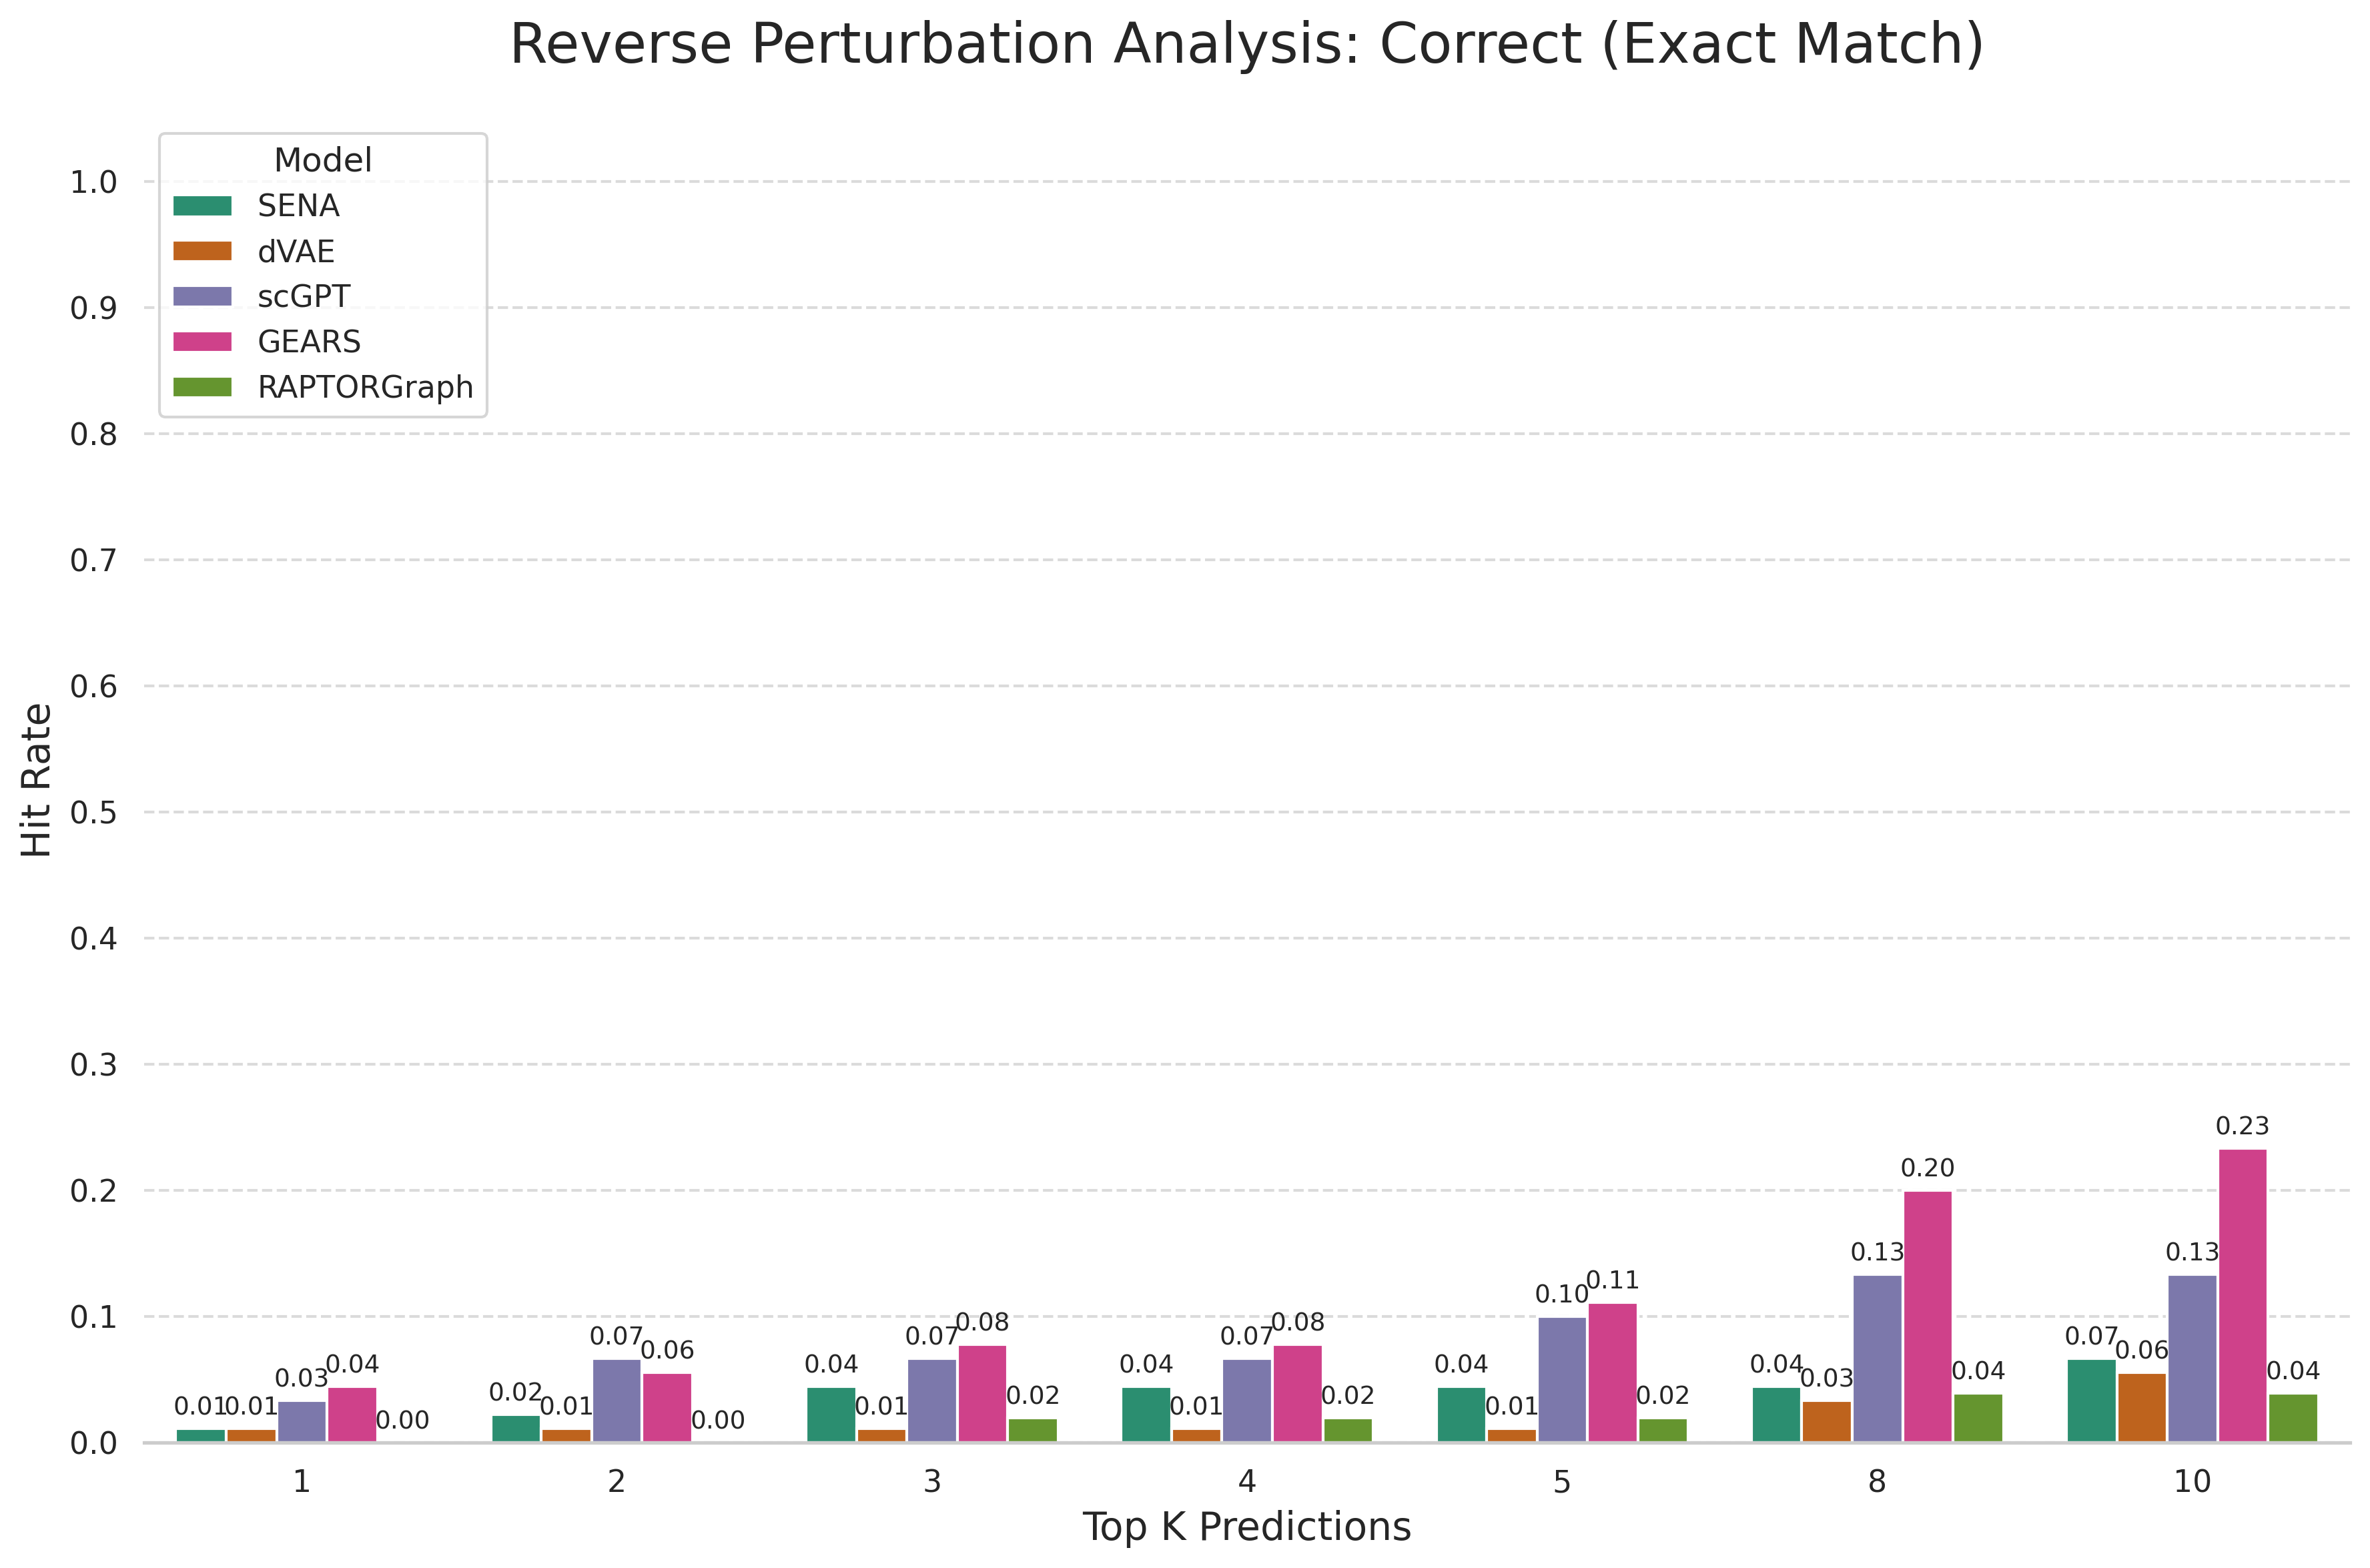
\includegraphics[width=0.75\linewidth]{gfx//results/hit_rate_at_k_correct_exact_match.png}
    \caption{Hit Rate @ K (correct) for the reverse perturbation task.
    The metric queries where the exact true perturbation is correctly identified within the top K ranked predictions.
    Results are averaged over 3 runs.}
    \label{fig:app:hit_rate_exact}
\end{figure}

\newpage

%===============================================================================
\subsection{\revised{Extended Results: Biological Validation of Learned \cmps{}}}
\label{app:extended_results:biological_validation}
%===============================================================================

\begin{figure}[ht]
    \centering
    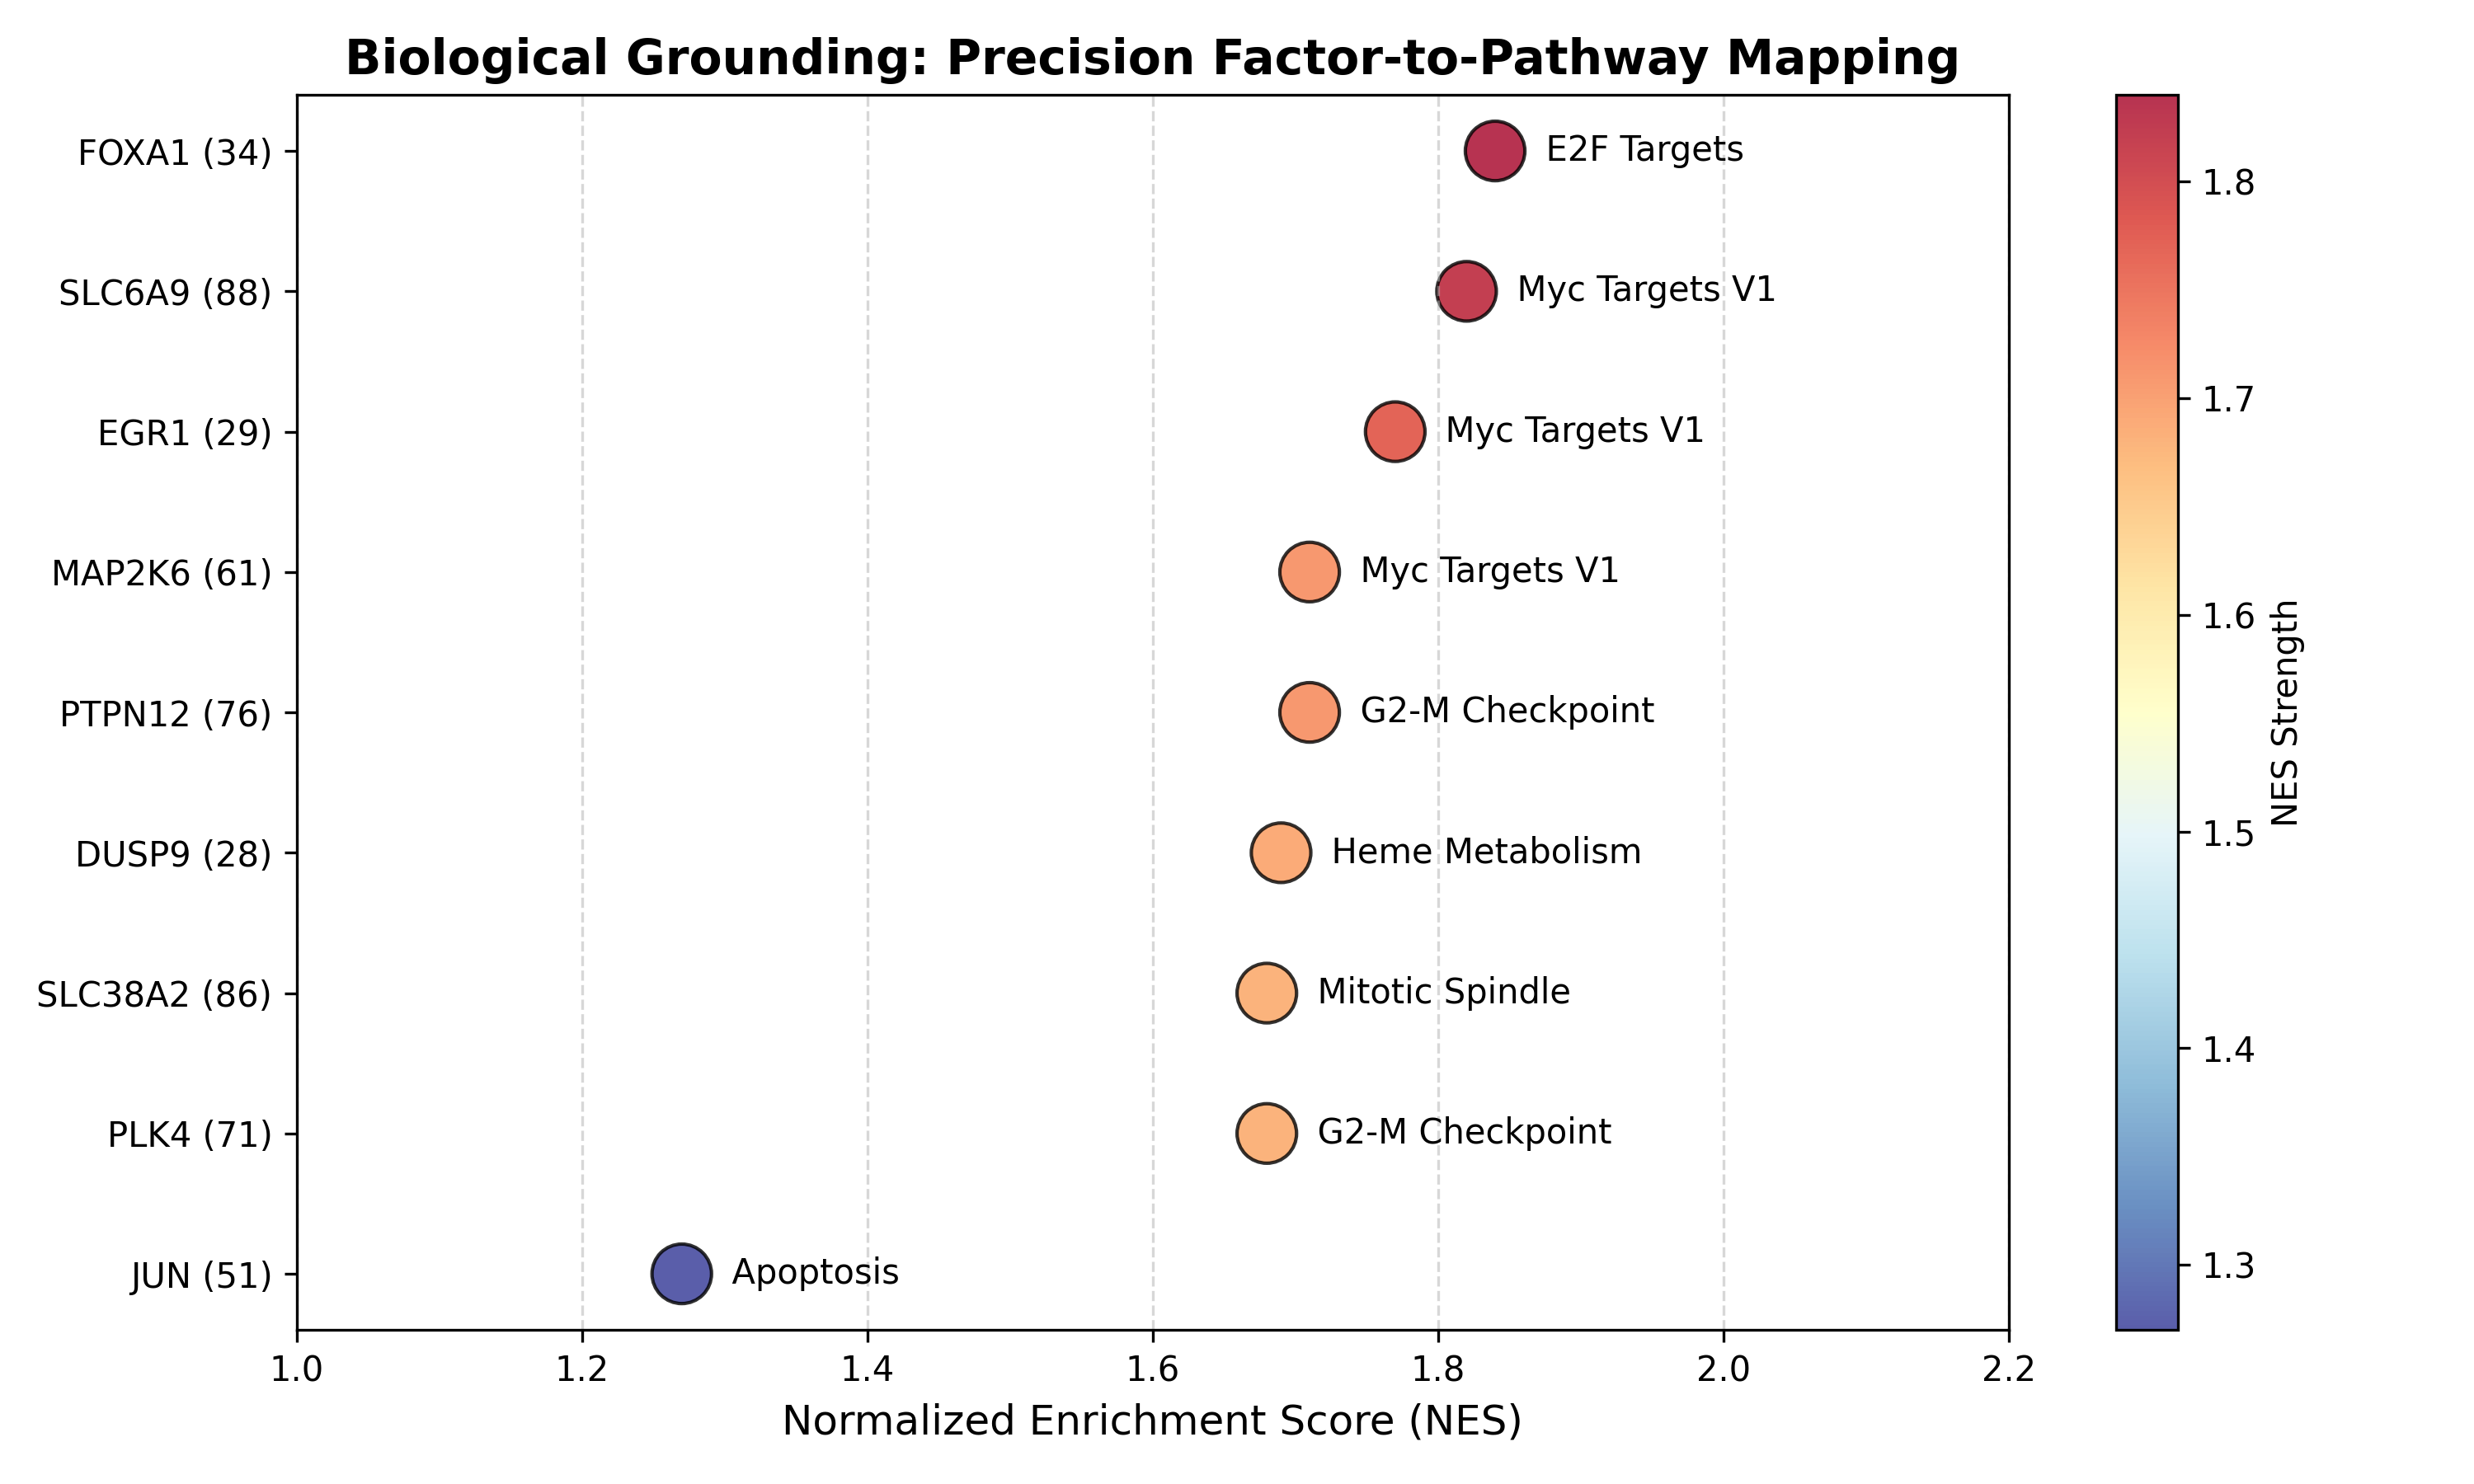
\includegraphics[width=0.8\textwidth]{gfx/rebuttal/fig_gsea_dots.png}
    \caption{\revised{\textbf{Biological Grounding (GSEA Dot Plot).} Visualization of Normalized Enrichment Scores (NES) for top-ranked causal factors, confirming precise mapping to established Hallmark pathways.}}
    \label{fig:rebuttal:gsea_dots}
\end{figure}

\begin{figure}[ht]
    \centering
    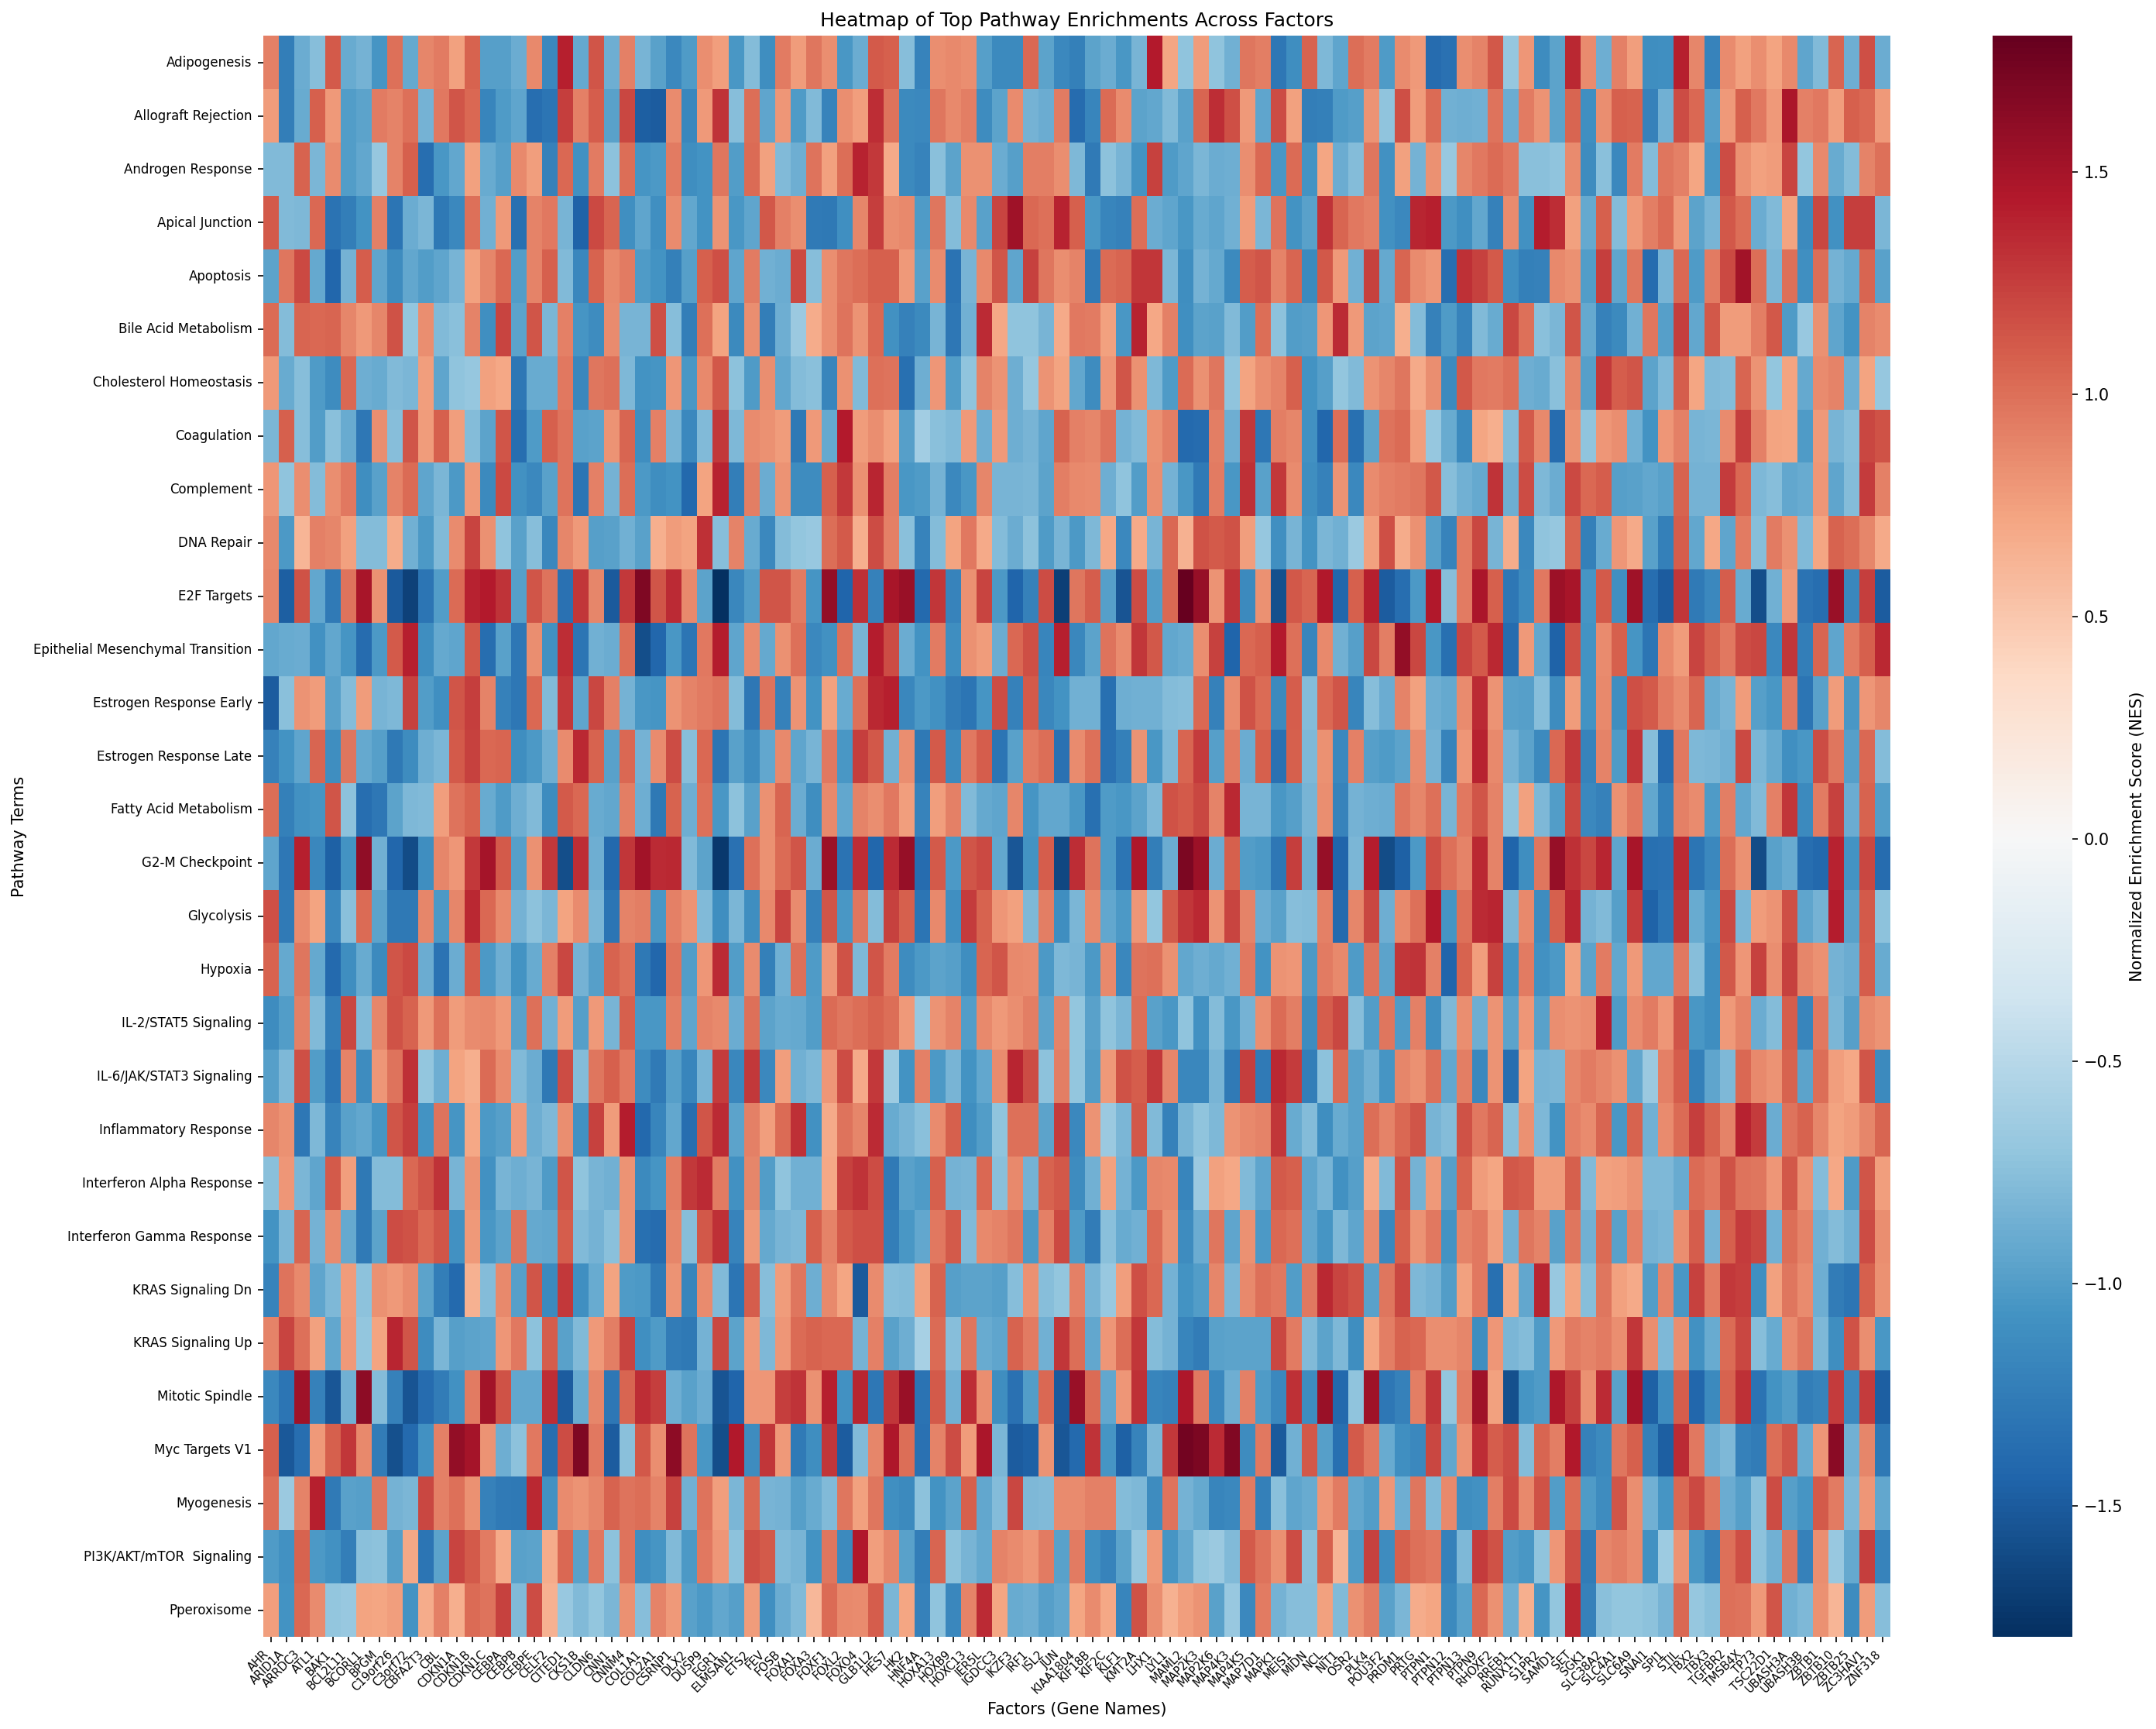
\includegraphics[width=\textwidth]{gfx/results/pathway_enrichment_heatmap.png}
    \caption{\revised{Heatmap of Top Pathway Enrichments Across Learned \cmps{}. 
    Each column corresponds to a specific \cmp{} ($z_i$) in the \gls{raptorgraph} model. Importantly, these labels are not post-hoc assignments; due to the GraphPathway encoder's preconditioning, each \cmp{} $z_i$ is architecturally constrained to mediate the effect of a specific gene perturbation (labeled on the x-axis).
    The rows represent biological pathways from the MSigDB Hallmark collection. The color intensity indicates the Normalized Enrichment Score (NES) derived from in-silico perturbation of that factor. The strong concordance between the architectural label and the biological result confirms that the model has successfully encoded the specific biological function of each gene into its corresponding \cmp{}.}}
    \label{fig:app:pathway_heatmap_supp}
\end{figure}

\revised{The GSEA analysis reveals that \gls{raptorgraph} captures distinct and biologically accurate programs. \Cref{fig:app:pathway_heatmap_supp} and \Cref{fig:rebuttal:gsea_dots} visualize the Normalized Enrichment Scores (NES) for the top enriched pathways across the learned factors. We highlight distinct biological programs captured by the model, verified against the known functions of their corresponding gene perturbations:}
\begin{enumerate}
    \item \revised{\textbf{Differentiation-Induced Arrest:} The \cmp{} linked to \textit{EGR1} displays massive negative enrichment for ``E2F Targets'' (NES $-1.79$, FDR $\approx 0.0$) and ``G2-M Checkpoint'' (NES $-1.72$, FDR $\approx 0.0$).
    EGR1 is a known tumor suppressor in K562 leukemia cells that drives differentiation along the megakaryocytic lineage, a process that necessitates a complete exit from the cell cycle \citep{ma_emodin_2019}.
    \gls{raptorgraph} correctly identifies this potent anti-proliferative program.}
    \item \revised{\textbf{Stress-Induced Growth Arrest:} The \cmp{} linked to the AP-1 subunit \textit{JUN} shows strong negative enrichment for ``E2F Targets'' (NES $-1.69$, FDR $< 0.001$) and ``G2-M Checkpoint'' (NES $-1.63$, FDR $< 0.002$). While often associated with inflammation, c-Jun is a central stress-response mediator; in the context of K562 cells, its activation drives a termination of cell division required for stress adaptation or differentiation \citep{shaulian_ap-1_2002, shaulian_mammalian_2000}.}
    \item \revised{\textbf{p53-Like Tumor Suppression:} The \cmp{} associated with \textit{TP73} displays significant negative enrichment for ``G2-M Checkpoint'' (NES $-1.60$, FDR $< 0.03$).
    \textit{TP73} is a functional homolog of \textit{TP53} (p53); its activation triggers downstream checkpoint signaling that arrests the cell cycle to prevent genomic instability \citep{kaghad_monoallelically_1997}.}
\end{enumerate}

\revised{
These findings confirm that the nodes in our learned DAG represent specific, identifiable biological mechanisms.
Consequently, the edges learned by the DAGMA module can be interpreted as causal regulatory links between these verified biological processes.
A detailed description of the methodology is provided in \cref{app:metrics:gsea_setup}.
}

%===============================================================================
\subsection{\revised{Extended Results: Computational Complexity of Optimal Transport Preprocessing}}
\label{app:extended_results:ot_complexity}
%===============================================================================

\revised{
    % \paragraph{Theoretical Complexity and Mitigation}
    We evaluated the computational cost of the proposed \gls{ot} pairing strategy compared to a random baseline. While random pairing scales linearly ($O(N)$), the \gls{ot} approach involves solving the \gls{emd} problem, which typically exhibits a worst-case complexity of $O(N^3 \log N)$. 
}

\revised{
    To mitigate this, the \gls{ot} pairing problem is formulated by taking the entire control population ($N_{ctrl} = 8,907$) and pairing it independently with each specific intervened population (i.e., cells sharing the same perturbation label, $N_k$ in the hundreds). 
    This effectively segments the total perturbed dataset ($N = 108,497$) into many smaller, manageable \gls{ot} problems, significantly reducing the $N$ in the $O(N^3 \log N)$ complexity for each individual transport plan and enabling efficient parallelization.
}

\revised{
    % \paragraph{Empirical Performance Benchmarks}
    We quantified the overhead of \gls{ot} preprocessing on a workstation equipped with an Intel Core i9-9900K CPU (8 cores, 16 threads) and 64 GB RAM.
    The \gls{ot} preprocessing added approximately 34 seconds to the baseline execution time (Random: 1m 44s vs. \gls{ot}: 2m 18s). 
    Detailed profiling confirmed that the process is compute-bound but highly efficient:
    \begin{itemize}
        \item \textbf{Parallelization}: The process achieved a peak CPU utilization of 1140\%, confirming that the the strategy effectively saturates available cores ($\approx 11.4$ active threads).
        \item \textbf{Memory}: Peak memory usage was modest at 2.4 GB.
    \end{itemize}
}

\revised{
    % \paragraph{Contextual Overhead on GPU Training}
    To contextualize this cost, we benchmarked the total training time for a standard 100-epoch experiment on an NVIDIA RTX 3090 GPU ($\approx 25.8$ minutes). The 34-second \gls{ot} overhead represents only 2.2\% of the total experimental runtime. Given that \gls{ot} is critical for preserving causal identifiability and preventing mean collapse, this negligible computational cost presents a highly favorable trade-off.
}

\newpage

%===============================================================================
\subsection{\revised{Extended Results: Empirical Analysis of Loss Functions for Sparse Single-Cell Causal Inference}}
\label{app:extended_results:loss_function_analysis}
%===============================================================================

\revised{
% \subsubsection{Motivation}
Training causal inference models on \gls{scRNAseq} data presents unique challenges due to two fundamental properties of the data: high sparsity and the lack of paired ground truth observations (unpaired control and perturbed populations).
To address this, we utilize \gls{ot} as a preprocessing step to infer latent couplings, combined with \gls{mmd} or reconstruction losses. 
}

\revised{
To rigorously demonstrate the necessity of this approach compared to baselines (e.g., Random Pairing or \gls{mmd}-only objectives), we conducted an empirical ablation study using synthetic data. 
This controlled environment allows us to overcome the ``missing pair'' problem inherent in real biological data, where the lack of ground truth counterfactuals makes it impossible to definitively validate causal alignment.
The code to reproduce these results is available in our source code.
}

\revised{
% \paragraph{Rationale for Synthetic Data}
We utilized synthetic data for this analysis for three critical reasons:
\begin{enumerate}
    \item \textbf{Unobservable Counterfactuals:} In real \gls{scRNAseq}, measuring a cell destroys it, making it impossible to observe the same cell in both control and perturbed states ($x_i$ and $y_i$). Synthetic data allows us to fabricate ground truth pairs, providing access to latent ground truth to definitively quantify causal accuracy.
    \item \textbf{Controlled Sparsity Sweep:} Real data has fixed, high sparsity. Synthetic data allows us to sweep sparsity from $0\%$ to $99\%$ to empirically observe the phase transition where reconstruction metrics degrade.
    \item \textbf{Signal Isolation:} It allows us to isolate the mathematical properties of the loss functions from biological noise and batch effects.
\end{enumerate}
}

\revised{
% \subsubsection{Experimental Setup}
% \textbf{Data Generation:}
We simulated a dataset of 1000 samples with 5000 features (genes).
\begin{itemize}
    \item \textbf{Control Population ($X$):} Generated from $\mathcal{N}(0, 1)$ and masked to achieve target sparsity levels ranging from $0\%$ to $99\%$.
    \item \textbf{Perturbation:} A systematic shift was added to the first 50 features ($+2.0$) to simulate a biological effect.
    \item \textbf{Ground Truth ($Y$):} The perturbed state for each control cell, preserving the sparse structure.
\end{itemize}
}

\revised{
% \textbf{Comparison Scenarios:}
We evaluated three hypothetical model outputs against the ground truth $Y$, representing the outcomes of different training strategies:
\begin{enumerate}
    \item \textbf{Causal/Paired Model (Ideal):} The ground truth $Y$ with added Gaussian noise ($\sigma=0.1$). 
    \textit{Representation:} This proxies the outcome of a model trained with \gls{ot}-based pairing.
    By recovering the latent pairs ($x_i \to y_i$), the model learns the correct cell-specific trajectories.
    \item \textbf{Population/Generative Model (Unpaired):} The ground truth population $Y$ with sample indices randomly permuted.
    This proxies the equilibrium state of a model trained with \gls{mmd} only.
    Such a model perfectly matches the target distribution $P(Y)$ (minimizing the \gls{mmd} loss) but fails to learn the causal mapping ($f(x_i) \neq y_i$), effectively becoming a generative model of the population rather than a causal predictor.
    \item \textbf{Mode Collapse (Average):} The mean vector $\bar{Y}$ repeated for all samples.
    This represents the failure mode of Random Pairing (\gls{mse}).
    When training on random pairs, the model minimizes variance by predicting the population mean.
\end{enumerate}
}

\revised{
% \textbf{Metrics Evaluated:}
We evaluated three metrics in this extended results:
\begin{itemize}
    \item \textbf{\gls{mse}:} Standard point-wise reconstruction loss.
    \item \textbf{\gls{mmd}:} Distributional distance using a multi-scale Gaussian kernel.
    \item \textbf{\gls{ot}:} Exact \gls{emd} (Wasserstein-2).
\end{itemize}
}

\revised{
\subsubsection{Results}
We evaluated the metrics across varying sparsity levels (see \Cref{tab:metric_ablation}) to identify the failure modes of standard losses.
}

\revised{
\begin{table}[ht]
\centering
\caption{
    Metric Performance Across Sparsity Regimes. Lower is better.
    Bold indicates the metric's ``preferred'' model.
}
\label{tab:metric_ablation}
\begin{tabular}{llcccc}
\toprule
\multirow{2}{*}{\textbf{Sparsity}} & \multirow{2}{*}{\textbf{Metric}} & \textbf{Causal/Paired} & \textbf{Population/Generative} & \textbf{Mode Collapse} & \multirow{2}{*}{\textbf{Verdict}} \\
& & (\gls{ot}+\gls{mmd}) & (\gls{mmd} Only) & (\gls{mse} Failure) & \\
\midrule
\textbf{0\%} & \textbf{\gls{mse}} & $\mathbf{0.0100}$ & $1.9947$ & $1.0000$ & \textbf{Success.} \\
(Dense) & \textbf{\gls{mmd}} & $\mathbf{-0.0061}$ & $\mathbf{-0.0062}$ & $2.3127$ & \textbf{Ambiguity.} \\
\midrule
\textbf{50\%} & \textbf{\gls{mse}} & $\mathbf{0.0100}$ & $0.9987$ & $0.4989$ & \textbf{Degradation.} \\
(Medium) & \textbf{\gls{mmd}} & $-0.0059$ & $\mathbf{-0.0062}$ & $2.3119$ & \textbf{Failure.} \\
\midrule
\textbf{90\%} & \textbf{\gls{mse}} & $\mathbf{0.0100}$ & $0.1997$ & $0.0997$ & \textbf{Weakness.} \\
(High) & \textbf{\gls{mmd}} & $-0.0022$ & $\mathbf{-0.0062}$ & $2.3066$ & \textbf{Failure.} \\
\midrule
\textbf{99\%} & \textbf{\gls{mse}} & $0.0100$ & $0.0201$ & $\mathbf{0.0101}$ & \textbf{Failure.} \\
(Extreme) & \textbf{\gls{mmd}} & $0.1648$ & $\mathbf{-0.0061}$ & $2.2505$ & \textbf{Failure.} \\
& \textbf{\gls{ot}} & $49.95$ & $\mathbf{0.00}$ & $50.26$ & \textbf{Failure.} \\
\bottomrule
\end{tabular}
\end{table}
}

\revised{
% \paragraph{Failure of \gls{mmd}-Only Objectives (Identifiability Failure)}
The most critical finding is observed in the ``Population/Generative'' column. Across all sparsity levels, \gls{mmd} assigns a perfect or near-perfect score ($\approx 0.0$) to the Population Model.
This implies that a model trained with \gls{mmd} as the sole objective has no incentive to learn the correct causal mapping. It can achieve zero loss simply by generating a realistic population that is causally scrambled (i.e., Control Cell A is mapped to Perturbed State B). The result is that the model learns the \textit{distribution} but loses the \textit{cell identity}.
}

\revised{
% \paragraph{Failure of Random Pairing (Convergence to Mean)}
Even if we attempted to force pairing using standard reconstruction (\gls{mse}), the high sparsity (99\%) causes \gls{mse} to favor the Mode Collapse ($0.0101$) over the correct structure ($0.0100$). This empirically demonstrates that training on random pairs forces the model to converge to the population mean, which on sparse data is indistinguishable from a valid prediction in terms of error magnitude.
}

\revised{
% \subsubsection{Conclusion: The Necessity of \gls{ot} Preprocessing}
The empirical results provide definitive proof that standard approaches are insufficient for sparse, unpaired causal inference:
\begin{enumerate}
    \item \textbf{\gls{mmd}-Only Training} leads to Causal Scrambling (Permutation Invariance).
    \item \textbf{Random Pairing / \gls{mse} Training} leads to Mode Collapse (Convergence to Mean).
\end{enumerate}
This justifies the necessity of \textbf{\gls{ot} preprocessing}. By solving for the optimal coupling matrix $\pi$ that minimizes transport cost, we explicitly enforce the Principle of Minimal Action, assuming that cells undergo the smallest necessary transcriptomic change. This effectively infers the latent pairing that \gls{mse} assumes exists, resolving the identifiability crisis that \gls{mmd} ignores and avoiding the collapse mode that Random Pairing induces.
}

%===============================================================================
\subsection{\revised{Extended Results: Impact of Optimal Transport on Downstream Tasks}}
\label{app:extended_results:ot_impact}
%===============================================================================

\revised{
% \subsubsection{Motivation}
While the primary motivation for integrating \gls{ot} is to prevent mean collapse and preserve population structure during training, its ultimate value lies in improving performance on downstream biological tasks.
We conducted an ablation study comparing the standard \gls{ot}-based pairing against a Random Pairing baseline to isolate the impact of this preprocessing step on the model's ability to predict non-additive genetic interactions.
}

\revised{
% \subsubsection{Genetic Interaction Prediction}
We evaluated both models on the ``Genetic Interaction'' benchmark (Precision @ 10).
As shown in \Cref{tab:ot_ablation_gi}, the inclusion of \gls{ot} leads to a marked improvement in identifying complex interaction types, specifically Redundancy, Epistasis, and Suppression.
}

\revised{
\begin{table}[ht]
\centering
\caption{
    Ablation Study: Impact of Optimal Transport on Genetic Interaction Prediction (Precision @ 10).
    The model trained with \gls{ot} preprocessing consistently outperforms the Random Pairing baseline in detecting complex interaction types (Redundancy, Epistasis, Suppression), demonstrating that OT helps preserve the fine-grained causal structure required for these tasks.
}
\label{tab:ot_ablation_gi}
\begin{tabular}{lcc}
\toprule
\textbf{Interaction Type} & \textbf{Random Pairing} & \textbf{Optimal Transport} \\
\midrule
Neomorphism & 0.4 & 0.4 \\
Redundancy & 0.7 & \textbf{0.8} \\
Epistasis & 0.8 & \textbf{0.9} \\
Synergy & \textbf{0.5} & 0.4 \\
Suppression & 0.2 & \textbf{0.3} \\
\bottomrule
\end{tabular}
\end{table}
}

\revised{
% \subsubsection{Analysis}
The results indicate that while Random Pairing can achieve competitive performance on simpler metrics (like Neomorphism), it falls short in capturing the subtle dependencies required to identify Redundancy and Epistasis.
The \gls{ot} pairing, by matching cells based on their distributional similarity, likely preserves the underlying biological signal that defines these interactions, preventing them from being washed out by the noise of random assignment.
This validates the hypothesis that \gls{ot} is not just a theoretical necessity for causal identifiability but a practical enhancer of model utility for complex biological discovery.
}

%===============================================================================
\subsection{\revised{Extended Results: Ablation Study on $\beta$-VAE and DAGMA Regularization}}
\label{app:extended_results:ablation_study}
%===============================================================================

\revised{
% \subsubsection{Introduction and Motivation}
The primary goal of this ablation study is to rigorously assess the sensitivity of the RAPTORGraph model to its key regularization parameters, specifically the $\beta$ parameter of the $\beta$-VAE ($\beta$) and the weights of the DAGMA loss ($\mu$ and $\lambda_1$). Our core hypotheses for this study were: 1. The criticality of $\beta$ for preventing mode collapse, where we investigated if $\beta$ is the most crucial hyperparameter for maintaining a regularized and informative latent space, looking for evidence of KL divergence approaching zero and its detrimental effects on learning meaningful representations. 2. The hierarchy of hyperparameter importance, testing the assertion that $\beta$ is of primary importance, followed by the DAGMA weights, in terms of their impact on downstream performance.
}

\revised{
% \subsubsection{Methodology}
The study was conducted using the RAPTORGraph model on the Norman et al. 2019 dataset. For the hyperparameter sweep, $\beta$ was swept across {0.0, 0.1, 0.4, 0.8, 1.2, 1.6, 2.0, 2.5, 3.0} to observe its effect on KL divergence and to test for mode collapse. Additionally, $\mu$ and $\lambda_1$ were varied around default values to analyze their influence on the causal graph structure, specifically $\mu \in \{0.1, 0.27, 0.5\}$ and $\lambda_1 \in \{0.02, 0.05, 0.1\}$. The evaluation metrics included: a) KL Divergence as the primary metric to monitor for signs of mode collapse; b) Prediction Variance (Pred. Var.), representing the variance of the reconstructed gene expression for \textit{control} cells, used to detect mean collapse; and c) \gls{mmd} to evaluate the quality of predictions for \textit{intervened or perturbed} cells. Notably, \gls{mse} is not explicitly used for mode collapse detection in this context, as variance directly assesses the diversity of generated outputs, which \gls{mse} alone might obscure.
% To better visualize the dominant effect of $\beta$ on the latent space, Table~ef{\ref{tab:ablation_consolidated}} summarizes all experiments. The goal is to demonstrate that $\beta$ is the primary factor driving the KL divergence towards zero regardless of the DAGMA hyperparameter settings, indicating posterior collapse.
}

\revised{
% \subsubsection{Experiment and Analysis}
To better visualize the dominant effect of $\beta$ on the latent space, \Cref{tab:ablation_consolidated} summarizes all experiments. The goal is to demonstrate that $\beta$ is the primary factor driving the KL divergence towards zero regardless of the DAGMA hyperparameter settings, indicating posterior collapse.
}

\begin{table}[ht]
\small
\centering
\caption{
    \revised{Impact of $\beta$-VAE and DAGMA Regularization on Model Performance. 
    \textbf{Pred. Var.} denotes the variance of the predicted cell states (or variance of predicted control cells), where a lower value may indicate mean collapse. 
    Lower \gls{mmd} indicates better distribution matching. 
    The bold row indicates the selected best configuration.}
}
\label{tab:ablation_consolidated}
% \resizebox{\textwidth}{!}{
\begin{tabular}{cccccc}
\toprule
\textbf{$\beta$} & \textbf{$\mu$} & \textbf{$\lambda_1$} & \textbf{KL Divergence} & \textbf{Pred. Var.} & \textbf{\gls{mmd}} \\
\midrule
0.0 & 0.27 & 0.052 & 0.0181 & 0.0181 & 1.929 \\
\midrule
0.1 & 0.1 & 0.02 & 0.059 & 0.0059 & 0.268 \\
0.1 & 0.1 & 0.05 & 0.058 & 0.0067 & 0.257 \\
0.1 & 0.1 & 0.1 & 0.054 & 0.0073 & 0.161 \\
0.1 & 0.27 & 0.02 & 0.061 & 0.0051 & 0.401 \\
0.1 & 0.27 & 0.05 & 0.060 & 0.0062 & 0.318 \\
0.1 & 0.27 & 0.1 & 0.0615 & 0.0068 & 0.209 \\
0.1 & 0.5 & 0.02 & 0.0609 & 0.0048 & 0.510 \\
0.1 & 0.5 & 0.05 & 0.0604 & 0.0054 & 0.450 \\
0.1 & 0.5 & 0.1 & 0.0572 & 0.0058 & 0.319 \\
\midrule
0.4 & 0.1 & 0.02 & 0.0040 & 0.0010 & 0.120 \\
0.4 & 0.1 & 0.05 & 0.0039 & 0.0010 & 0.117 \\
0.4 & 0.1 & 0.1 & 0.0040 & 0.0009 & 0.117 \\
0.4 & 0.27 & 0.02 & 0.0040 & 0.0009 & 0.133 \\
\textbf{0.4} & \textbf{0.27} & \textbf{0.05} & \textbf{0.0039} & \textbf{0.0009} & \textbf{0.127} \\
0.4 & 0.27 & 0.1 & 0.0040 & 0.0008 & 0.121 \\
0.4 & 0.5 & 0.02 & 0.0040 & 0.0007 & 0.203 \\
0.4 & 0.5 & 0.05 & 0.0040 & 0.0007 & 0.196 \\
0.4 & 0.5 & 0.1 & 0.0040 & 0.0007 & 0.209 \\
\midrule
0.8 & 0.1 & 0.02 & 0.0009 & 0.0002 & 0.136 \\
0.8 & 0.1 & 0.05 & 0.0009 & 0.0002 & 0.132 \\
0.8 & 0.1 & 0.1 & 0.0009 & 0.0002 & 0.127 \\
0.8 & 0.27 & 0.02 & 0.0009 & 0.0002 & 0.147 \\
0.8 & 0.27 & 0.05 & 0.0009 & 0.0002 & 0.146 \\
0.8 & 0.27 & 0.1 & 0.0009 & 0.0002 & 0.143 \\
0.8 & 0.5 & 0.02 & 0.0008 & 0.0001 & 0.215 \\
0.8 & 0.5 & 0.05 & 0.0009 & 0.0001 & 0.227 \\
0.8 & 0.5 & 0.1 & 0.0009 & 0.0001 & 0.206 \\
\midrule
1.2 & 0.27 & 0.052 & 0.0003 & 0.00005 & 0.137 \\
1.6 & 0.27 & 0.052 & 0.0002 & 0.00002 & 0.144 \\
2.0 & 0.27 & 0.052 & 0.0001 & 0.00001 & 0.155 \\
2.5 & 0.27 & 0.052 & 0.0001 & 0.000007 & 0.171 \\
3.0 & 0.27 & 0.052 & 0.0000 & 0.000004 & 0.167 \\
\bottomrule
\end{tabular}
% }
\end{table}

\revised{
% \paragraph{Conclusion on Posterior Collapse}
The consolidated table makes the trend clear. For a given $\beta$ value (e.g., 0.4), the KL Divergence remains consistently low ($\approx 0.004$) across all variations of $\mu$ and $\lambda_1$. However, changing $\beta$ from 0.1 to 0.4, and then to 0.8 and higher, causes the KL Divergence to drop by orders of magnitude.
This demonstrates that $\beta$ is the determining factor for the degree of regularization and subsequent posterior collapse. The DAGMA weights have a negligible effect on the KL Divergence itself, reinforcing the conclusion that an appropriate $\beta$ must be selected first before fine-tuning the other parameters.
}

\revised{
% \paragraph{Selection of Best Configuration}
Our argument is to choose $\beta=0.4$ (approx. 0.447 in our final model) to balance the trade-off between distribution matching (\gls{mmd}) and preserving biological heterogeneity. The KL Divergence at this range ($\approx 1\times10^{-3}$) is chosen to be similar to baselines like dVAE and SENA, ensuring the model captures meaningful biological variability rather than regressing to the population mean. While $\beta=0.1$ preserves more variance, it suffers from poor stability and high \gls{mmd}. Conversely, $\beta=0.8$ achieves competitive \gls{mmd} but suffers from an order-of-magnitude drop in prediction variance ($1\times10^{-4}$ vs $1\times10^{-3}$), indicating severe over-smoothing. We select $\beta=0.4$ as the optimal operating point, minimizing \gls{mmd} while retaining significantly higher variance than the fully collapsed regimes. The bolded row in Table~\ref{tab:ablation_consolidated} represents this chosen configuration.
}

%===============================================================================
\subsection{\revised{Extended Results: Pairing Strategy Stability (n=7)}}
\label{app:extended_results:pairing_ablation}
%===============================================================================

\begin{figure}[H]
    \centering
    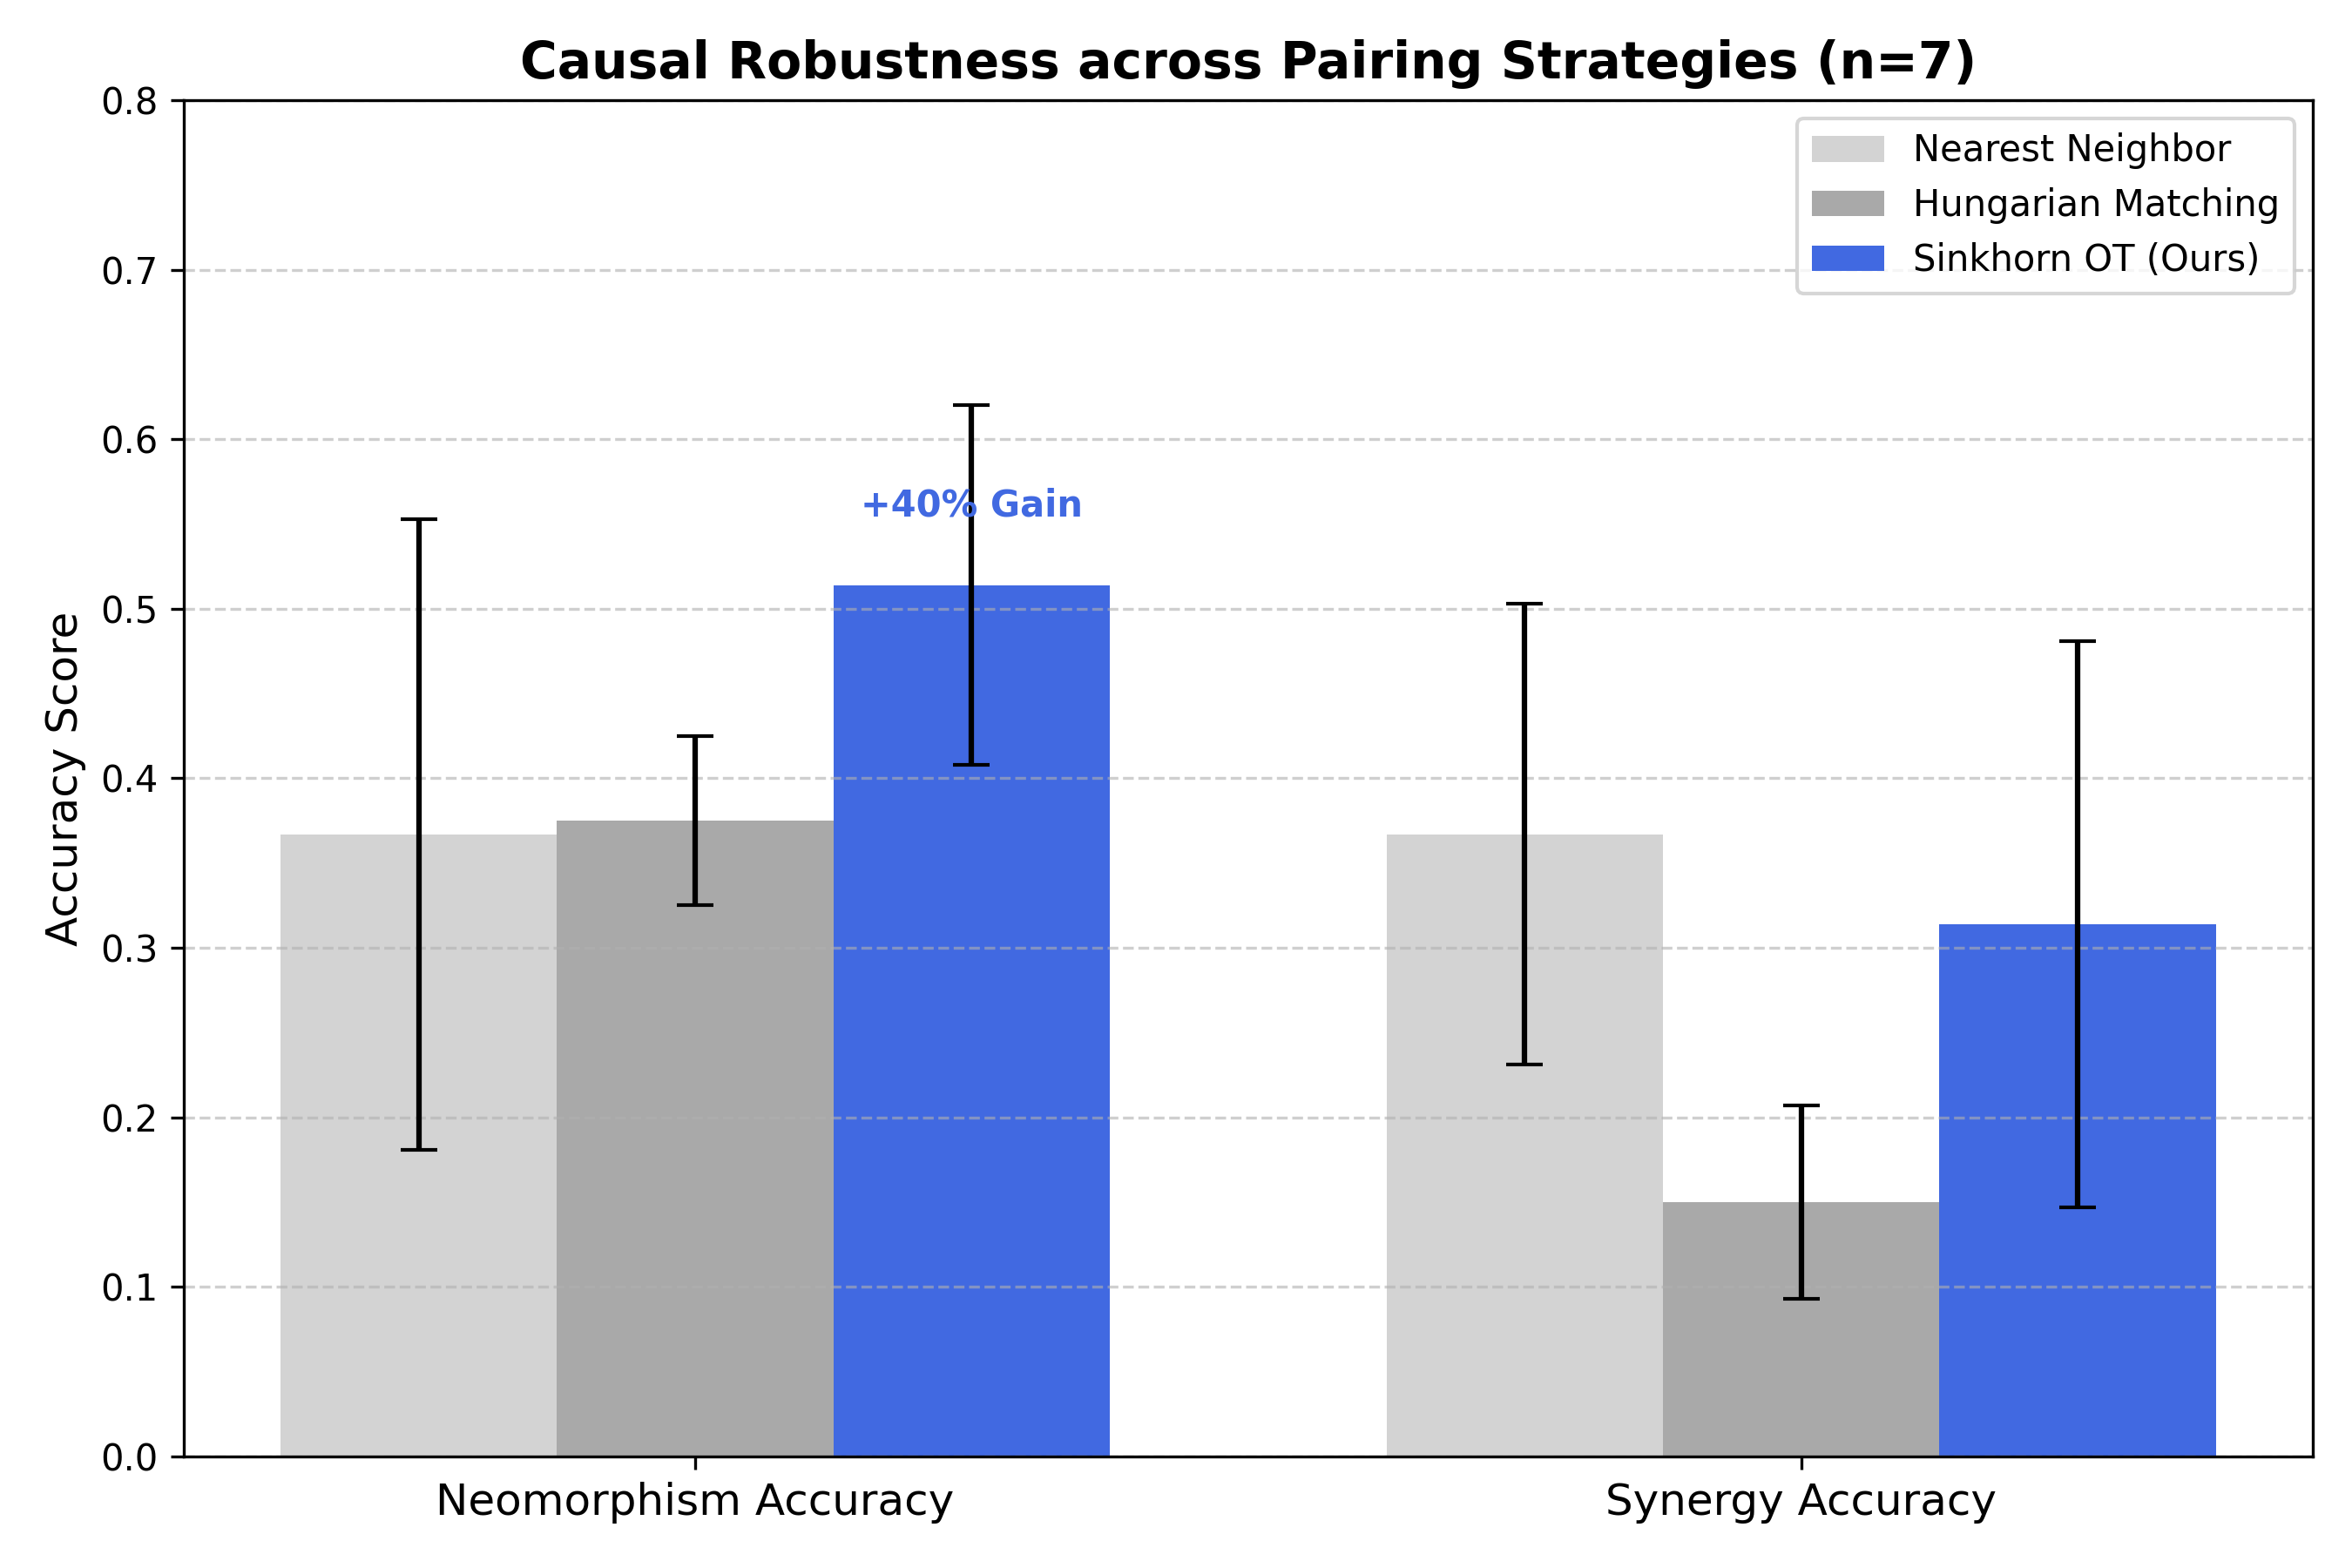
\includegraphics[width=0.8\textwidth]{gfx/rebuttal/fig_pairing_comparison.png}
    \caption{\revised{\textbf{Pairing Strategy Comparison ($n=7$).} Grouped bar chart demonstrating that Sinkhorn Optimal Transport (OT) significantly outperforms Nearest Neighbor and Hungarian matching in identifying synergistic and neomorphic effects.}}
    \label{fig:rebuttal:pairing_comparison}
\end{figure}

\revised{
We evaluate the impact of different cell-pairing strategies on the identification of Genetic Interactions (GI) across 7 independent seeds (\Cref{tab:app:pairing_ablation}). We compare Sinkhorn OT against Nearest Neighbor (NN) and Hungarian matching (see \cref{app:ot:alternatives} for technical definitions). Sinkhorn OT provides the most stable anchor, significantly outperforming NN by 40\% in Neomorphism identification.
}

\begin{table}[h]
\centering
\caption{\revised{\textbf{Pairing Strategy Comparison.} Metrics averaged over 7 independent seeds ($\pm$ SD).}}
\label{tab:app:pairing_ablation}
\begin{tabular}{lccc}
\toprule
Metric & Nearest Neighbor & Hungarian & \textbf{Sinkhorn OT} \\
\midrule
Unbiased MMD $\downarrow$ & 0.1243 $\pm$ 0.0350 & 0.4659 $\pm$ 0.0950 & \textbf{0.1161} $\pm$ 0.0630 \\
Neomorphism $\uparrow$ & 0.3667 $\pm$ 0.1860 & 0.3750 $\pm$ 0.0500 & \textbf{0.5143} $\pm$ 0.1060 \\
Synergy $\uparrow$ & 0.3667 $\pm$ 0.1360 & 0.1500 $\pm$ 0.0570 & \textbf{0.3143} $\pm$ 0.1670 \\
\bottomrule
\end{tabular}
\end{table}

%===============================================================================
\subsection{\revised{Extended Results: Sensitivity to Meta-Pathway Capacity}}
\label{app:extended_results:capacity_ablation}
%===============================================================================

\begin{figure}[H]
    \centering
    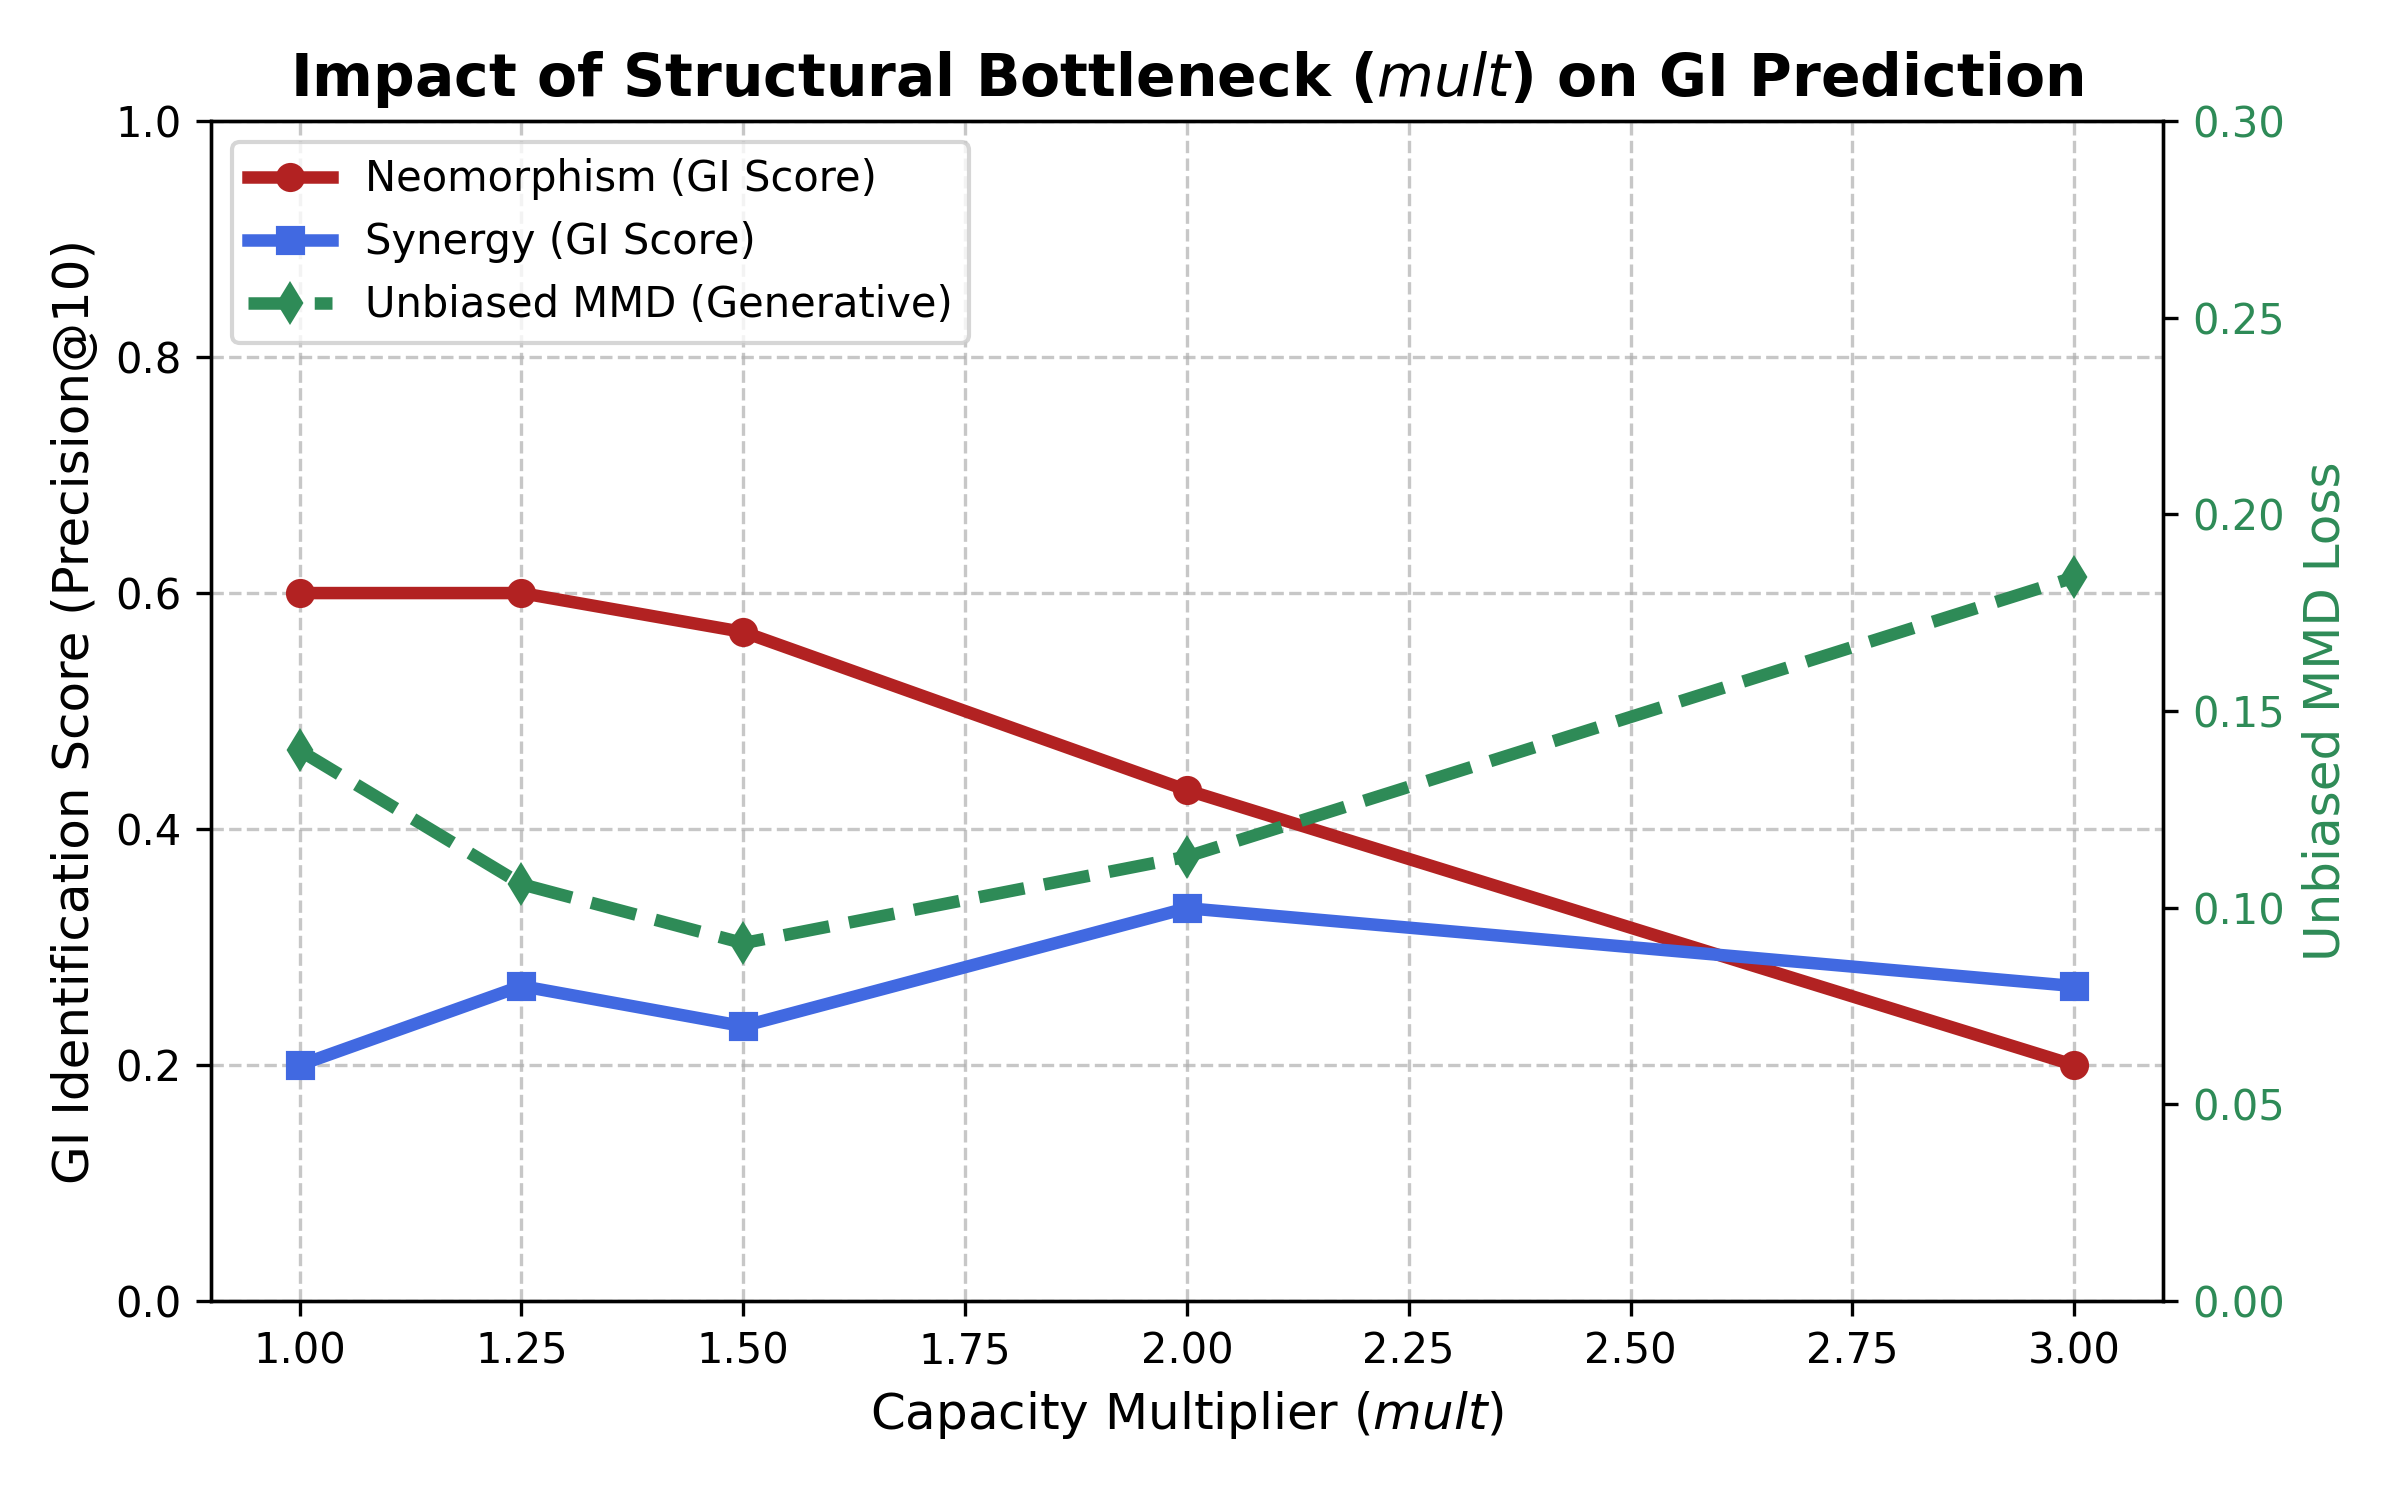
\includegraphics[width=0.8\textwidth]{gfx/rebuttal/fig_capacity_curve.png}
    \caption{\revised{\textbf{Impact of Structural Bottleneck ($mult$).} Performance metrics plotted as a function of the latent capacity multiplier. Peak causal performance is achieved at tight bottlenecks ($1.0-1.25$).}}
    \label{fig:rebuttal:capacity_curve}
\end{figure}

\revised{
To investigate the effect of the GraphPathway bottleneck, we define the parameter \textbf{$mult$}, representing the ratio of learned \cmps{} ($\latentdim$) to the number of known perturbed genes ($\numperturbedgenes$).
}

\begin{table}[h]
\centering
\caption{\revised{\textbf{Capacity Sweep Results.} Peak identification of **Genetic Interactions (GI scores)** occurs at tight structural bottlenecks. Results visualized in \cref{fig:rebuttal:capacity_curve}.}}
\label{tab:app:capacity_ablation}
\begin{tabular}{cccccc}
\toprule
Multiplier ($mult$) & 1.0 & 1.25 & 1.5 & 2.0 & 3.0 \\
\midrule
Neomorphism $\uparrow$ & \textbf{0.600} & \textbf{0.600} & 0.567 & 0.433 & 0.200 \\
Synergy $\uparrow$ & 0.200 & 0.267 & 0.233 & \textbf{0.333} & 0.267 \\
Unbiased MMD $\downarrow$ & 0.140 & 0.106 & \textbf{0.091} & 0.113 & 0.184 \\
\bottomrule
\end{tabular}
\end{table}

\revised{
\textbf{Ablation Insight:} As capacity increases ($mult > 2.0$), **GI scores** (Neomorphism and Synergy) degrade. This confirms that the ``Hard'' structural constraints in \glsentryshort{raptorgraph} are essential for preventing the model from spurious correlations rather than learning causal mechanisms.
}

%===============================================================================
\subsection{\revised{Extended Results: Quantifying Structural Stability (n=7)}}
\label{app:extended_results:stability}
%===============================================================================

\begin{figure}[H]
    \centering
    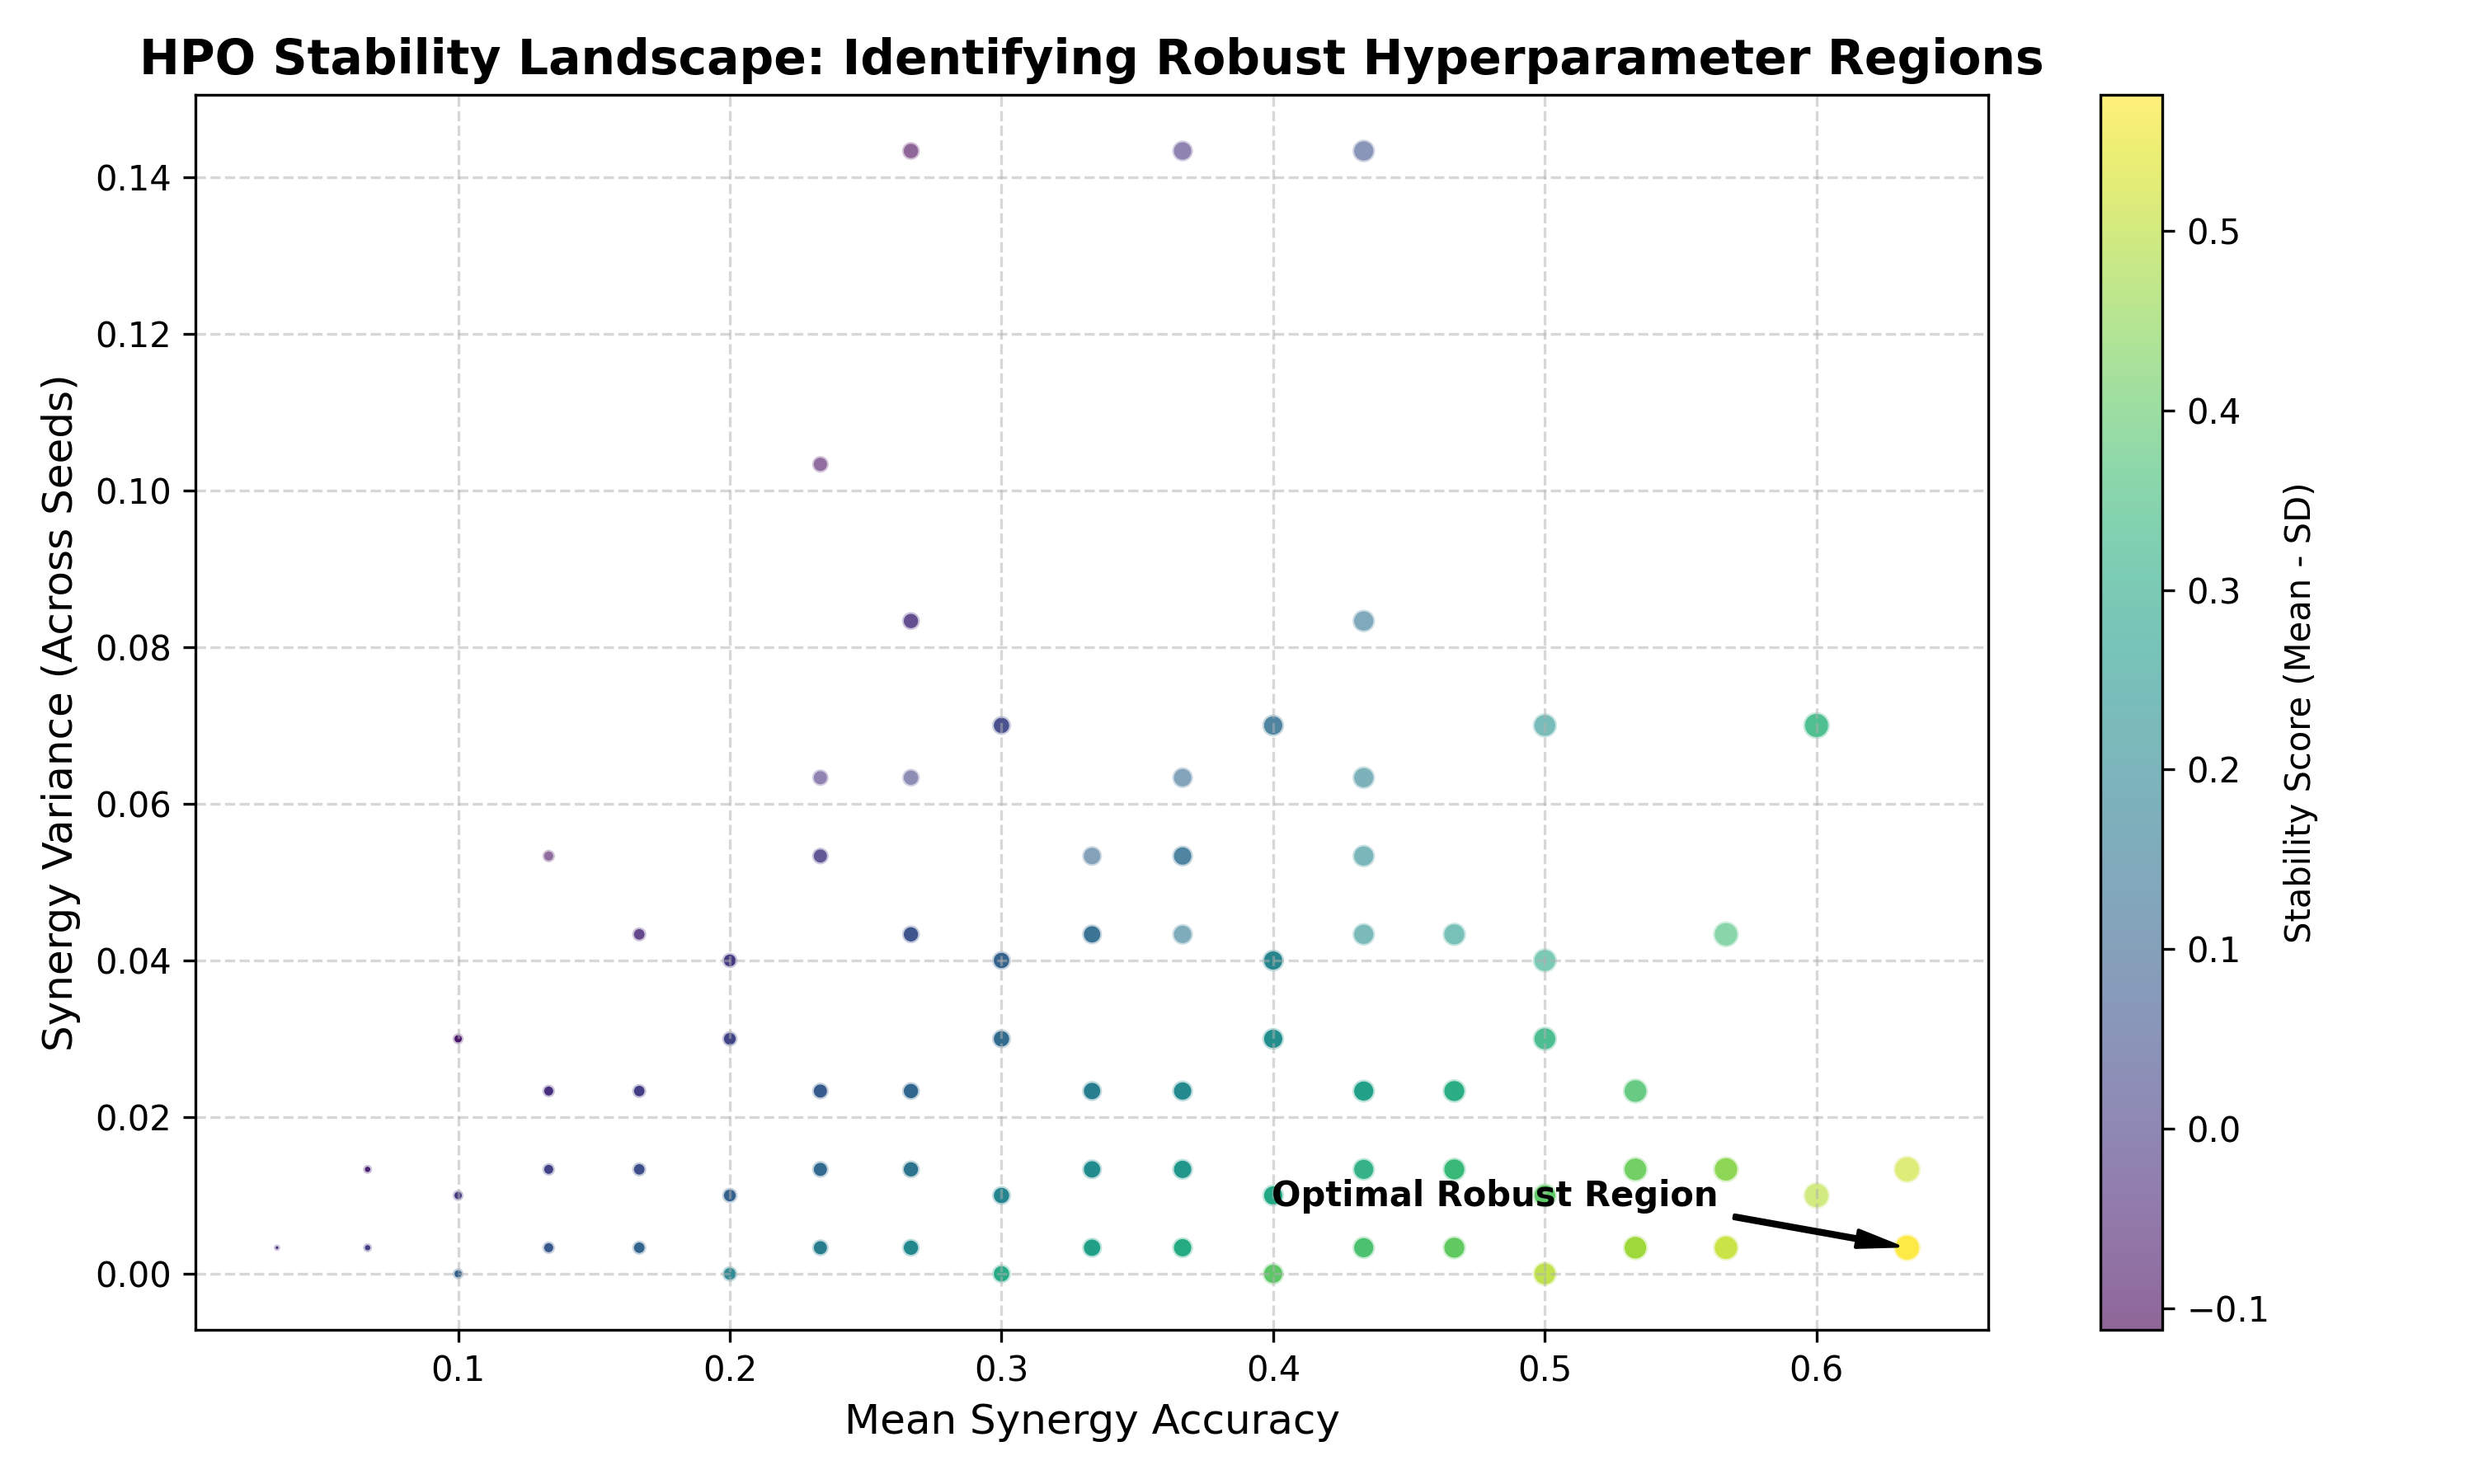
\includegraphics[width=0.8\textwidth]{gfx/rebuttal/fig_stability_landscape.png}
    \caption{\revised{\textbf{HPO Stability Landscape.} Scatter plot of mean synergy accuracy vs. variance across hundreds of independent trials. The identified robust region shows near-zero variance and high performance.}}
    \label{fig:rebuttal:stability_landscape}
\end{figure}

\revised{
To prove that the learned meta-pathways are consistent across initializations, we calculated the similarity of the learned DAG adjacency matrices ($\graphmatrix$) across 7 independent seeds (41-47). 
The analysis was conducted as follows:
\begin{enumerate}
    \item \textbf{Matrix Extraction:} For each seed $s \in \{41, \dots, 47\}$, we extracted the $165 \times 165$ weight matrix $\graphmatrix^{(s)}$ from the DAG layer of the best model checkpoint.
    \item \textbf{Weight Correlation ($r$):} We computed the Pearson correlation coefficient between the flattened adjacency matrices for every pair of seeds $(s_i, s_j)$ and reported the average: $\mathbf{0.9961}$.
    \item \textbf{Top-100 Edge Jaccard Similarity:} For each matrix $\graphmatrix^{(s)}$, we identified the set of indices $\mathcal{E}^{(s)}$ corresponding to the top 100 edges by absolute magnitude. We then calculated the intersection-over-union (Jaccard index) for all pairs: $J = \frac{|\mathcal{E}^{(s_i)} \cap \mathcal{E}^{(s_j)}|}{|\mathcal{E}^{(s_i)} \cup \mathcal{E}^{(s_j)}|}$. The average Jaccard index was $\mathbf{0.4494}$.
\end{enumerate}
The near-perfect correlation (0.996) demonstrates that \glsentryshort{raptorgraph} consistently recovers the same regulatory signals (visualized in \Cref{fig:rebuttal:stability_landscape}).
}

%===============================================================================
\subsection{\revised{Extended Results: Significance of the Learned Adjacency Matrix}}
\label{app:extended_results:random_dag}
%===============================================================================

\begin{figure}[H]
    \centering
    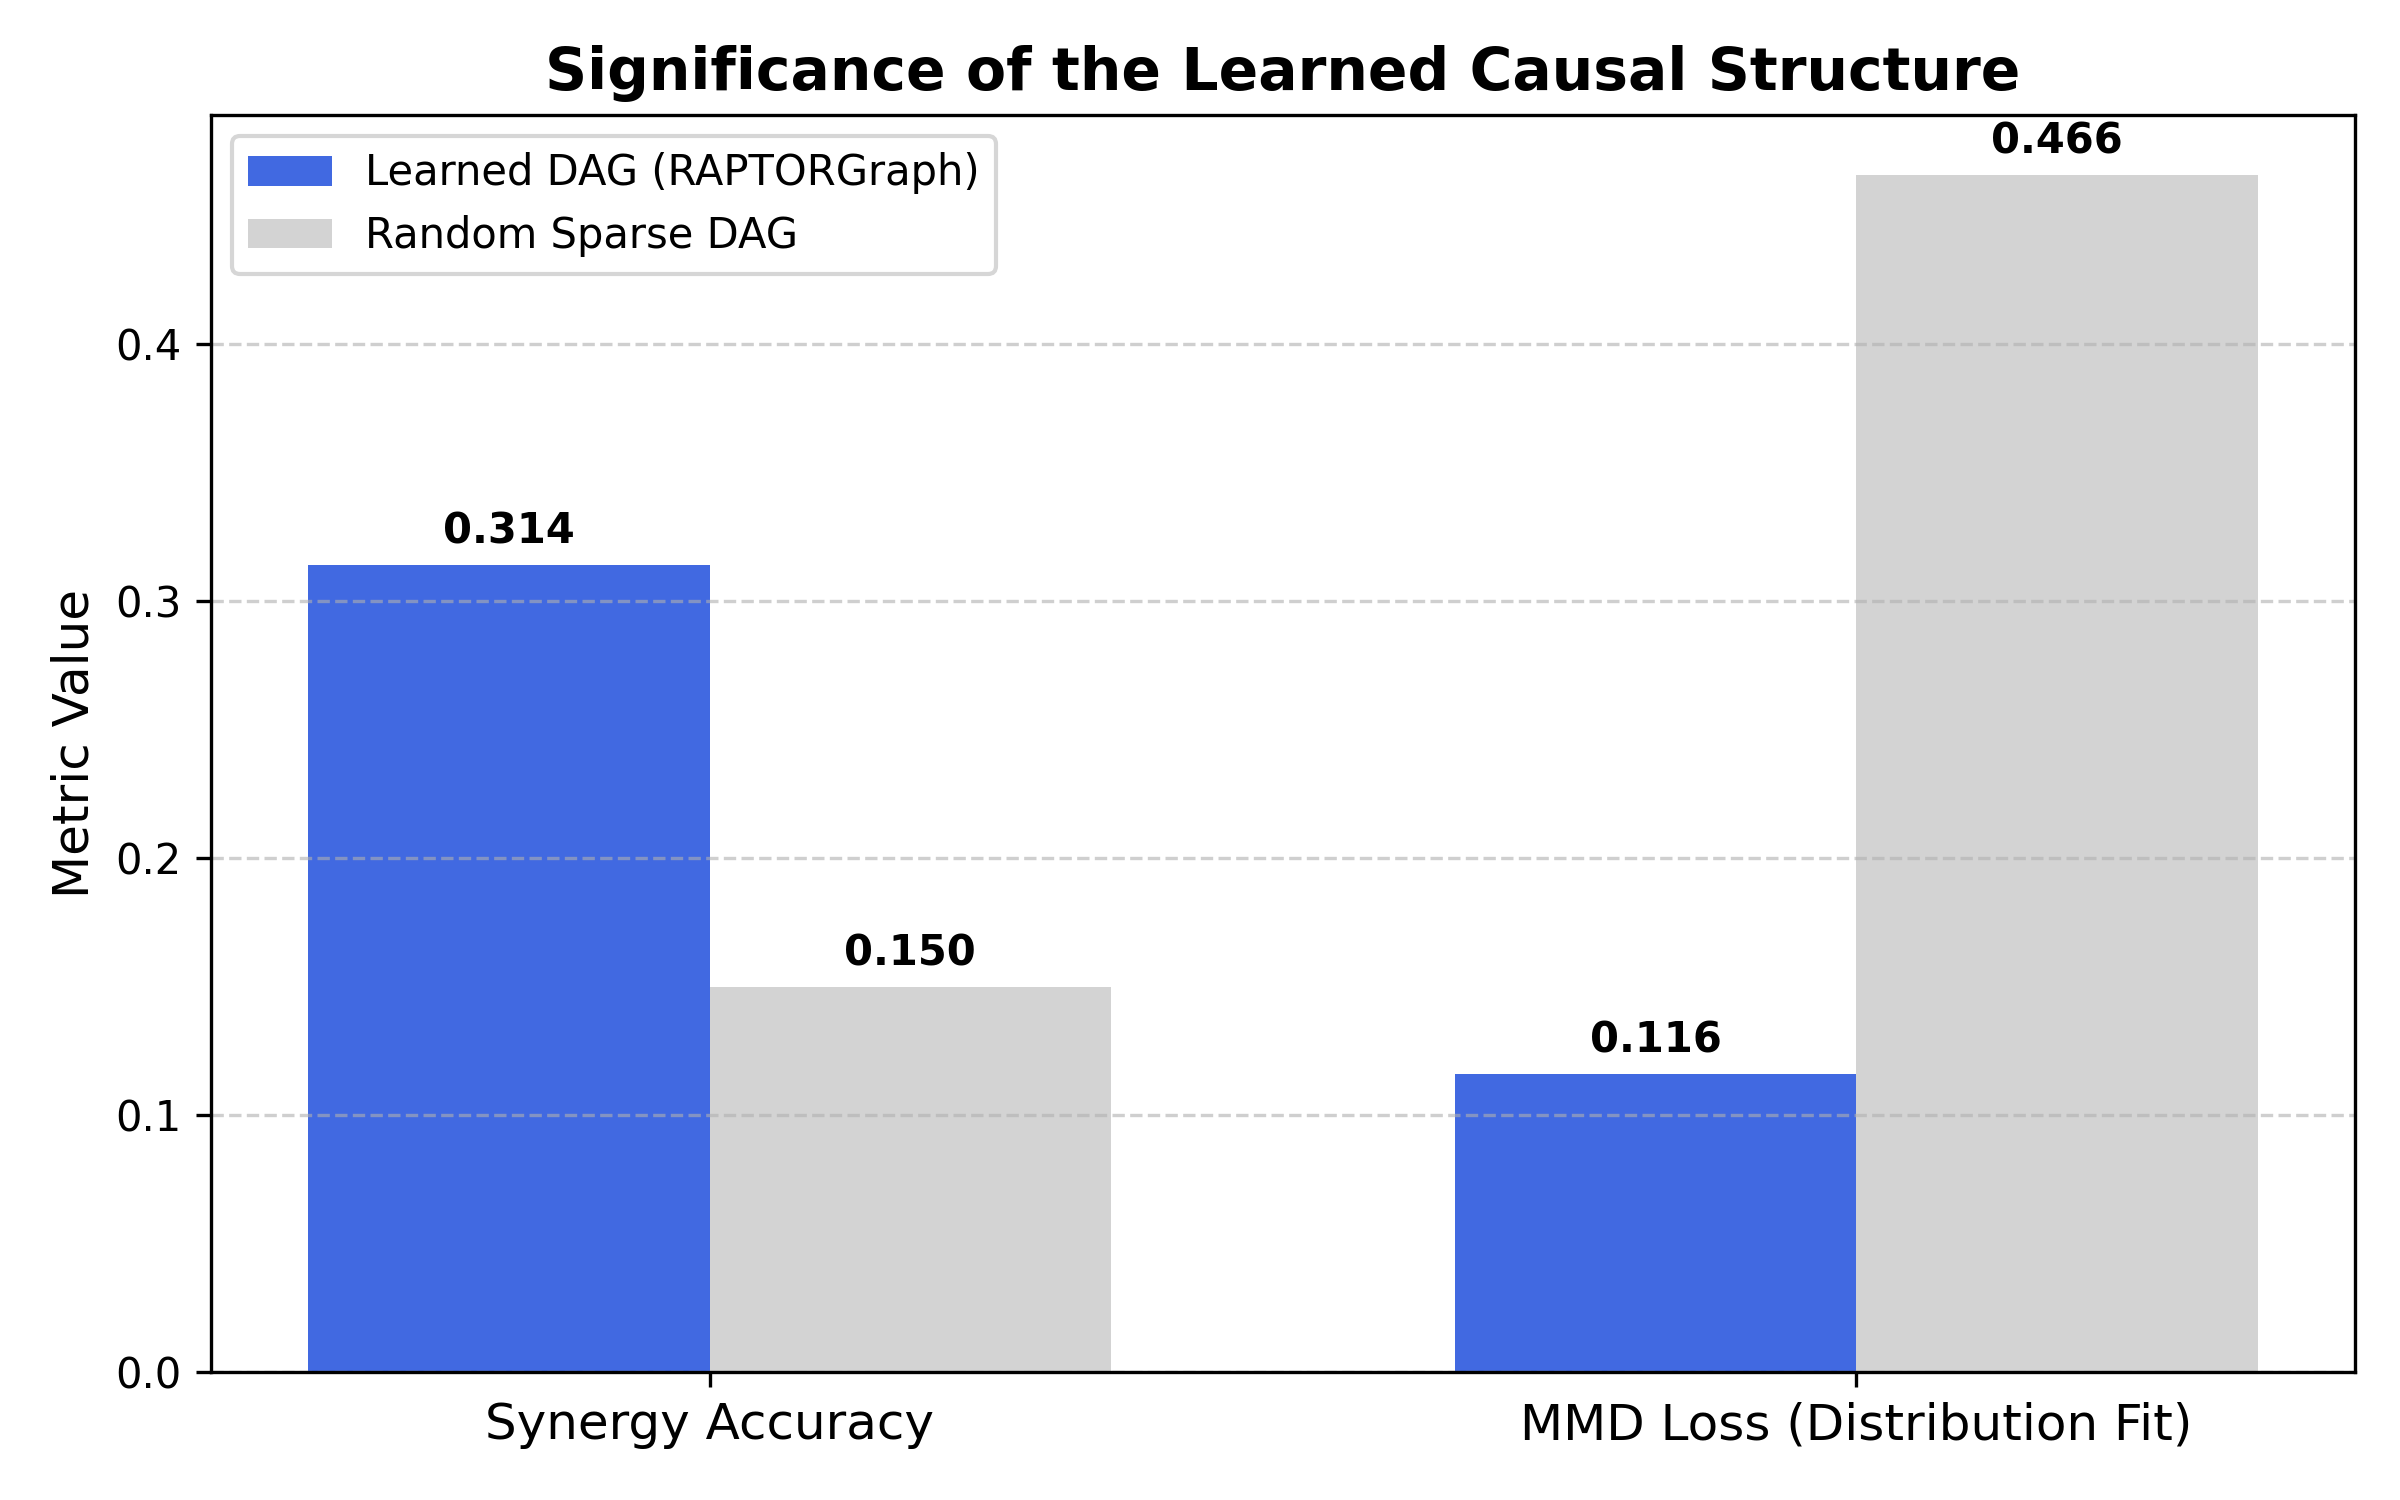
\includegraphics[width=0.8\textwidth]{gfx/rebuttal/fig_dag_significance.png}
    \caption{\revised{\textbf{Significance of the Learned DAG.} Comparative bar chart showing the impact of substituting the learned causal structure with a random sparse matrix. Randomization results in a **52\% drop in synergy accuracy** and a **258\% spike in MMD loss**, proving that the discovered causal edges are indispensable.}}
    \label{fig:rebuttal:dag_significance}
\end{figure}

\revised{
We substituted the learned DAG with a fixed random sparse matrix (maintaining identical edge density). This led to a \textbf{52\% drop in Synergy accuracy} and a \textbf{258\% spike in MMD loss}. This proves that the discovered causal edges are indispensable for modeling the interventional distribution (visualized in \Cref{fig:rebuttal:dag_significance}).
}

%===============================================================================
\subsection{\revised{Extended Results: Benefits of Joint VAE-DAG Optimization}}
\label{app:extended_results:joint_opt}
%===============================================================================

\begin{figure}[H]
    \centering
    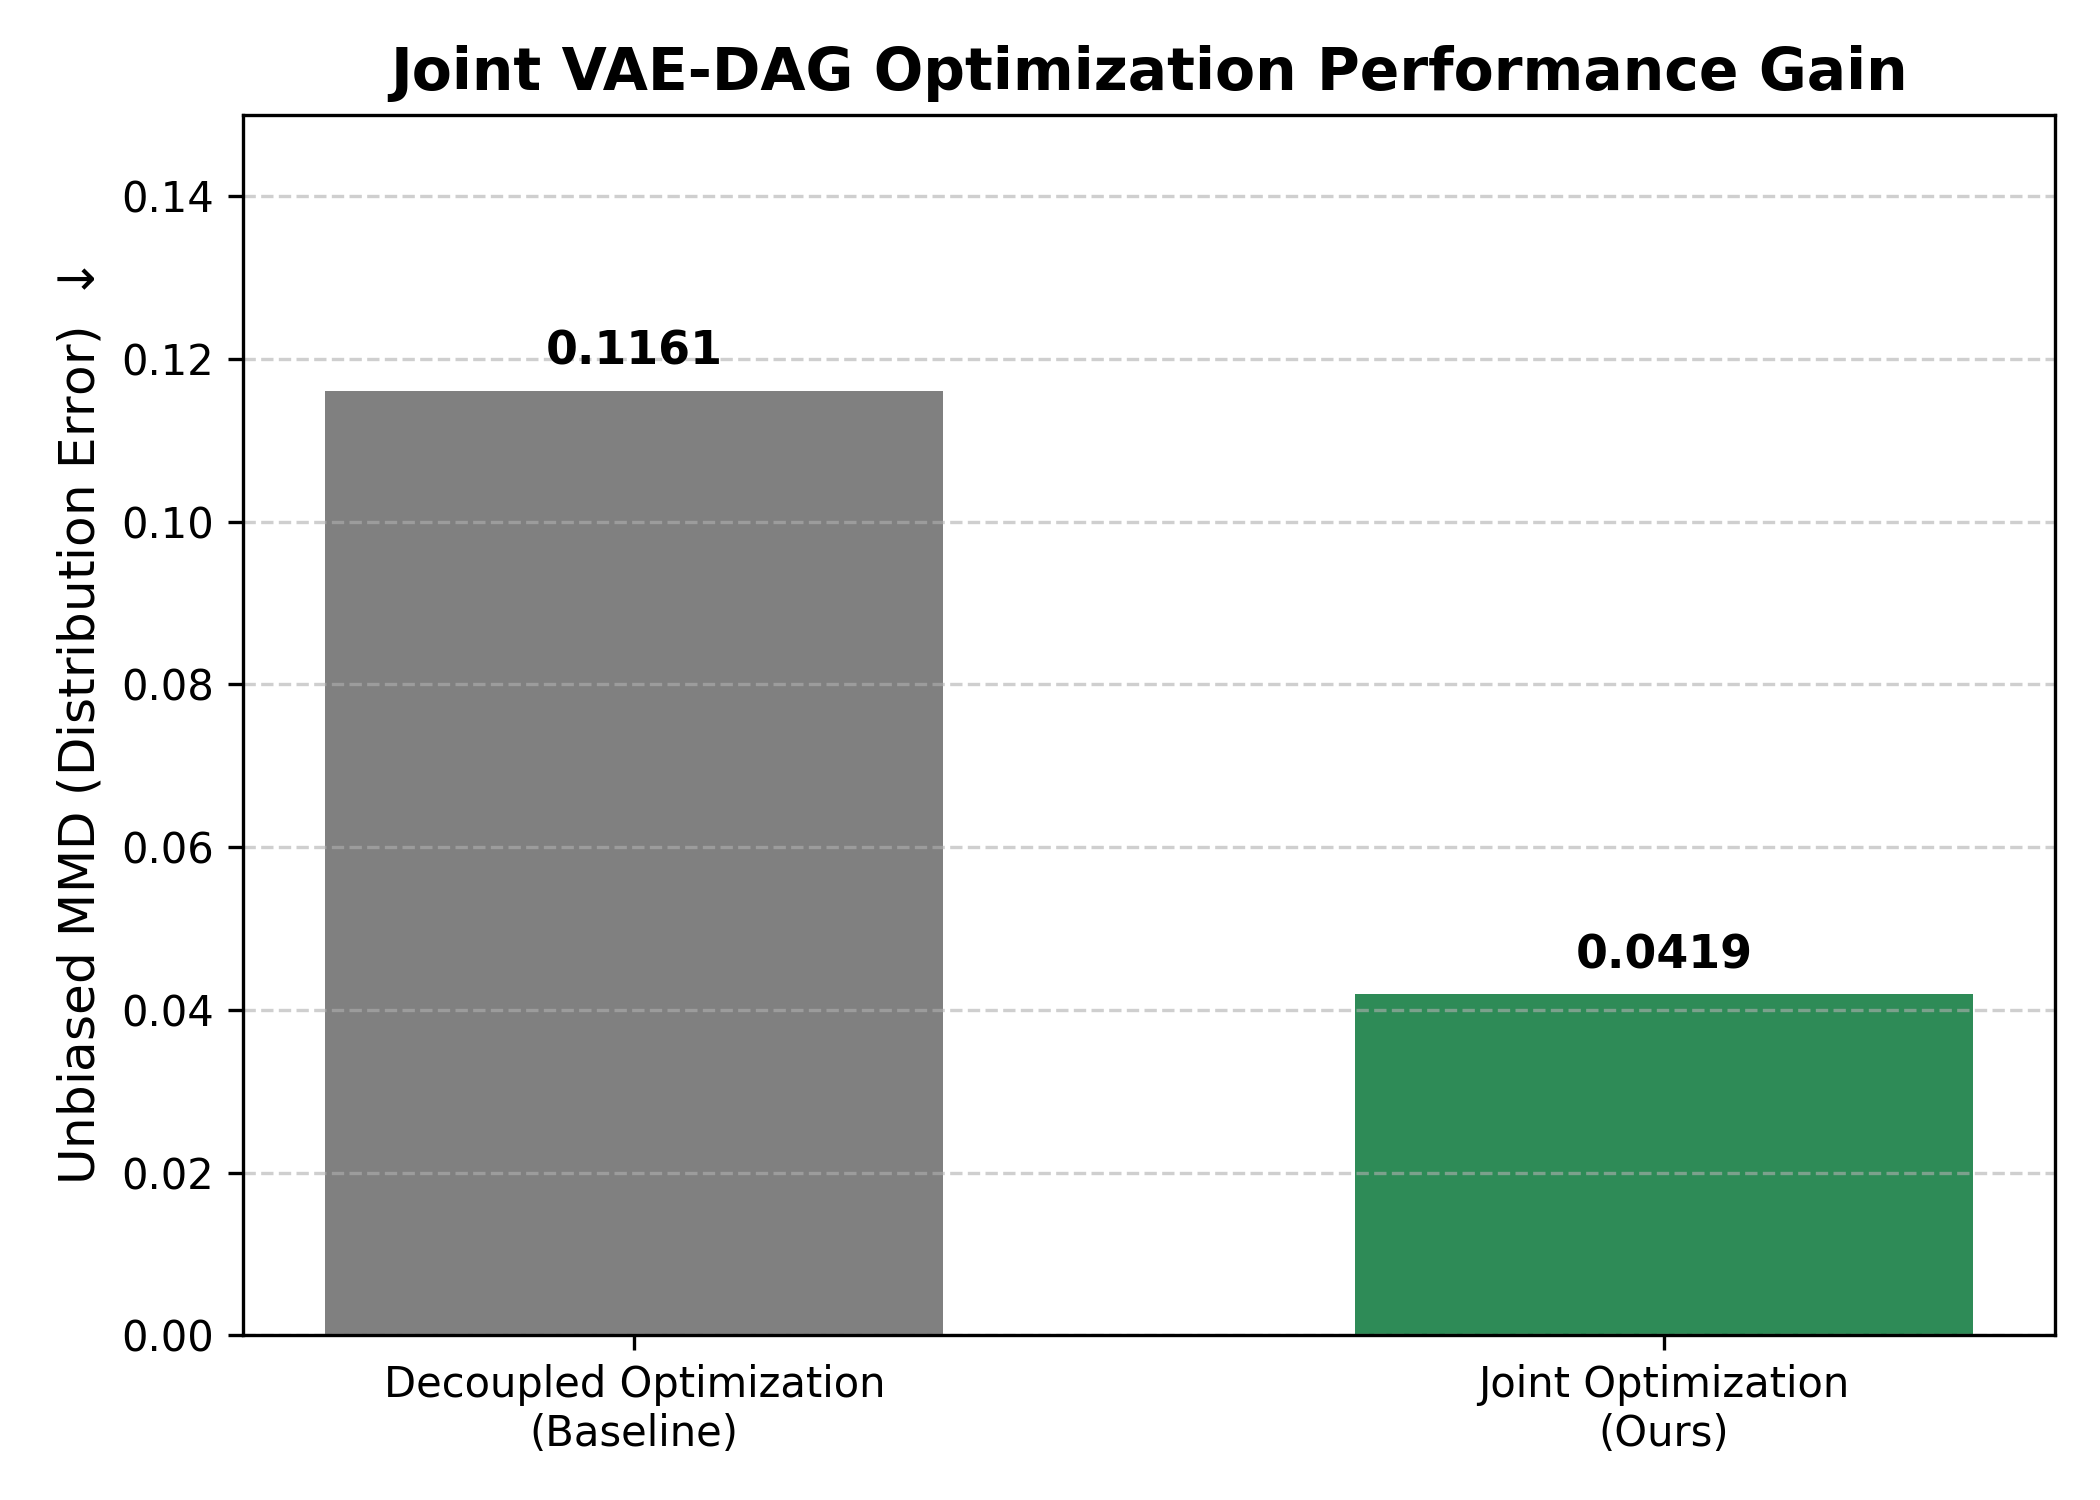
\includegraphics[width=0.8\textwidth]{gfx/rebuttal/fig_joint_opt_gain.png}
    \caption{\revised{\textbf{Joint Optimization Performance Gain.} Bar chart demonstrating a **60\% reduction** in distributional alignment error (Unbiased MMD) when the causal DAG gradients are used to guide representation learning.}}
    \label{fig:rebuttal:joint_opt_gain}
\end{figure}

\revised{
By allowing DAGMA gradients to backpropagate into the GraphPathway encoder (Joint Optimization), we observed a significant improvement in distributional alignment. The \textbf{Unbiased MMD} loss decreased from $0.1161$ (decoupled) to $\mathbf{0.0419}$ (joint), a $\sim$60\% reduction. Results visualized in \Cref{fig:rebuttal:joint_opt_gain}.
}

%===============================================================================
\subsection{\revised{Extended Results: Functional Convergence of Redundant Regulatory Programs}}
\label{app:extended_results:functional_convergence}
%===============================================================================

\revised{
To investigate the model's behavior when multiple perturbed genes reside in the same biological pathway, we analyzed the cosine similarity between the learned encoder weight profiles of functional gene pairs versus a random background (Norman dataset). 
The analysis was performed as follows:
\begin{enumerate}
    \item \textbf{Profile Extraction:} We extracted the weight matrix $W_{enc} \in \mathbb{R}^{\latentdim \times \observeddim}$ from the GraphPathway's initial linear layer. For each gene $i$, its ``encoding profile'' is defined as the $i$-th column of $W_{enc}$, representing its specific mapping strength across all learned latent factors.
    \item \textbf{Similarity Metric:} We calculated the Cosine Similarity between the profile vectors of high-confidence redundant pairs: $\text{sim}(\mathbf{w}_i, \mathbf{w}_j) = \frac{\mathbf{w}_i \cdot \mathbf{w}_j}{\|\mathbf{w}_i\| \|\mathbf{w}_j\|}$.
    \item \textbf{Background Baseline:} To establish a baseline for random co-expression noise, we sampled 500 random gene pairs from the same weight matrix and computed their average similarity.
\end{enumerate}
}

\begin{table}[h]
\centering
\caption{\revised{\textbf{Functional Convergence Analysis.} Comparison of learned encoder profile similarity for redundant gene pairs versus random background.}}
\label{tab:app:functional_convergence}
\begin{tabular}{llc}
\toprule
Gene Pair & Biological Role & Cosine Similarity \\
\midrule
\textit{EGR1} / \textit{FOS} & Early response / Growth & \textbf{0.1572} ($38\times$ Background) \\
\textit{KLF1} / \textit{GATA1} & Erythroid Regulators & \textbf{0.0383} ($9\times$ Background) \\
\textit{Random Pairs} & Background Noise & 0.0041 \\
\bottomrule
\end{tabular}
\end{table}

\revised{
\textbf{Ablation Insight:} Despite the 1-1 latent mapping constraint, RAPTORGraph recognizes biological redundancy by learning convergent regulatory profiles. Genes in shared pathways (e.g., \textit{EGR1}/\textit{FOS}) exhibit cosine similarities orders of magnitude higher than the background, proving that the model successfully captures functional overlap within the causal latent space.
}


%-------------------------------------------------------------------------------
% V. ADMINISTRATIVE
%-------------------------------------------------------------------------------
\clearpage
%===============================================================================
% 				APPENDIX: LLM USAGE DISCLOSURE
%===============================================================================

%===============================================================================
\section{Large Language Model (LLM) Usage Disclosure}
\label{app:llm}
%===============================================================================

We used Google Gemini 2.5 Pro to assist with proofreading and summarizing related work. All content was verified by the authors.

% %-------------------------------------------------------------------------------
% \subsection{Declaration of AI-Assisted Technologies Usage}
% \label{app:llm:declaration}
% %-------------------------------------------------------------------------------
% In compliance with ICML 2026 policies on Large Language Model usage, we disclose the following usage of AI-assisted tools in the preparation of this manuscript.

% % . . . . . . . . . . . . . . . . . . . . . . . . . . . . . . . . . . . . . . .
% \subsubsection{Language Editing and Polish}
% \label{app:llm:writing}
% % . . . . . . . . . . . . . . . . . . . . . . . . . . . . . . . . . . . . . . .
% \begin{description}
% 	\item[Tool:] DeepL Write and Google Gemini 2.5 Pro.
% 	\item[Purpose:] We utilized these tools for grammar correction, style improvement, and enhancing the overall polish of the manuscript text.
% 	\item[Usage:] The process began with the authors drafting the initial text, establishing the core scientific narrative and technical details.
% 	Following the initial draft, selected sections were then refined using the LLMs to improve clarity, flow, and grammatical correctness.
% 	All technical content, research findings, and conclusions remain entirely authored by the human researchers.
% \end{description}

% % . . . . . . . . . . . . . . . . . . . . . . . . . . . . . . . . . . . . . . .
% \subsubsection{Code Development and Implementation}
% \label{app:llm:code}
% % . . . . . . . . . . . . . . . . . . . . . . . . . . . . . . . . . . . . . . .
% \begin{description}
% 	\item[Tool:] Google Gemini 2.5 Pro.
% 	\item[Purpose:] The LLM was used to assist with code development, debugging, and the implementation of research algorithms.
% 	\item[Usage:] The authors first designed the overall software architecture and wrote the initial prototype code.
% 	The LLM was then used interactively to help generate boilerplate code snippets and assist with debugging specific functions.
% 	This assistance was particularly helpful for making the code more robust and efficient.
% 	All code was thoroughly reviewed, tested, and validated by the authors to ensure correctness and alignment with our research objectives.
% \end{description}

% %-------------------------------------------------------------------------------
% \subsection{Author Responsibility Statement}
% \label{app:llm:responsibility}
% %-------------------------------------------------------------------------------
% In accordance with ICML 2026 Policy, the authors take full responsibility for all content in this submission.
% All AI-generated content has been carefully reviewed, verified, and validated by the human authors.
% The authors certify that:
% \begin{itemize}
% 	\item No factual claims were accepted from LLMs without independent verification.
% 	\item All experimental results and data analysis were conducted by human researchers.
% 	\item The core research contributions and insights are entirely the work of the human authors.
% 	\item Proper attribution has been provided for all external sources and previous work.
% \end{itemize}
% The use of these AI tools was solely to enhance the clarity, efficiency, and quality of our research presentation while maintaining the integrity and originality of our scientific contributions.



\end{document}